\documentclass[%
	corpo=11pt,
    twoside,
    stile=classica,
    oldstyle,
    tipotesi=custom,
    greek,
    evenboxes,
]{toptesi}
%%%%%%%%%%%%%%%%%%%%%%%%%%%%%%%%%%%%%%%%%%%%%%%%%%%%

\usepackage{listings}
\usepackage{xcolor}

\definecolor{codegreen}{rgb}{0,0.45,0}
\definecolor{codegray}{rgb}{0.5,0.5,0.5}
\definecolor{codepurple}{rgb}{0.58,0,0.82}
\definecolor{backcolour}{rgb}{0.95,0.95,0.95.22}

\lstdefinestyle{mystyle}{
    backgroundcolor=\color{backcolour},   
    commentstyle=\color{codegreen},
    keywordstyle=\color{magenta},
    numberstyle=\tiny\color{codegray},
    stringstyle=\color{codepurple},
    basicstyle=\ttfamily\footnotesize,
    breakatwhitespace=false,         
    breaklines=true,                 
    captionpos=b,                    
    keepspaces=true,                 
    numbers=left,                    
    numbersep=5pt,                  
    showspaces=false,                
    showstringspaces=false,
    showtabs=false,                  
    tabsize=2
}

\lstset{style=mystyle}



\usepackage[utf8]{inputenc}
\usepackage[T1]{fontenc}
\usepackage{lmodern}

\usepackage{hyperref}
\hypersetup{%
    pdfpagemode={UseOutlines},
    bookmarksopen,
    pdfstartview={FitH},
    colorlinks,
    linkcolor={blue},
    citecolor={blue},
    urlcolor={blue}
  }

%%%%%%% use PDFLATEX 

\usepackage{stix}
\usepackage{epigraph}

\usepackage{lipsum} %to insert random text

\usepackage{geometry} %for the margins
\newcommand\fillin[1][4cm]{\makebox[#1]{\dotfill}} %for the dotted line in the frontispiace

\usepackage{dcolumn}
\newcolumntype{d}{D{.}{.}{-1} } %to vetical align numbers in tables, along the decimal dot

\usepackage{amsmath}

\usepackage{natbib} % for the bibliography
\bibliographystyle{plainnat}


%%%%%%% Local definitions
\newtheorem{osservazione}{Osservazione}% Standard LaTeX
\newtheorem{observation}{Observation}% Standard LaTeX




%%%%%%%%%%%%%%%%%%%%%%%%%%%%%%%%%%%%%%%%%%%%%%%%
%%%%%%%%%%%%%%%%%%%%%%%%%%%%%%%%%%%%%%%%%%%%%%%%



\begin{document}\errorcontextlines=9
%\english

\begin{titlepage}
\newgeometry{left=1cm,right=1cm,top=3cm,bottom=3.5cm}  %specific margins for this page

\begin{center}

{\huge POLITECNICO DI TORINO}\\[1.5cm]
\textbf{Corso di Laurea\\in Matematica per l'Ingegneria}\\[3cm]
%\textbf{Corso di Laurea Magistrale\\in Ingegneria Matematica}\\[3cm]

{\Large Tesi di Laurea}\\[1cm]
%{\Large Tesi di Laurea Magistrale}\\[0.5cm]
\textbf{\LARGE Filtraggio di immagini }\\[2cm]

\includegraphics[width=0.2\textwidth]{./Pictures/logo_polito_2021.jpg}
\vspace{4cm}


\begin{minipage}{0.85\textwidth}
\begin{flushleft}\large
\textbf{Relatori} \hfill \textbf{Candidato}\\
prof. Nome Cognome \hfill Raffaello Ippolito\\
prof. Nome Cognome \\
\textit{firma dei relatori} \hfill \textit{firma del candidato}\\[0.35cm]
\fillin\ \hfill \\
\fillin\ \hfill \fillin
\end{flushleft}
\end{minipage}

\vfill

Anno Accademico 2021-2022
\end{center}

\restoregeometry %restor default margins 

\end{titlepage} %the frontispiece

%%%%%%% Dedication
\ifclassica%
\begin{dedica}

    $\heartsuit$\ All'autrice di "Passi" %Alla mia regina
\end{dedica}
%%%%%%% 

\sommario%summary
%Here goes the abstrat of your thesis

Le immagini sono da sempre state fondamentali per l'uomo, che sin dai primi tempi le ha utilizzate per ricordare, illustrare, comunicare, etc. Per questo motivo, cercare di sfruttarle nel migliore dei modi è oggigiorno un problema di grande interesse. Molteplici sono i metodi di elaborazione digitali detti "di filtraggio", il cui scopo è modificare l'immagine, estraendone elementi, nascondendoli o facendoli risaltare, così da migliorarla per renderla quanto più utile possibile agli scopi richiesti.\\
Durante questa trattazione, dopo una breve introduzione volta a fornire una visione d'insieme del campo in esame (nel quale ci si sta introducendo), verrà illustrato il concetto di immagine digitale, di filtro e di equazioni alle derivate parziali, con particolare riguardo al ruolo fondamentale che queste ultime giocano nella scrittura dei filtri e la relativa implementazione all'interno del calcolatore.\\
Nello specifico, nella parte introduttiva si parlerà della storia delle immagini digitali e del filtraggio analogico e digitale, dei principali problemi consequenziali e di alcune delle più semplici elaborazioni digitali. Verranno poi fornite alcune nozioni preliminari tra cui: il concetto di immagine come funzione matematica e quindi di immagine digitale, della relativa codifica, di pixel, del concetto di risoluzione ed altresì di quanto essa influisca sullo spazio di archiviazione. Successivamente saranno analizzati i filtri intesi come convoluzioni tra la funzione immagine e la funzione filtro.\\
Infine la trattazione diventerà più specifica, presentando il fulcro di questo studio, ossia l'implementazione del metodo Perona-Malik; a sostegno di ciò verrà illustrato il metodo delle differenze finite per l'approssimazione delle derivate parziali con relativa analisi dell'errore di troncamento. Questo risultato sarà dunque sfruttato per la realizzazione di uno script MATLAB che operi l'equazione del calore e che verrà poi opportunamente modificato per implementare il metodo Perona-Malik.   

%Lo studio delle Equazioni alle derivate parziali ed il loro impiego in ambito di filtraggio di immagini.

%%%%%%%%%%%%%%%%%%%%%%%%%%%%%%%%%%%%%%%%%%%%%%%%
%%%%%%%%%%%%%%%%%%%%%%%%%%%%%%%%%%%%%%%%%%%%%%%%

\ringraziamenti%acknowledgements
%Acknowledge the people you love and/or work with
I candidati ringraziano vivamente il Granduca di Toscana per i mezzi messi loro a disposizione, ed il signor Von Braun, assistente del prof.~Albert Einstein, per le informazioni riservate che egli ha gentilmente fornito loro, e per le utili discussioni che hanno permesso ai candidati di evitare di riscoprire l'acqua calda.

Questa parte è rimasta inalterata da com'era nel template.

%%%%%%%%%%%%%%%%%%%%%%%%%%%%%%%%%%%%%%%%%%%%%%%%
%%%%%%%%%%%%%%%%%%%%%%%%%%%%%%%%%%%%%%%%%%%%%%%%

%\tablespagetrue
\figurespagetrue%to include the list of tables
%and the list of figures - yuo can comment these commands

\indici%table of content
%It automatically generated

%%%%%%%%%%%%%%%%%%%%%%%%%%%%%%%%%%%%%%%%%%%%%%%%
%%%%%%%%%%%%%%%%%%%%%%%%%%%%%%%%%%%%%%%%%%%%%%%%

%Citation
%If you feel like a poetic guy!
\ifclassica   
\begin{citazioni}
    \textit{If you cannot understand my\\argument, and declare}\\
    it's Greek to me\\
    \textit{you are quoting Shakespeare.}
    
    [\textsc{B. Levin}, Quoting Shakespeare]\vspace{1em}
\end{citazioni}
\fi

%%%%%%%%%%%%%%%%%%%%%%%%%%%%%%%%%%%%%%%%%%%%%%%%
%%%%%%%%%%%%%%%%%%%%%%%%%%%%%%%%%%%%%%%%%%%%%%%%

\mainmatter

\newpage
\chapter{Introduzione}
\chapter{Storia del filtraggio e principali problemi affrontati}

L'essere umano, da sempre, sfrutta i propri sensi per relazionarsi con il mondo.  \\Il suo primo riferimento in particolare è la vista, senza la quale egli si sente perso, smarrito; per questo è fondamentale sviluppare un linguaggio  visivo che sia efficace. \\ La società contemporanea sfrutta immagini di vario genere (fotografie, radiografie, ecografie, poster pubblicitari, progetti, etc.) per comunicare messaggi e/o per rendere chiari progetti, idee, situazioni.\\
\`E quindi un problema sempre di grande interesse cercare di sfruttarle al meglio. A tal proposito esistono alcuni metodi di "filtraggio", la cui finalità è quella di migliorare la qualità delle immagini, metterne in risalto determinate caratteristiche o nasconderne delle altre.


%Da sempre l'essere umano si affida continuamente alla propria vista; la percezione visiva, infatti, è il primo mezzo di interfaccia con la realtà circostante senza il quale l'individuo si sente perso, smarrito.\\
%Per questo motivo è fondamentale per l'uomo comunicare attraverso un linguaggio visivo, la società contemporanea, conscia di ciò, sfrutta immagini di vario genere e nei campi più disparati 




%Le immagini hanno un ruolo fondamentale nelle nostre vite, viviamo di immagini, ne guardiamo tutti i giorni in tutti i contesti, la percezione visiva è sempre il nostro primo riferimento senza la quale ci si sentiamo persi.\\
%Viviamo in una società consapevole di ciò e che sfrutta questo aspetto quanto più possibile nei campi più disparati, fotografie, radiografie, ecografie, poster pubblicitari, progetti, etc.\\
%E' quindi un problema sempre di grande interesse cercare di sfruttarle al meglio, a tal fine esistono metodi cosìdetti di "filtraggio", tramite i quali intendiamo migliorare la qualità delle nostre immagini, mettere in risalto determinate caratteristiche o nasconderne altre.


\section{Filtraggio analogico}
Anche prima dell'avvento dei computer esisteva l'elaborazione delle immagini. Esistevano infatti dei procedimenti, detti “mascherature”, che servivano a ridurre o esaltare le differenze di luce nella foto.\\
La mascheratura avveniva durante la fase di stampa su carta, ossia quando il negativo veniva proiettato sulla carta fotografica mediante l’ingranditore.



\vspace{1em}\noindent 
Qui, %lo “stampatore” 
l'operatore usava una serie di metodi per far si che su certe zone della carta andasse più o meno luce di quella che sarebbe arrivata passando attraverso il negativo.

Ad esempio la tecnica nota come "altissimo contrasto" permetteva di avere foto con soli bianchi e soli neri, il viraggio invece serviva a dare un tono di colore alla foto, che restava comunque un bianco e nero: famoso il viraggio tono seppia.

%\vspace{1em} \noindent
\section{Immagini digitali}
Le prime applicazioni delle immagini digitali sono state sui giornali negli anni 20. Non esistevano veri e propri computer, il segnale era trasmesso tramite telegrafo simulando dei mezzitoni.
In particolare, il sistema di trasmissione di immagini via cavo Bartlane era una tecnica inventata nel 1920 per trasmettere immagini di giornali digitalizzate su linee sottomarine tra Londra e New York.




\noindent Il sistema di trasmissione di immagini via cavo Bartlane generava sia sul trasmettitore che sul ricevitore una scheda dati perforata o un nastro che veniva ricreato come immagine.

\begin{figure}[htb] \centering
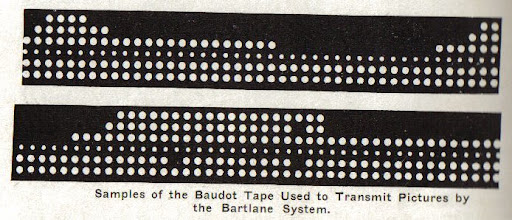
\includegraphics[scale=0.7, trim = 0 1.1cm 0 0, clip]{Pictures/nastro Bartlane.jpg}
\caption{Nastro dati codificante un'immagine.}\label{fig:figura}
\end{figure}

\noindent
In questo modo riusciva a codificare immagini in bianco e nero in cinque diverse gradazioni di grigio, capacità poi ampliata a 15 gradazioni nel 1929.

\begin{figure}[htb] \centering
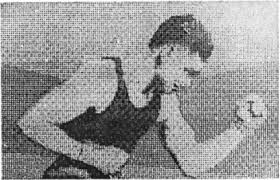
\includegraphics[scale=0.5, trim = 0 1.1cm 0 0, clip]{Pictures/img del 1921 a 5 gradazioni di grigio.jpg}
\qquad\qquad
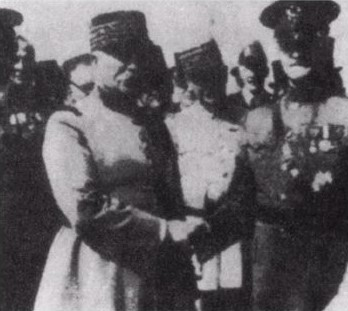
\includegraphics[scale=1.7, trim = 0 1.1cm 0 0, clip]{Pictures/img del 1929 a 15 gradazioni di grigio.jpg}
\caption{La prima immagine risale al 1921 ed è composta da 5 gradazioni di grigio.\\ 
La seconda è del 1929 ed è composta da 15 gradazioni di grigio.}\label{fig:figura}
\end{figure}
\vspace{1em} \noindent
Questa, in qualche modo, è la nascita delle immagini digitali, anche se non sono trattate da computer e quindi codificate in maniera differente. Inoltre in questa fase non abbiamo una vera e propria elaborazione delle immagini, ma solo una trasmissione e la successiva stampa.

\vspace{1em} \noindent
Nel 1957, Russell A. Kirsch produsse un dispositivo che generava dati digitali che potevano essere archiviati in un computer; questo utilizzava uno scanner a tamburo e un tubo fotomoltiplicatore.\\
Negli anni immediatamente successivi questo portò a notevoli sviluppi.

%\vspace{1em} \noindent
\section{Filtraggio digitale}
Nel 1960 presso il Jet Propulsion Laboratory, il Massachusetts Institute of Technology, i Bell Laboratories, l'Università del Maryland, e altre strutture di ricerca svilupparono molte delle tecniche di elaborazione digitale di immagini (o della trasformazione di immagini digitali come spesso veniva chiamata) al fine di evitare le debolezze operative delle fotocamere a pellicola per missioni scientifiche e militari.\\
Queste trovarono poi applicazione in immagini satellitari, immagini medicali, videocitofono, riconoscimento ottico dei caratteri, e miglioramenti fotografici.

Il costo dell'elaborazione in quel periodo era piuttosto alto con l'apparecchiatura di elaborazione. Le cose cambiarono negli anni settanta, quando computer più economici e hardware dedicato furono resi disponibili sul mercato.\\
Le immagini allora potevano essere elaborate in tempo reale, l'elaborazione digitale sostituisce così i vecchi metodi a pellicola per molti scopi.

\vspace{1em} \noindent
Negli anni 2000, grazie all'avvento di computer più veloci, l'elaborazione delle immagini digitali diventò la forma più comune di elaborazione delle immagini e, in generale, divenne il metodo più utilizzato data la sua versatilità e il basso costo.

La tecnologia di elaborazione delle immagini digitali per applicazioni mediche è stata inserita nel 1994 nella Hall of Fame della Space Foundation.



\newpage
\section{Nozioni introduttive}
La società moderna è una società digitale. Le immagini passano generalmente per un calcolatore prima di essere stampate, o in ogni caso possono essere sempre scannerizzate (con strumenti più o meno precisi) così da averne una copia digitale.
\`E in questa fase che l'immagine subisce il processo di filtraggio, nel calcolatore, quando è in formato digitale, Per capire cos'è un filtro occorre dunque chiedersi cosa sia un'immagine digitale.

\subsection{Immagini digitali}
\`E necessario comprendere a fondo cosa sia un oggetto, per poterlo poi implementare in un calcolatore, a tal scopo è utile quindi capire esattamente che cos'è un'immagine

\begin{quote}
\epigraph{\textit{Forma esteriore degli oggetti corporei, in quanto viene percepita attraverso il senso della vista, o si riflette – come realmente è, o variamente alterata – in uno specchio, nell’acqua e sim., o rimane impressa in una lastra o pellicola o carta fotografica.}}{Vocabolario Treccani}
\end{quote}

\noindent
Un'immagine viene rappresentata, impressa quindi su superfici, cioè oggetti bidimensionali, di dimensioni finite e le vediamo perchè i nostri occhi percepiscono il susseguirsi di colori diversi. Come codificare tali entità?
Come per tutti gli oggetti reali, sebbene abbiano dimensioni finite, le immagini sono distruibuzioni continue, o per meglio dire, il susseguirsi delle gradazioni di colore avviene in una maniera che possiamo considerare come continua. Questo è il primo problema che ci si pone quando si pensa a come codificare delle immagini.\\
La soluzione più largamente utilizzata è anche quella più semplice ed intuitiva, ossia di discretizzare tale distribuzione di colori. Si divide l'immagine con una griglia e ad ogni casella, che d'ora in poi chiameremo \textbf{pixel}, assegnamo un colore.
\`E ovvio che così facendo si perdono dei dettagli, la quantità di dettagli che riusciamo a conservare può variare enormemente, una minima quantità di dettagli si perde sempre ma è un prezzo che vale la pena pagare.
\newpage
Facciamo un esempio:

%\ref{fig:figuraa}. 
\begin{figure}[htb] \centering
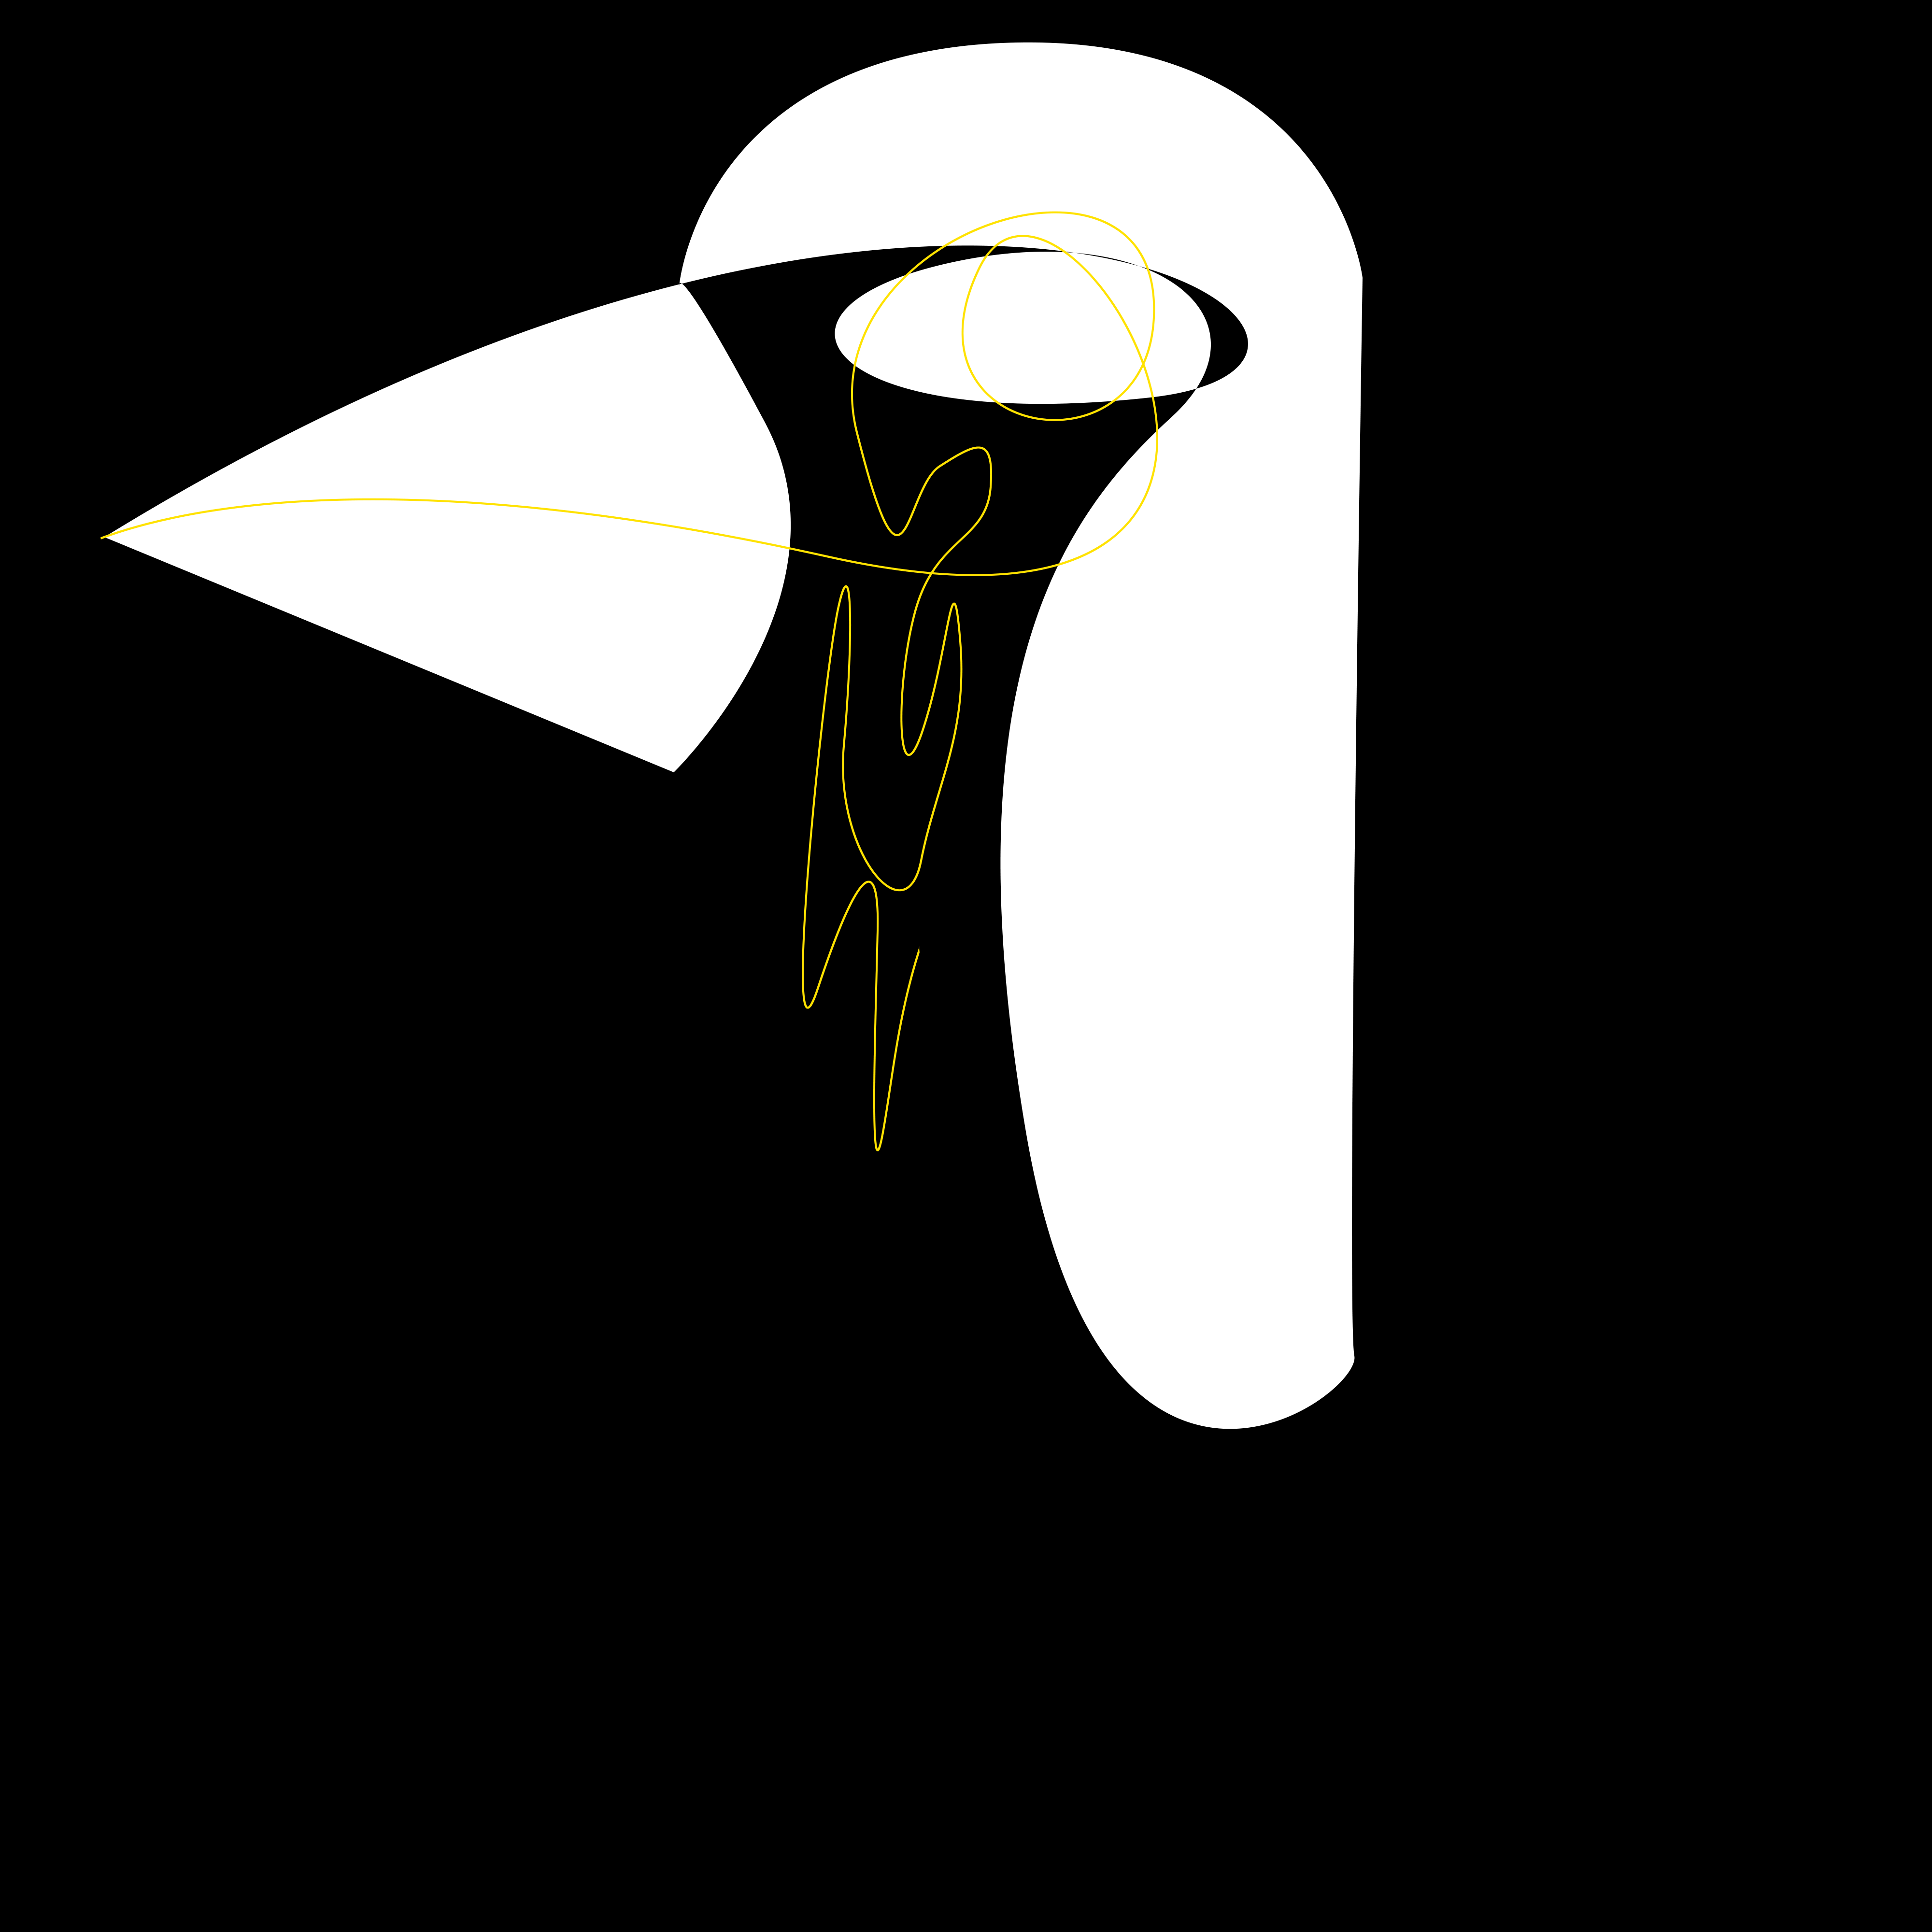
\includegraphics[scale=0.08]{Pictures/in ricordo del pinguino cameriere.png}
%\caption{Fiamme.}\label{fig:figura}
\qquad\qquad

\includegraphics[scale=0.08]{Pictures/canvas8x8.png}
\caption{Confronto tra immagine originale e immagine codificata utilizzando una griglia 4x4.}\label{fig:figura}
\end{figure}

%\ref{fig:figura}. 
\begin{figure}[htb] \centering
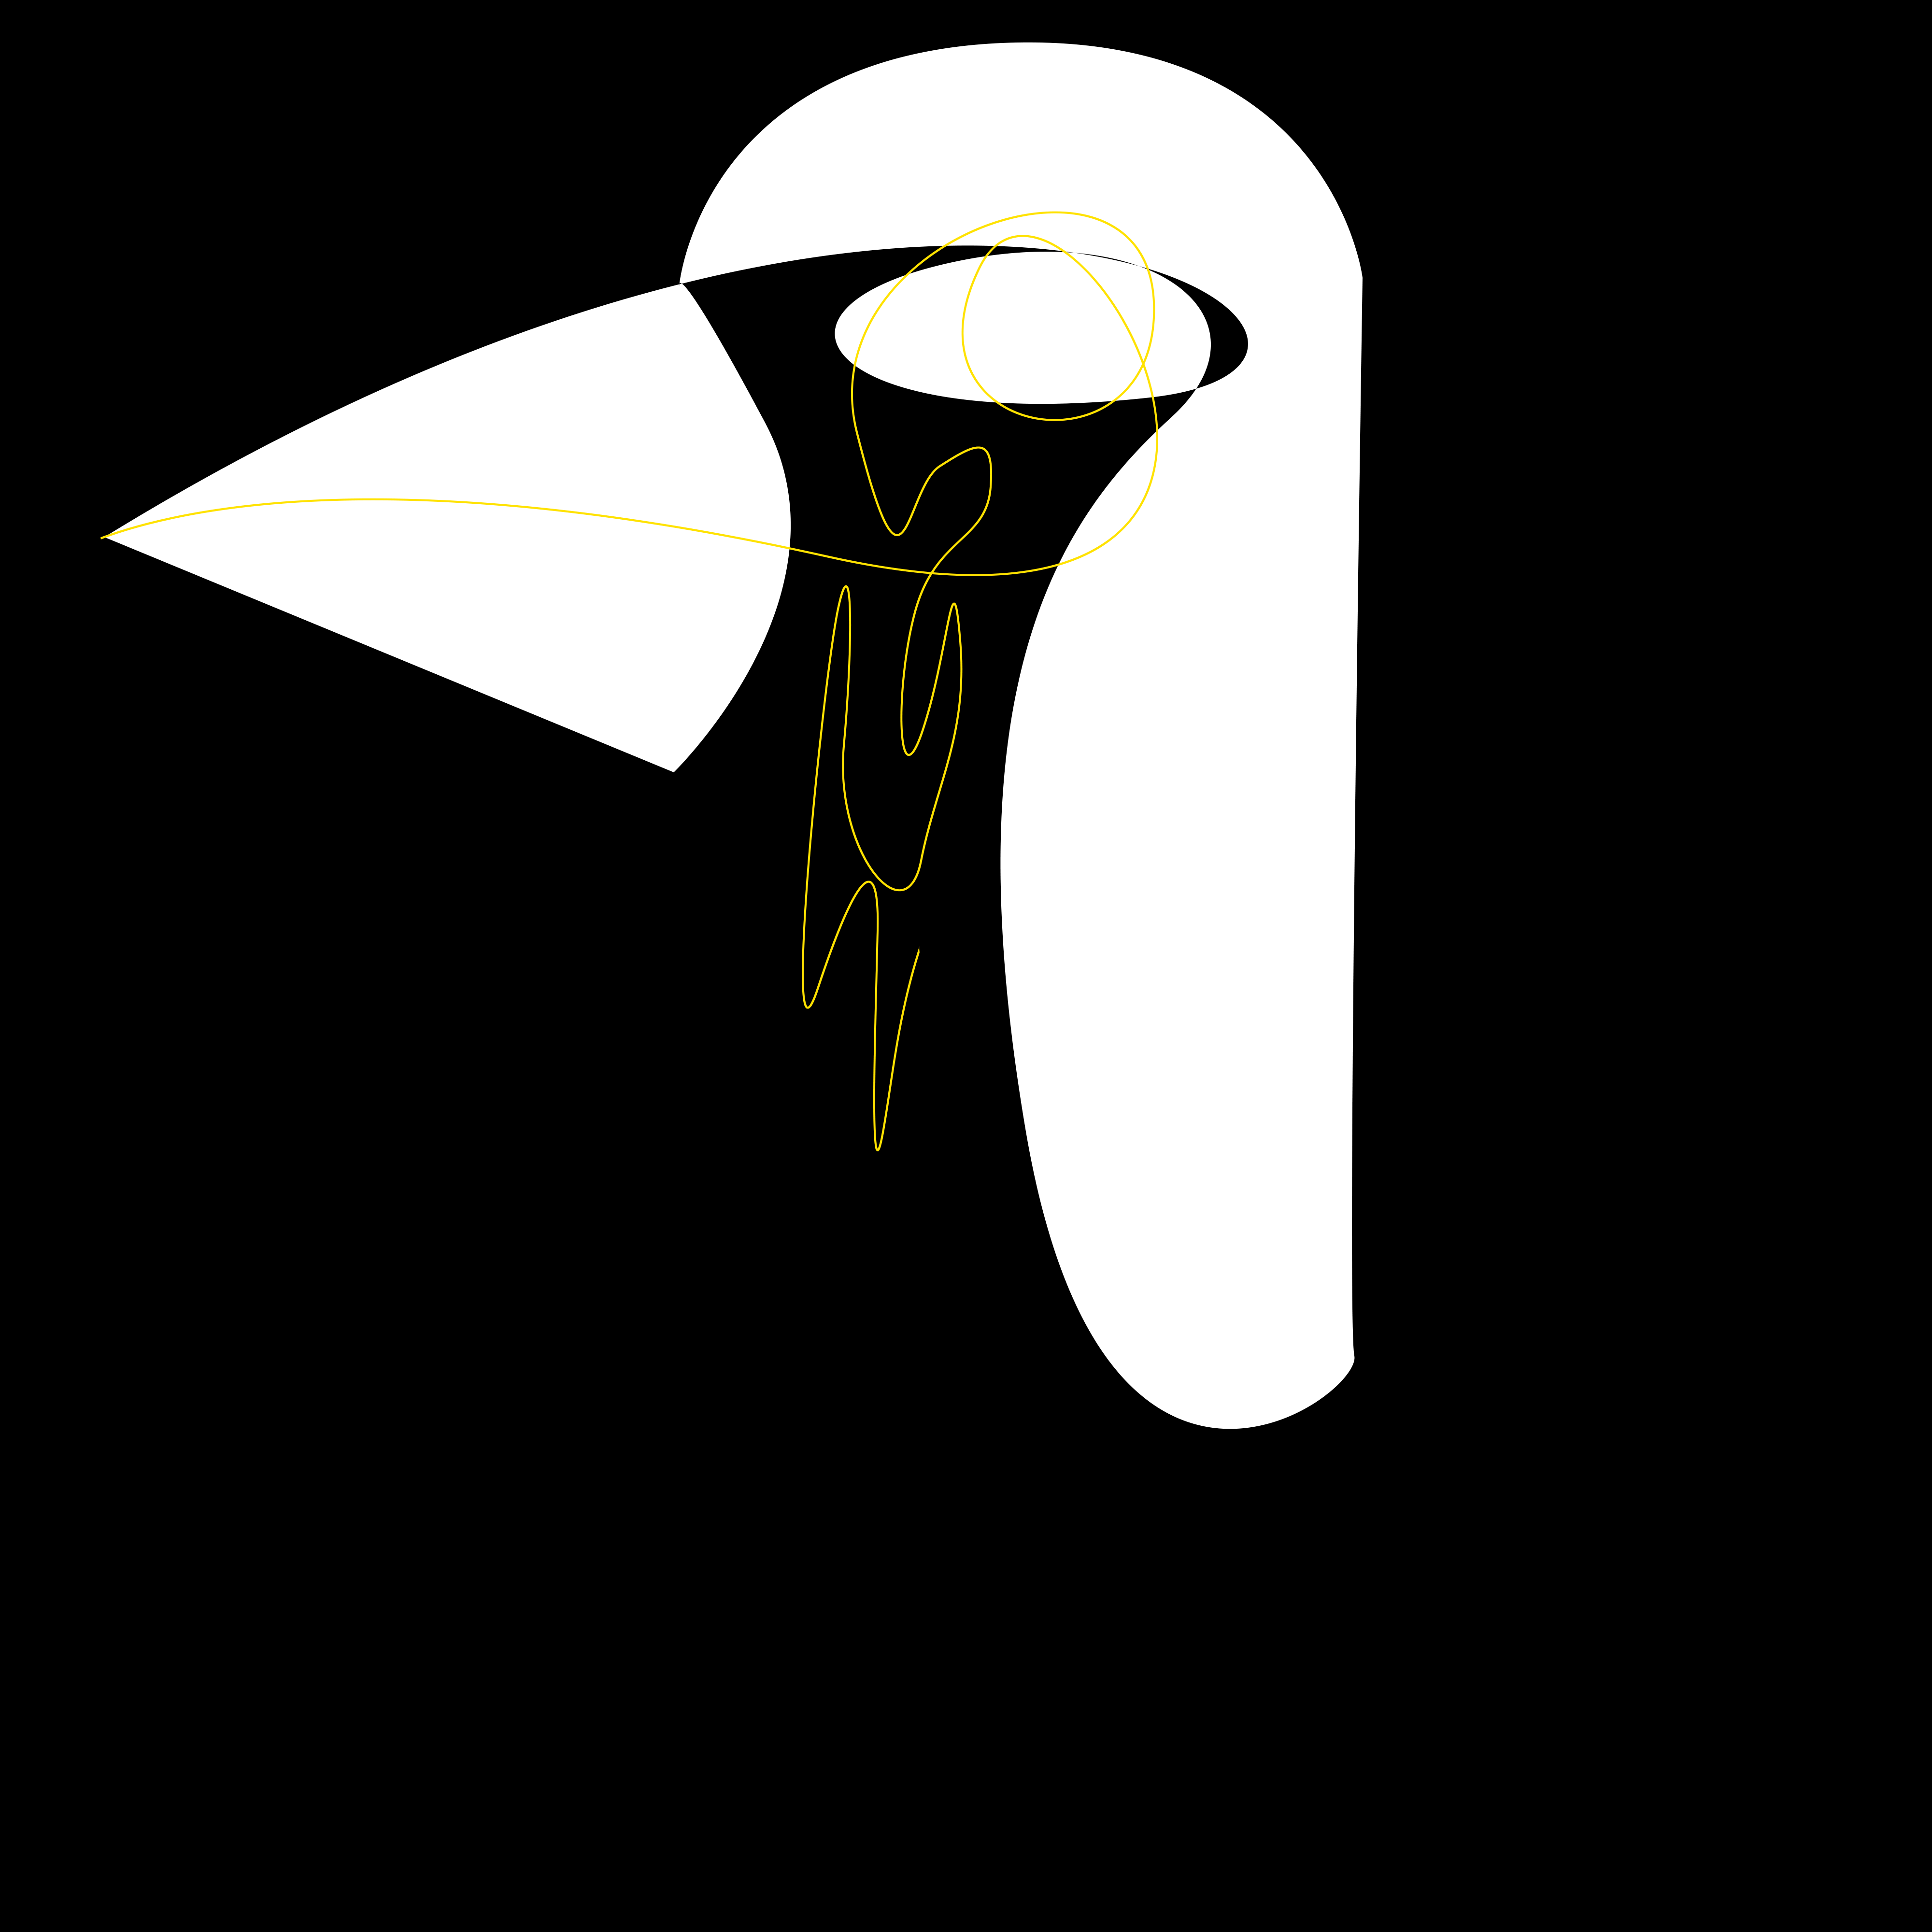
\includegraphics[scale=0.08]{Pictures/in ricordo del pinguino cameriere.png}
\qquad\qquad

\includegraphics[scale=0.08]{Pictures/canvas80x80.png}
\caption{Confronto tra immagine originale e immagine codificata utilizzando una griglia 80x80.}\label{fig:figura}
\end{figure}

\noindent
\`E semplice vedere come ad una griglia più fitta corrisponda una miglior qualità dell'immagine, questo è il concetto di \textbf{risoluzione di un'immagine}. 
Una miglior risoluzione però costa, come anticipato, in termini di memoria. Una griglia 4x4 corrisponde a 16 pixel, ad una griglia 80x80 corrispondono invece 6400 pixel! Questo vuol dire che la seconda immagine pesa 400 volte di più della prima.

\vspace{1em} \noindent
Volendo definire in maniera più precisa che cosa è un'immagine digitale, diremmo che quest'ultima è una funzione da $\mathbb R^2$ in $\mathbb R^3$ cioè, date in input due coordinate, essa restituisce un colore (che è formato da 3 canali RGB). Se però l'immagine è in bianco e nero la questione si semplifica: l'immagine diventa una funzione da $\mathbb R^2$ in $\mathbb R$, dal momento che per codificare un colore appartenente alla scala di grigio basta un solo canale: il livello di luminosità. Difatti, la riduzione da tre ad un solo canale rappresenta un grosso vantaggio, permettendo di diminuire di due terzi lo spazio di memoria occupato.

\subsection{Cosa sono i filtri}
Una volta capito che un'immagine è una funzione possiamo definire un filtro come una seconda funzione che convoluta alla prima da il risultato richiesto.\\
Una equazione alle derivate parziali (PDE) esprime una evoluzione. Sia u la nostra immagine e $u_0$ lo stato in cui si trova inzialmente, allora per convoluzione possiamo dire che 

\begin{equation} \label{eq:eq3}
u(x)=\frac{1}{w(x)}\int\int d(x-\xi)\Tilde{d}(u_0(x) -u_0(\xi))u_0(\xi)d\xi.
\end{equation}

\centering con  $w(x) = \int\int d(x-\xi)\Tilde{d}(u_0(x) -u_0(\xi))d\xi$ \cite{korn}\newline

\raggedright

In matematica, la \textbf{convoluzione} è un'operazione tra due funzioni di una variabile che consiste nell'integrare il prodotto tra la prima e la seconda traslata di un certo valore.

E questo è a tutti gli effetti un filtro. Il problema adesso è far eseguire questi calcoli ad un calcolatore, il quale non è in grado di lavorare con oggetti continui e richiede quindi di alcune approssimazioni per discretizzare il problema.

A tal proposito la definizione di convoluzione può facilmente essere discretizzata parlando di successioni anzichè di funzioni ed operando una sommatoria invece di un integrale.

$$
(f*g)[n]\ {\stackrel {{\mathrm {def}}}{=}}\ \sum _{{m=-\infty }}^{\infty }f[m]\,g[n-m]=\sum _{{m=-\infty }}^{\infty }f[n-m]\,g[m].
$$

Altri metodi ed approssimazioni saranno poi approfonditi durante la trattazione del problema

%Definiti questi concetti siamo pronti ad iniziare la trattazione vera e propria


%\newpage
\section{Principali problemi di elaborazione digitale}

Al giorno d'oggi i computer permettono una vasta gamma di elaborazioni digitali, ce ne sono alcuni, più semplici ma di notevole interesse, ormai già perfezionati ed altri che sono ancora oggetto di studio.

\subsection{Rotazioni, riflessioni,etc}
\cite{storia}
Le trasformazioni più semplici in assoluto riguardano movimenti rigidi come la \textbf{traslazione} o la \textbf{rotazione}, o anche omeomorfismi come la \textbf{riflessione}. Questi sono molto utili per introdurre i primi concetti matematici, come l'impiego di matrici.\\
Definiamo una \textbf{matrice di trasformazione} che moltiplicata per un vettore di coordinate ci restituisca un altro vettore di coordinate. Questo vuol dire che quel punto va spostato dalle coordinate in cui si trovava a quelle appena calcolate. Ad esempio:\\

$$
{\begin{bmatrix}
-1&0&0\\
0&1&0\\
0&0&1
\end{bmatrix}}
$$


\`E una matrice di riflessione lungo l'asse verticale, infatti: 

$$
{\begin{bmatrix}
-1&0&0\\
0&1&0\\
0&0&1
\end{bmatrix}}
\begin{bmatrix}
x\\y\\1
\end{bmatrix}
=
\begin{bmatrix}
-x&y&1
\end{bmatrix}
$$	

\vspace{1em} \noindent
Cioè ogni punto rimane alla stessa quota ma cambia la propria x con -x, che è esattamente ciò che si intende per riflessione lungo l'asse verticale.

\noindent 
Altri esempi possono essere:

\begin{align*}
&\begin{bmatrix}
1&0&0\\
0&-1&0\\
0&0&1
\end{bmatrix}&~&
\text{Riflessione lungo l'asse orizzontale}\\
\\
&\begin{bmatrix}
2&0&0\\
0&1.5&0\\
0&0&1
\end{bmatrix}&~&
\text{Scalamento}\\
\\
&\begin{bmatrix}
\cos(\theta )&\sin(\theta )&0\\
-\sin(\theta )&\cos(\theta )&0\\
0&0&1
\end{bmatrix}&~&
\text{Rotazione di un angolo theta}\\
\end{align*}



\subsection{Cambio prospettiva}
Una delle trasformazioni più semplici è quella del cambio prospettiva. Una volta compresa questa trasformazione si è fatto anche un primo passo per parlare di warping, che sarà trattato più avanti.

\vspace{1em} \noindent
Un esempio pratico può essere: si ha la foto di un documento poggiato su una scrivania e la si vuole migliorare in modo da estrarne solo il documento e che i suoi bordi concidano quindi con i bordi dell'immagine.

\vspace{1em} \noindent
In genere la cosa più semplice ed affidabile è quella di far scegliere i 4 angoli del documento ad un utente. Volendo automatizzare il processo si può però scegliere un'altra strada, ossia estrarre i bordi dell'immagine e cercare tra questi quelli che formano un trapezio; presumibilmente quello sarà il documento.

\vspace{1em} \noindent
Ottenuti i 4 angoli, occorre calcolare la lunghezza e la larghezza della nuova immagine. Per fare ciò si può calcolare la lunghezza dei 4 lati banalmente con il teorema di Pitagora. A questo punto, presi i lati a due a due non adiacenti, cioè che non hanno vertici in comune, ne si confrontano le lunghezze.\\
Per ogni coppia si adotta la lunghezza maggiore (si può anche usare quella minore ma è una scelta di scarso interesse per lo studio in atto).

\vspace{30em} \noindent
Ottenuti questi dati si può calcolare la matrice di trasformazione. Essa sarà del tipo:

\begin{align*}
&\begin{bmatrix}
a_1&a_2&b_1\\
a_3&a_4&b_2\\
c_1&c_2&1
\end{bmatrix}
\text{ dove }
\begin{bmatrix}
a_1&a_2\\
a_3&a_4
\end{bmatrix}
\text{ definisce rotazione e scalamento, } 
\begin{bmatrix}
b_1\\
b_2
\end{bmatrix}
\text{ è un vettore di}\\
&\text{traslazione e} 
\newline
\begin{bmatrix}
c_1&c_2
\end{bmatrix}
\text{ è un vettore di proiezione (che è nullo se il riquadro iniziale e quello}\\
&\text{finale coincidono).}\\
\end{align*}

\vspace{-3em}

\begin{align*}
&\text{L'intento è che, moltiplicando tale matrice per il vettore  }
\begin{bmatrix}
\text{coordinata x}\\
\text{coordinata y}\\
1
\end{bmatrix}
\text{, si ottiene il vettore}\\
&\begin{bmatrix}
\text{nuova coordinata x*k}\\
\text{nuova coordinata y*k}\\
k
\end{bmatrix}
\text{ eseguendo questa operazione per tutti i punti, Si costruisce }\\
&\text{l'immagine desiderata.}
\end{align*}

\subsection{Morphing}
Il morphing consiste nella trasformazione fluida, graduale tra due immagini di forma diversa, raffiguranti oggetti, persone, volti, paesaggi.

\vspace{1em} \noindent
Il morphing è quindi una tecnica che combia l'uso in contemporanea di una dissolvenza incrociata e di un effetto di deformazione chiamato \textbf{warping} (termine inglese che significa appunto deformazione).

\vspace{1em} \noindent
Per operare il warping si definiscono sull'immagine di partenza dei \textit{"punti chiave"} che possono essere uniti tra di loro con delle linee e si definiscono sull'immagine di destinazione i corrispondenti punti e di conseguenza le corrispondenti linee.\\ 
\begin{figure}[htb] \centering
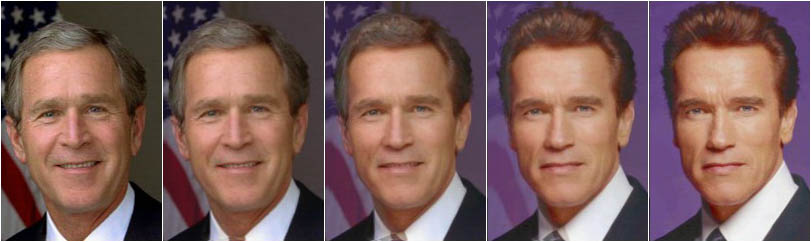
\includegraphics[scale=0.5, trim = 0 1.1cm 0 0, clip]{Pictures/Striscia_morphing.jpg}
\caption{Processo di morphing con alcuni risultati intermedi.}\label{fig:figura}
\end{figure}

\noindent
Durante la dissolvenza dall'immagine iniziale a quella finale, le immagini vengono deformate facendo in modo che ciascun punto chiave si muova lungo il percorso che porta dalla sua posizione nell'immagine di partenza alla posizione del corrispondente punto nell'immagine di arrivo.
\newpage
\chapter{Trattazione del problema}
\chapter{Equazione del calore e metodo Perona-Malik}
L'equazione del calore, come facilmente intuibile, è stata formulata per determinare l'evoluzione di un sistema isolato che presenta al suo interno una data distribuzione di calore.\\
Euristicamente, non è difficile pensare che si possano codificare (pensando ad un'immagine in bianco e nero) i pixel più luminosi come punti "più caldi", mentre quelli più scuri come punti "più freddi" ed applicare così l'equazione del calore all'immagine.\\
Mediante uno script MATLAB si può dunque osservare come quest'ultima operi nella pratica, sfruttando una approssimazione alle \textbf{differenze finite } utile per il calcolo delle derivate.\\
\section{Metodo delle differenze finite}
Il metodo delle differenze finite, come anticipato, viene impiegato nel calcolo approssimato delle derivate. Il procedimento segue dalla definizione in sè di derivata. \\La scelta adottata per la suddetta approssimazione risulterà dunque essere:\\
\vspace{2em}
\centering 
{\Large$\frac{du}{dx} \approx \frac{u_{i+1} - u_i}{\Delta(x)} $.}\\
~\\
~\\
~\\
~\\
~\\
~\\
~\\
~\\
~\\
~\\
~\\
~\\

\newpage
\raggedright
In particolare, dal momento che la derivata seconda coincide con la derivata della derivata prima, allora quest'ultima può essere approssimata nel seguente modo:\\
\centering    
{\large
\begin{align*}
\frac{d^2u}{dx^2} \approx &
\frac{
(\frac{u_{i+1} - u_i}{\Delta(x)})_{i+1} 
- 
(\frac{u_{i+1} - u_i}{\Delta(x)})_i
}{\Delta(x)}
\\
\vline
\\
= &
\frac{
\frac{(u_{i+1} - u_i)_{i+1}}{\Delta(x)} 
-   
\frac{(u_{i+1} - u_i)_i}{\Delta(x)}
}{\Delta(x)}
\\
\vline 
\\
= &
\frac{
\frac{(u_{i+2} - u_{i+1})}{\Delta(x)} 
- 
\frac{(u_{i+1} - u_i)}{\Delta(x)}
}{\Delta(x)}
\\
\vline 
\\
= &
\frac{
\frac{(u_{i+2} - u_{i+1}) 
- 
(u_{i+1} - u_i)}{\Delta(x)}
}{\Delta(x)}
\\
\vline
\\
= &
\frac{
(u_{i+2} - u_{i+1}) 
- 
(u_{i+1} - u_i)}
{\Delta(x)^2}
\\
\vline 
\\
= &
\frac{
 u_{i+2} - u_{i+1} 
-u_{i+1} + {u_i}}
{\Delta(x)^2}
.\\
\end{align*}
}
\raggedright
Per una ottenere una stima accurata, è bene utilizzare un valore di $\Delta(x)$ quanto più basso possibile. La migliore è guardare la differenza tra un pixel e quello adiacente ossia $\Delta(x)=1$, ma allora 
{\large
$$\frac{d^2u}{dx^2} \approx
\frac{
 u_{i+2} - u_{i+1} 
-u_{i+1} + u_i}
{\Delta(x)^2} = u_{i+2} -2 u_{i+1} + u_i.$$
}
\`E chiaro che scorrendo tutti gli indici questo è equivalente a $u_{i+1} -2 u_i + u_{i-1}.$

In sintesi si può utilizzare per il calcolo del laplaciamo l'approssimazione \\
\vspace{2pt}
\centering 
{\Large
$\frac{d^2u}{dx^2} \approx u_{i+1} -2 u_i + u_{i-1}$.\\
}
\vspace{2pt}
\raggedright
\newpage
\subsection{Errore di troncamento}

Vale la pena di fare qualche considerazione sull'errore di troncamento che si commette adottando queste approssimazioni.\\
Per definizione, l'errore è la differenza tra il valore esatto e quello approssimato, ossia: 

$$
\frac{d^2u}{dx^2}\vline_{x_i}-\frac{u_{i+1}-u_i}{\Delta(x)}\approx \frac{\Delta(x)^2}{2} \frac{d^2u}{dx^2}\vline_\xi.
$$

Risulta quindi evidente che l'errore dipende da $\Delta(x)^2$. 
Ad un'attenta analisi possiamo vedere che tra i metodi di approssimazione in avanti, in indietro o centrale, il calcolo dell'errore portato dai primi due sono uguali tra di loro, quello centrale invece è diverso, esso dipende da un $\Delta(x)^3$ e non da un $\Delta(x)^2$, questo vuol dire che per $\Delta(x)<1$ funziona meglio, per $\Delta(x)>1$ funziona peggio. Nel caso in analisi $\Delta(x)=1$ quindi la scelta è indifferente.
%Ma procediamo con ordine.\\

Per brevità di notazione poniamo $\Delta(x)=h$.\\
Dagli sviluppi di Taylor in $x_j$ di
$u(x_{j \pm 1}) = u(x_j \pm h)$ fino al terzo ordine, si ottiene che

$$
u''(x_j) =\frac{u(x_{j+1}) - 2u(x_j) + u(x_{j-1})}{h^2} -\frac{1}{12} u^{(4)}(\xi_j)h^2
$$

dove $\xi_j$ e un punto opportuno in $(x_{j-1} , x{j+1})$. Quindi, considerando il problema modello con condizoni di Dirichlet, per $j = 1,...,N-1$, si può scrivere che

$$
\frac{-u(x_{j+1}) + 2u(x_j) -u(x{j-1})}{h^2}
 + \frac{1}{12} u^{(4)}(\xi_j)h^2 + \sigma(x_j)u(x_j) = f(x_j) .
$$

Introducendo la notazione $\tau_{j}=\frac{1}{12} u(4)(\xi_j)h^2$ (errore di troncamento locale) e ponendo:\\

$\boldsymbol{u}=[u_x...u_{N-1}]^T$\\
$\boldsymbol{\tau_h}=[\tau_x...\tau_{N-1}]^T$\\
$\boldsymbol{b_h}=[(f(x_1) + \frac{g_0}{h^2},f(x_2),...,f(x_{N-2}),f(x_{N-1}) + \frac{g_1}{h^2}]^T$\\

si può allora scrivere in forma matriciale,
$A_h\boldsymbol{u} = \boldsymbol{b_h} + \boldsymbol{\tau_h}$
dove $A_h = \frac{1}{h^2}
 tridiag(-1,2,-1) + diag(\sigma_1, ... ,\sigma_{N-1}) e \sigma_j = \sigma(x_j)$.\\
\vspace{1em}
Il metodo alle differenze finite consiste allora nel determinare un’approssimazione $u_h$ di
u andando a risolvere il sistema lineare
$A_h\boldsymbol{u_h} = \boldsymbol{b_h}.$
Osserviamo che $\boldsymbol{u_h}$ risulta ben definito in quanto $A_h$ è una matrice non singolare.\\

\vspace{1em}

Risultando che $\boldsymbol{\tau_h}$ tende a zero quando h tende a zero, il metodo dicesi consistente. In particolare nel caso in analisi, come osservato in partenza, risulta $\boldsymbol{\tau_h} = O(h^2)$ .\\
Tuttavia la consistenza non assicura da sola la convergenza del metodo.\\
Per studiarne laconvergenza è necessario considerare il comportamento dell’errore $\boldsymbol{e_h} = \boldsymbol{u_h} -\boldsymbol{u}$ quando h tende a zero. Dato che risulta $A_h\boldsymbol{e_h} = \boldsymbol{\tau_h}$, e quindi $\boldsymbol{e_h} = A_h^{-1} \boldsymbol{\tau_h}$ si può quindi scrivere: $||\boldsymbol{e_h}||\geq ||A_h^{-1}|| |\boldsymbol{\tau_h}||$\\
Il passaggio successiovo è far vedere che, lavorando in norma infinito, si è in grado di trovare una costante che, per ogni $h$, maggiora $||A_h^{-1}||$. \\ 
\newpage
A questo scopo osservando che si può dimostrare che sia $A_h$ che la matrice $A_{0h} = \frac{1}{h^2} tridiag(-1,2,-1)$ hanno inversa non negativa, e si ha: 

$$A_{0h}^{-1}-A{h}^{-1}=A_{0h}^{-1}(A_h-A_{0h})A_h^{-1}\geq0.$$

Per le ipotesi su $\sigma$ questo implica $A_h^{-1}||\leq A_{0h}^{-1}||$
osserviamo che
$||A_{0h}^{-1}||=max_j(A_{0h}^{-1}\boldsymbol{e})_j$ dove $\boldsymbol{e}$ indica il vettore di tutti 1.\\
Osservando che la soluzione esatta del problema $-u'' = 1, u(0) = u(1) = 0$, è il polinomio di secondo grado $\phi(x) = \frac{x(1-x)}{2}$, si può concludere che $A_{0h}^{-1}\boldsymbol{e})_j=\phi(x_j)$ e quindi che $A_h^{-1}||\leq A_{0h}^{-1}||\leq max_{0<x<1}|\phi_x|$.\\
Questo risultato di stabilità ci permette di concludere che l’errore $\boldsymbol{e_h}$ ha lo stesso ordine dell’errore di troncamento $\boldsymbol{\tau_h}$ e di conseguenza che il metodo è convergente del secondo ordine.
Si noti che l’uniforme limitatezza della norma di $A_h^{-1}$ implica che il metodo numerico sia stabile. 




\newpage

\section{L'equazione del calore}

\raggedright

Il metodo delle differenze finite sarà impiegato in uno script MATLAB per l'implementazione dell'equazione del calore, è bene quindi prenderla in esame.

\begin{equation} 
\begin{cases}

\frac{\partial u}{\partial t}(t,x)-\Delta u(t,x) = 0 \ x \in \mathbb R^2, t\ge 0 \ .\\ 

u(0,x) = u_0(x)\ . \\

\end{cases}
\end{equation}

L'equazione del calore, come anticipato, determina l'evoluzione di un sistema isolato che presenta al suo interno una data distribuzione di calore. \`E banale pensare che con il passare del tempo il calore si distribuisca, tendendo per un tempo infinito ad una distribuzione uniforme.

\vspace{1em}

Applicando l'equazione del calore si ottiene quindi un'immagine sempre più "liscia", di fatto una sfocatura, e per un numero di iterazioni idealmente infinito si giungerebbe ad una distribuzione uniforme di colore, ossia una tinta unita.

\vspace{1em}
%\newpage

Il seguente script MATLAB illustra come questo processo opera nella pratica.

\begin{lstlisting}[language=MATLAB]
Im=imread('parrot.jpeg');   %Apro l'immmagine
Im=rgb2gray(Im);            %La trasformo in bianco e nero
Im = imnoise(Im,'gaussian');%Aggiungo del rumore

%---Definisco le costanti e le condizioni iniziali

[ny, nx, ~]=size(Im)        %Dimensioni dell'immagine
dt=0.25;                    %Passo temporale
u=double(Im);               %Copia dell'immagine originale su cui                                lavorare
T=3			                    %Tempo, ossia T/dt + 1 definisce il numero                            di iterazioni da eseguire
k=0.5;

%---Mostro l'immagine originale
imshow(uint8(Im))
title('immagine originale'); 

%---Metodo eq del calore
u=double(Im);
for t = 0:dt:T
   u_xx = u(:,[2:nx nx],:) - 2*u + u(:,[1 1:nx-1],:);  % derivata                                                           seconda lungo x
   u_yy = u([2:ny ny],:,:) - 2*u + u([1 1:ny-1],:,:);  % derivata                                                            seconda lungo y
   u= u + k*dt*(u_xx+u_yy);
   temp=u;
end

\end{lstlisting}
%\vspace{1em}
\newpage
Provando a cambiare il tempo, ossia il numero di iterazioni, si può osservare come un maggior lasso di tempo produca immagini più sfocate.

\begin{figure}[h!] 
\centering
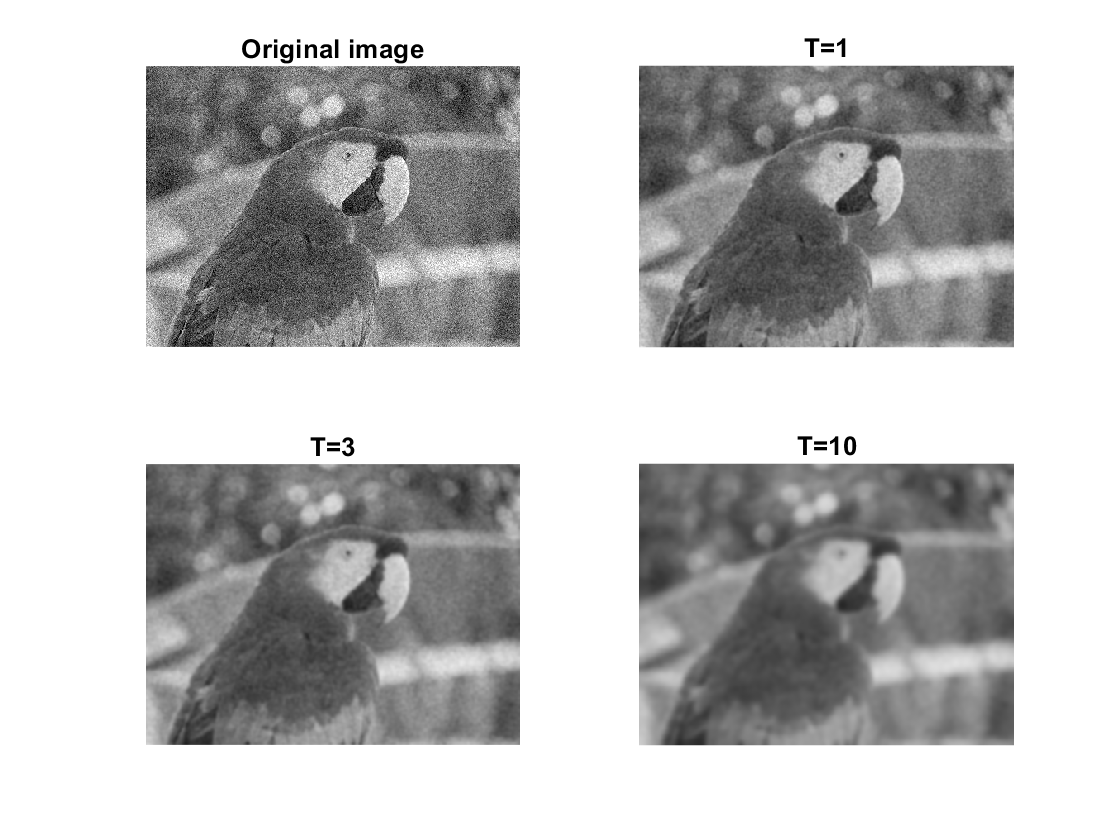
\includegraphics[scale=0.27, trim = 0 12.3cm 1.9cm 1.9cm, clip]{Pictures/Risultati/eq del calore.png}
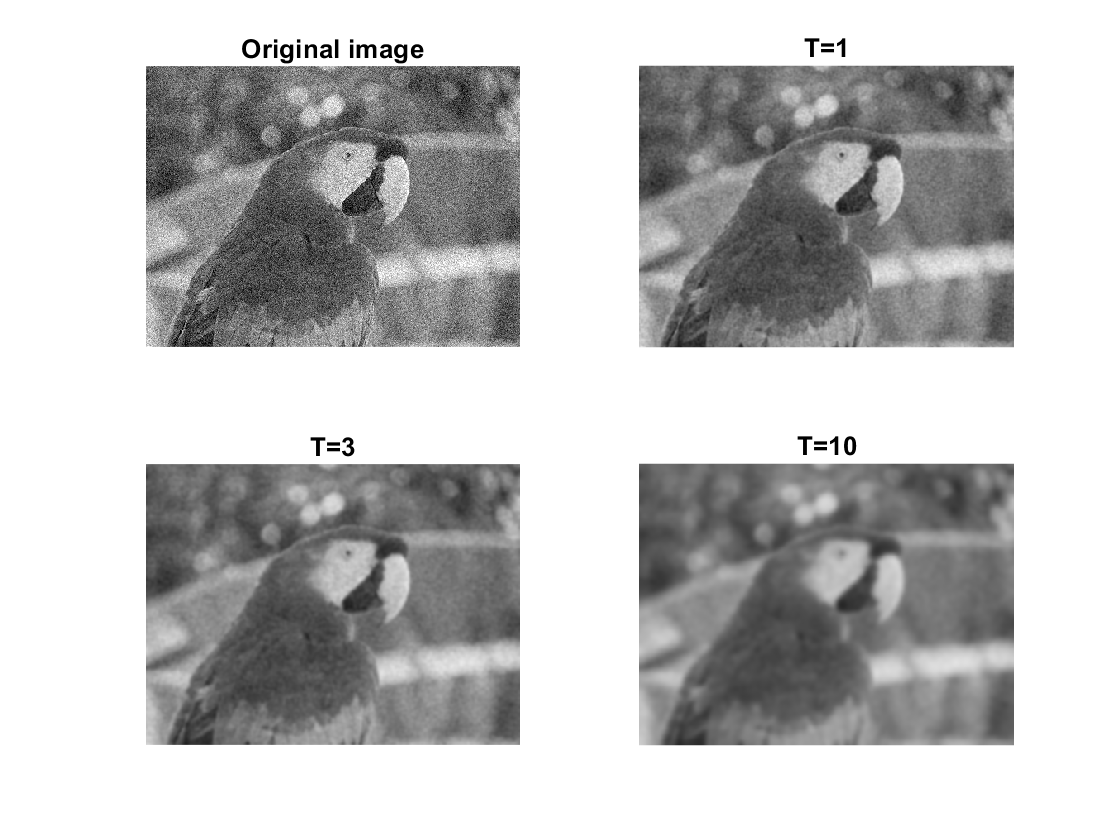
\includegraphics[scale=0.27, trim = 1.9cm 1.7cm 1.9cm 10.3cm, clip]{Pictures/Risultati/eq del calore.png}
\caption{Effetti dell'equazione del calore nel tempo.}\label{fig:figura}
\end{figure}


Questo metodo però non è poi molto utile in generale, sì, il rumore viene eliminato o almeno ridotto ma si perdono importanti dettagli, esistono procedimenti come il metodo Perona-Malik che sono decisamente più utili.\\
L'idea del metodo Perona-Malik è di applicare l'equazione del calore nelle regioni in cui il colore è più uniforme, così da preservarne i bordi.



\section{Rilevamento dei bordi}

Operando una derivata in una data direzione, per il significato in sè di derivata, questa assume valori più elevati quando la variazione è elevata, e assume valori nulli quando non c'è variazione in quella direzione. Per questo motivo, applicata ad un' immagine, ne rileviamo i bordi!\\
Presa una tinta unita la derivata sarà quindi nulla in ogni suo punto (è intuitivo: se un'immagine è una funzione che, date due coordinate restituisce un colore, allora una tinta unita è una funzione costante ed in quanto tale ha derivata nulla).\\
\vspace{1em}
Operando una derivata seconda in una data direzione, per il significato in sè di derivata seconda, questa assume valori più elevati quando la concavità è più stretta, e assume valori pressocchè nulli quando non ci sono concavità (si può pensare alle concavità come a dei picchi o dei ventri, su di una immagine vuol dire chiazze di colore diverso).\\
Presa una sfumatura di colore che varia in maniera lineare, la derivata seconda sarà nulla in ogni suo punto, la derivata prima sarà invece costante. 
\newpage
Si riporta un piccolo script MATLAB che mette in evidenza questo aspetto.
\vspace{1em}
\begin{lstlisting}[language=MATLAB]
%---Operazioni preliminari
Im=imread("nome_immagine.png");	%Apro l'immmagine

[ny, nx, ~]=size(Im)        %Memorizzo le dimensioni dell'immagine
u=double(Im);               %Copia dell'immagine originale su cui lavorare
h=80;                       %Definisco un parametro che usero' per                               enfatizzare i bordi in fase di stampa 


%---Calcolo tutte le derivate
u_x =  u(:,[1 1:nx-1],:) - u;                       %derivata                                                            prima lungo x
u_xx = u(:,[2:nx nx],:) - 2*u + u(:,[1 1:nx-1],:);  %derivata                                                            seconda lungo x
u_y =  u([1 1:ny-1],:,:) - u;                       %derivata                                                            prima lungo y
u_yy = u([2:ny ny],:,:) - 2*u + u([1 1:ny-1],:,:);  %derivata                                                            seconda lungo y
u_xy = u_x([1 1:ny-1],:,:) - u_x;                   %derivata                                                            seconda mista
   
%---Stampo i risultati
figure()
subplot(2,3,2),text(0.3,0,nome,'FontSize',20); axis off
subplot(2,3,4), imshow(Im)
title('Immagine originale')
subplot(2,3,5), imshow(uint8(h*abs(u_x)))
title('h*u_x')
subplot(2,3,6), imshow(uint8(h*abs(u_y)))
title('h*u_y')

figure()
subplot(2,3,2),text(0.3,0,nome,'FontSize',20); axis off
subplot(2,3,4), imshow(Im)
title('Immagine originale')
subplot(2,3,5), imshow(uint8(h*abs(u_x + u_y)))
title('h*(u_x + u_y)')
subplot(2,3,6), imshow(uint8(h*abs(u_xx + u_yy)))
title('h*(u_xx + u_yy)')
\end{lstlisting}

\vspace{1em}
Lo script permette di osservare come con diverse immagini molto semplici se otteniamo i risultati attesi.\\
%\vspace{1em}
\newpage
\begin{figure}[htb] 
\centering
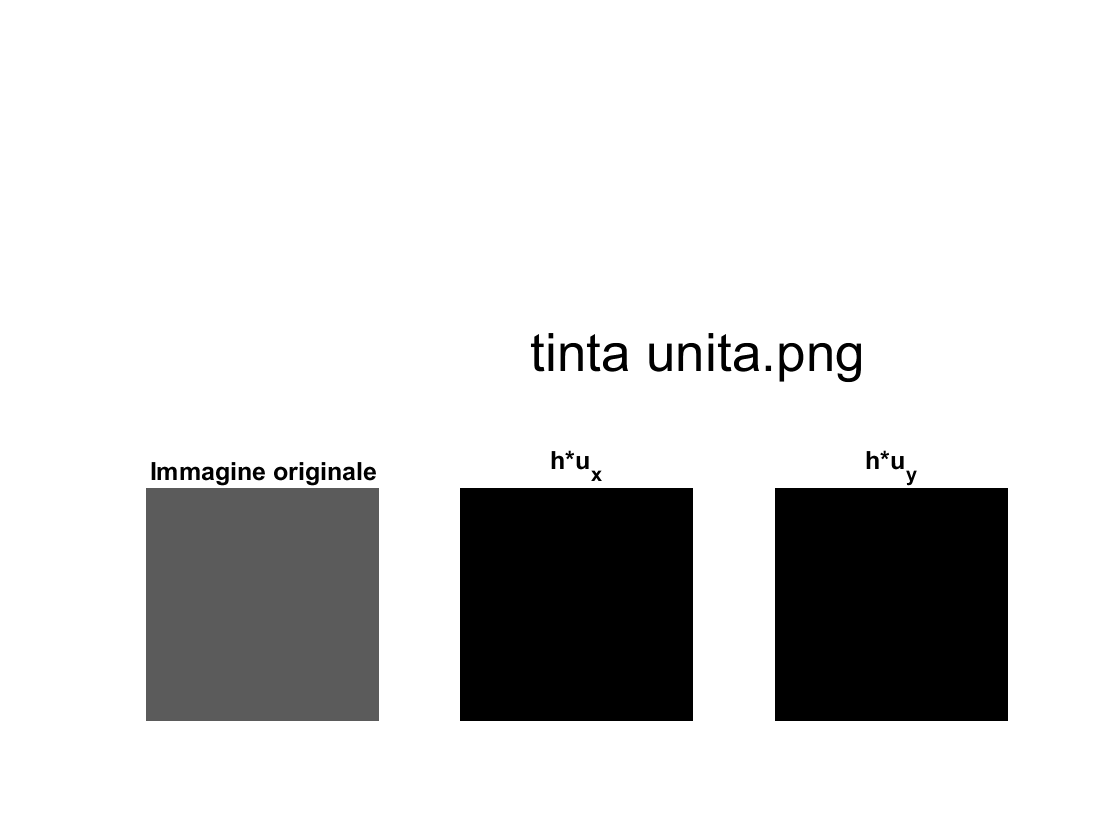
\includegraphics[scale=0.4, trim = 0 0 0 10.5cm, clip]{Pictures/Risultati/tinta unita bianco e nero derivate parziali.png}
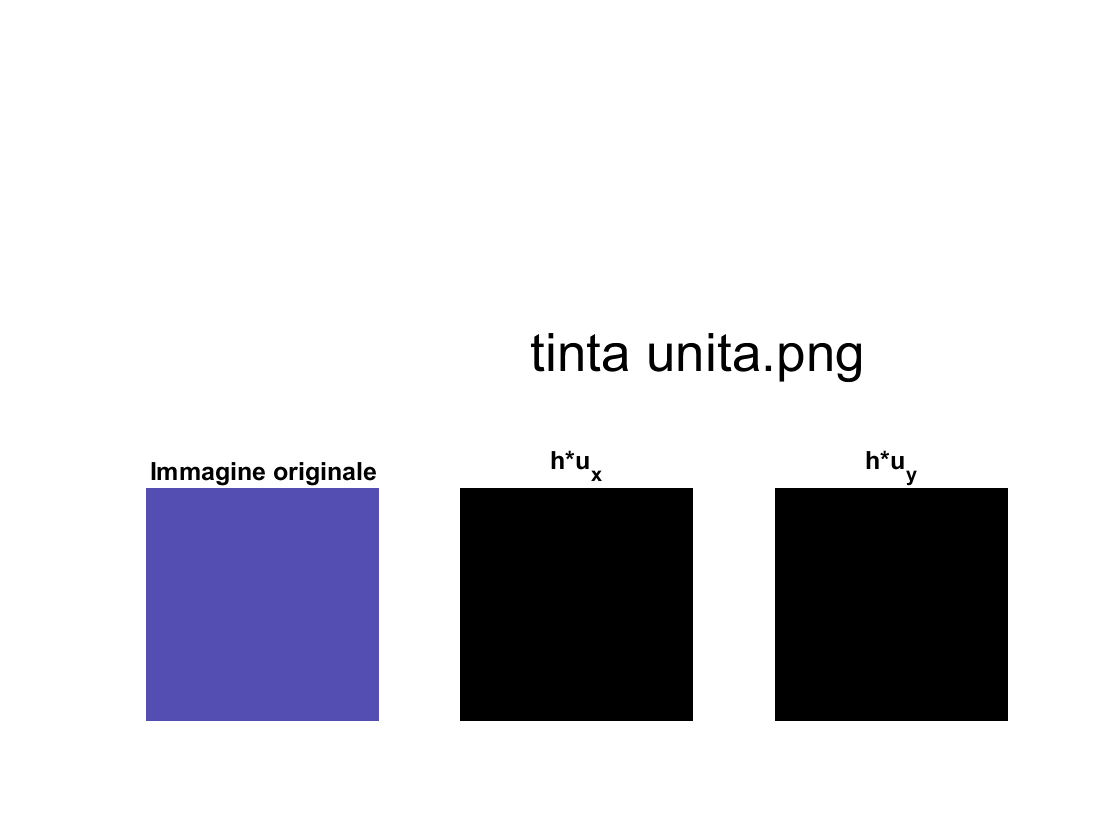
\includegraphics[scale=0.4, trim = 0 0 0 10.5cm, clip]{Pictures/Risultati/tinta unita derivate parziali.png}
\caption{Derivate parziali di una tinta unita.}\label{fig:figura}
\end{figure}

Si può vedere come con un'immagine a tinta unita (che sia essa in bianco e nero o a colori) le derivate sono nulle, quindi lo saranno anche gradiente e laplaciano. Confermiamo inoltre che questi principi valgono sia a colori che in bianco e nero.\\

\newpage
\begin{figure}[htb] 
\centering
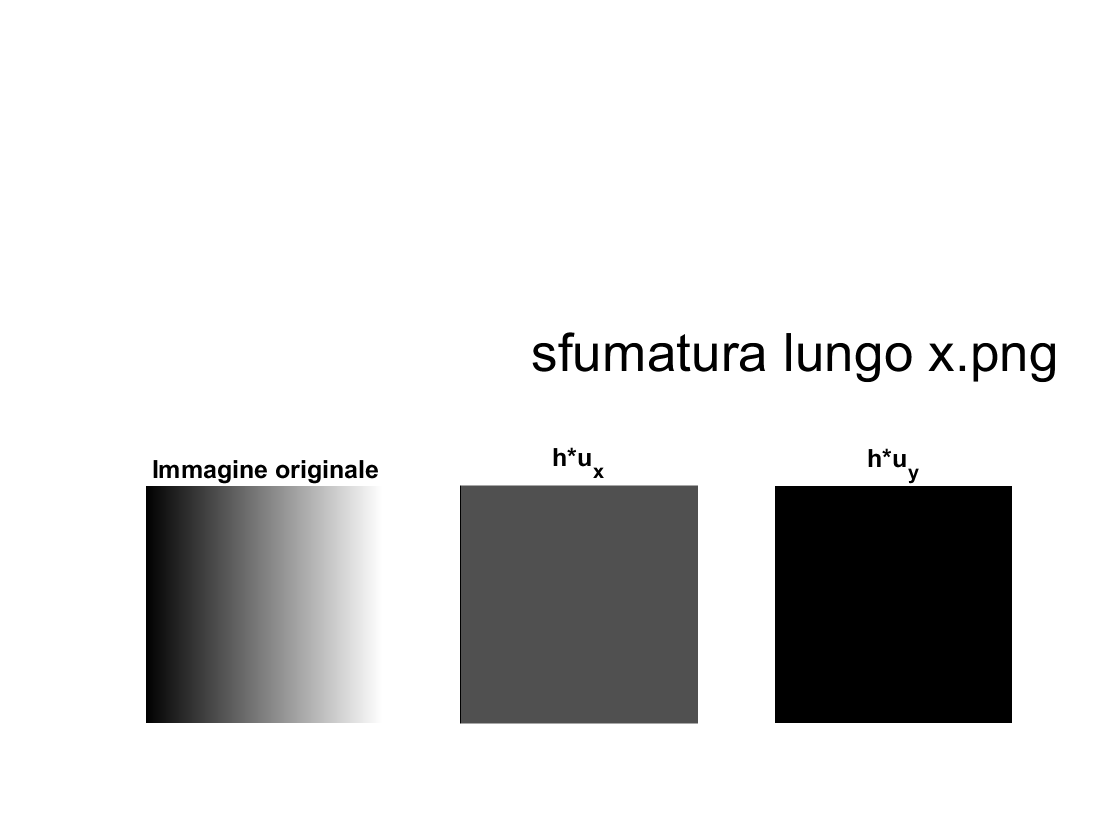
\includegraphics[scale=0.4, trim = 0 0 0 10.5cm, clip]{Pictures/Risultati/sfumatura lungo x bianco e nero derivate parziali.png}
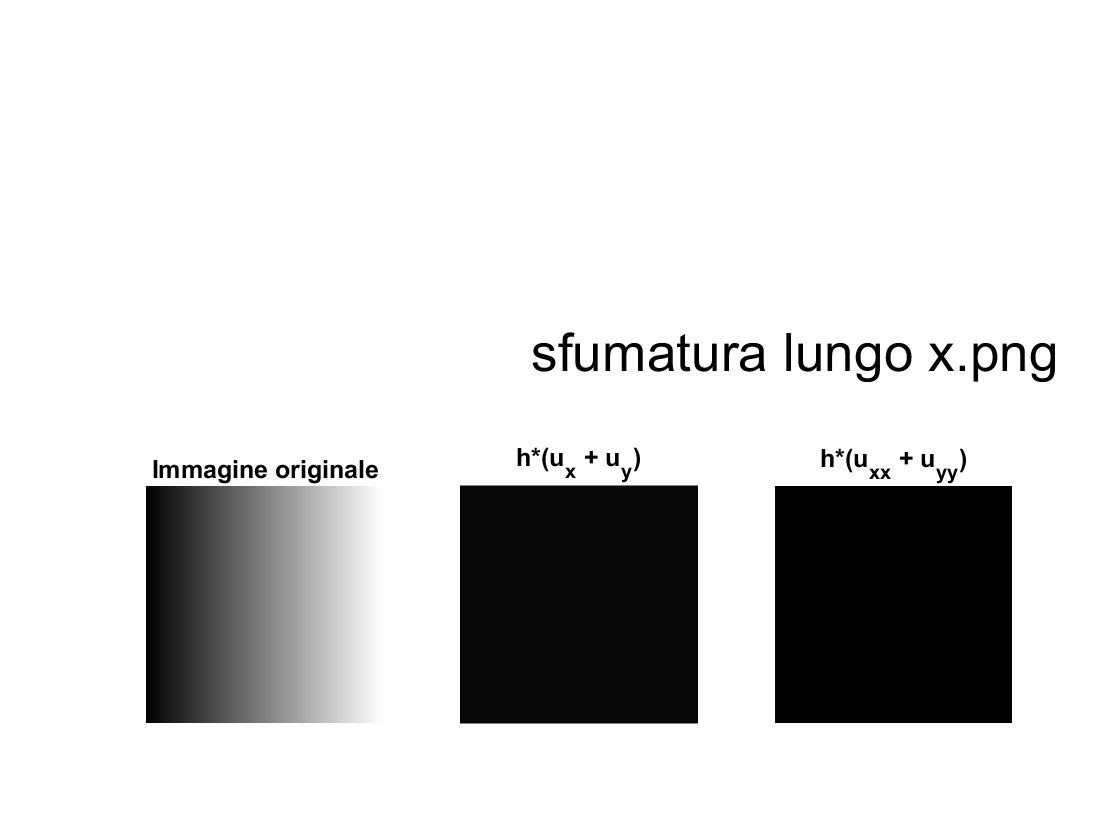
\includegraphics[scale=0.4, trim = 0 0 0 10.5cm, clip]{Pictures/Risultati/sfumatura lungo x bianco e nero gradiente e laplaciano.png}
\caption{Derivate parziali, gradiente e laplaciano di una sfumatura orizzontale.}\label{fig:figura}
\end{figure}

Guardando invece ad una immagine che presenta una sfumatura lineare lungo l'asse x, la derivata lungo x assume un valore costante mentre la derivata lungo y è nulla, proprio perchè lungo y non c'è variazione mentre lungo x c'è una variazione costante.\\
Ovviamente, date queste premesse, il gradiente sarà costante uguale ad $u_x$ (siccome $u_y=0$) e quindi il laplaciano sarà nullo.
Il fatto che in entrambi questi esempi il laplaciano sia nullo è un buon segno, lo useremo per rilevare i bordi ed in queste immagini non ve ne sono, quindi è giusto che il laplaciano sia nullo.\\

\newpage
\begin{figure}   
\centering
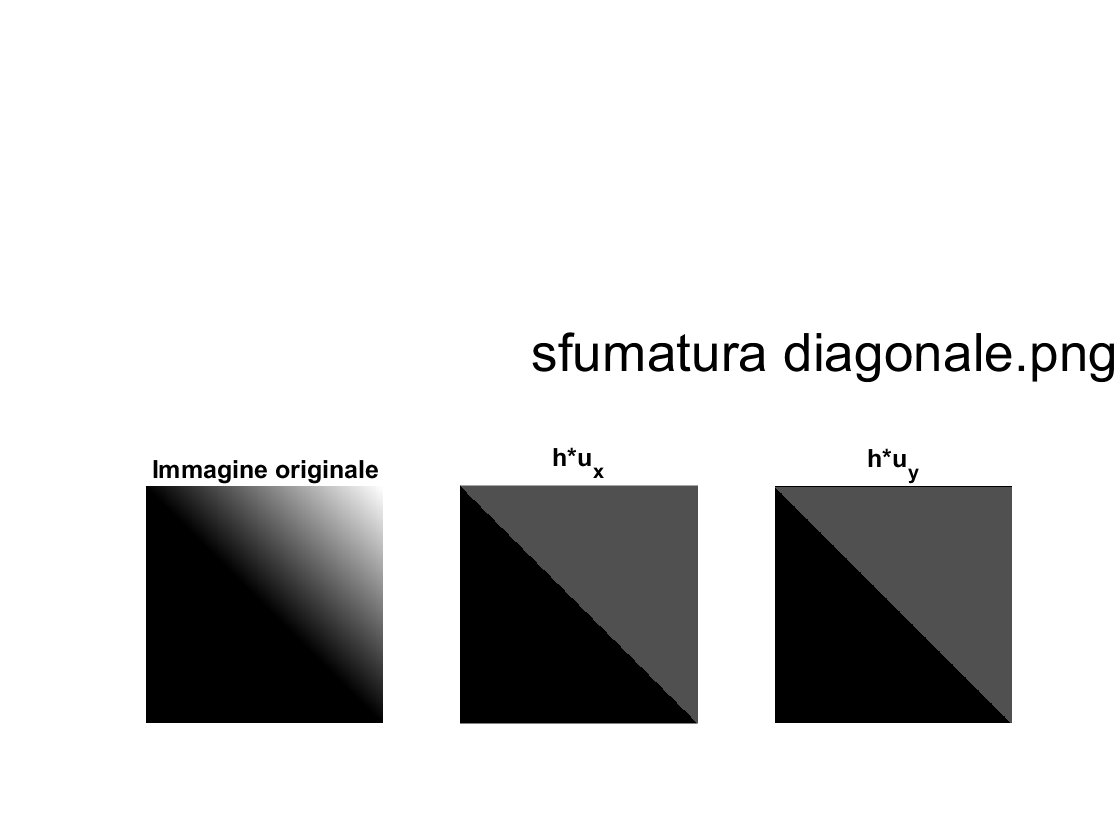
\includegraphics[scale=0.4, trim = 0 0 0 10.5cm, clip]{Pictures/Risultati/sfumatura diagonale bianco e nero derivate parziali.png}
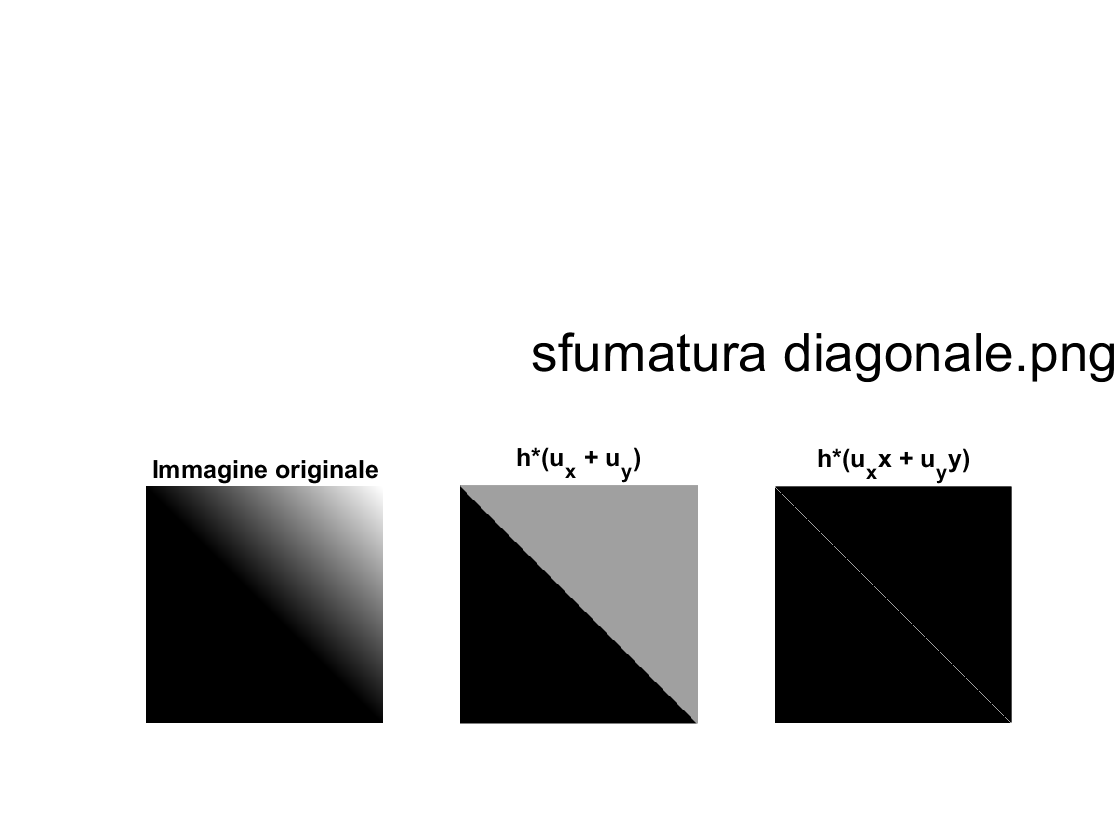
\includegraphics[scale=0.4, trim = 0 0 0 10.5cm, clip]{Pictures/Risultati/sfumatura diagonale bianco e nero gradiente e laplaciano.png}
\caption{Derivate parziali, gradiente e laplaciano di una sfumatura diagonale.}\label{fig:figura}
\end{figure}

Presa una sfumatura diagonale, ma solo su metà immagine vediamo dei riultati interessanti: entrambe le derivate parziali sono nulle nelle regioni in cui non c'è sfumatura, esattamente come nel caso della tinta unita, ed entrambe sono costanti dove c'è sfumatura (che ricordiamo essere lineare).\\
Tutto ciò riconferma quanto visto dai punti precedenti, volgendo quindi uno sguardo al gradiente ed al laplaciano si può notare che mentre il gradiente ha un aspetto molto simile alle due derivate parziali, sommando i loro valori è semplicemente più luminoso, per quanto riguarda il lplaciano la storia cambia. Le derivate seconde sono indicatrici della variazione delle derivate prime, cioè della variazione della variazione del valore della funzione, ma l'unica variazione che hanno le derivate prime è lungo la diagonale.
Abbiamo così individuato il nostro primo bordo, cioè la diagonale che divide di fatto due regioni, una in cui il colore è costante ed una in cui sfuma.\\

\vspace{1em}

Si riporta un ultimo esempio, provando ad introdurre una semplice figura e osserviamo cosa accade.\\

\newpage
\begin{figure}[htb] 
\centering
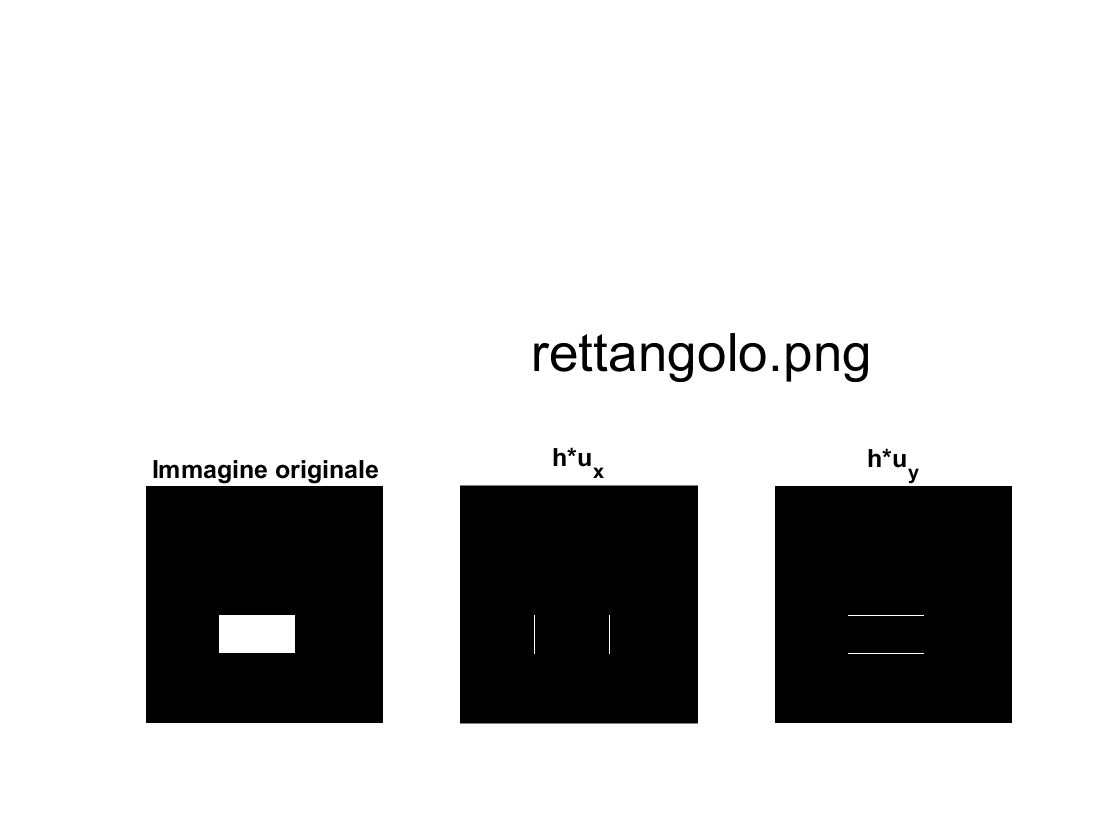
\includegraphics[scale=0.4, trim = 0 0 0 10.5cm, clip]{Pictures/Risultati/rettangolo bianco e nero derivate parziali.png}
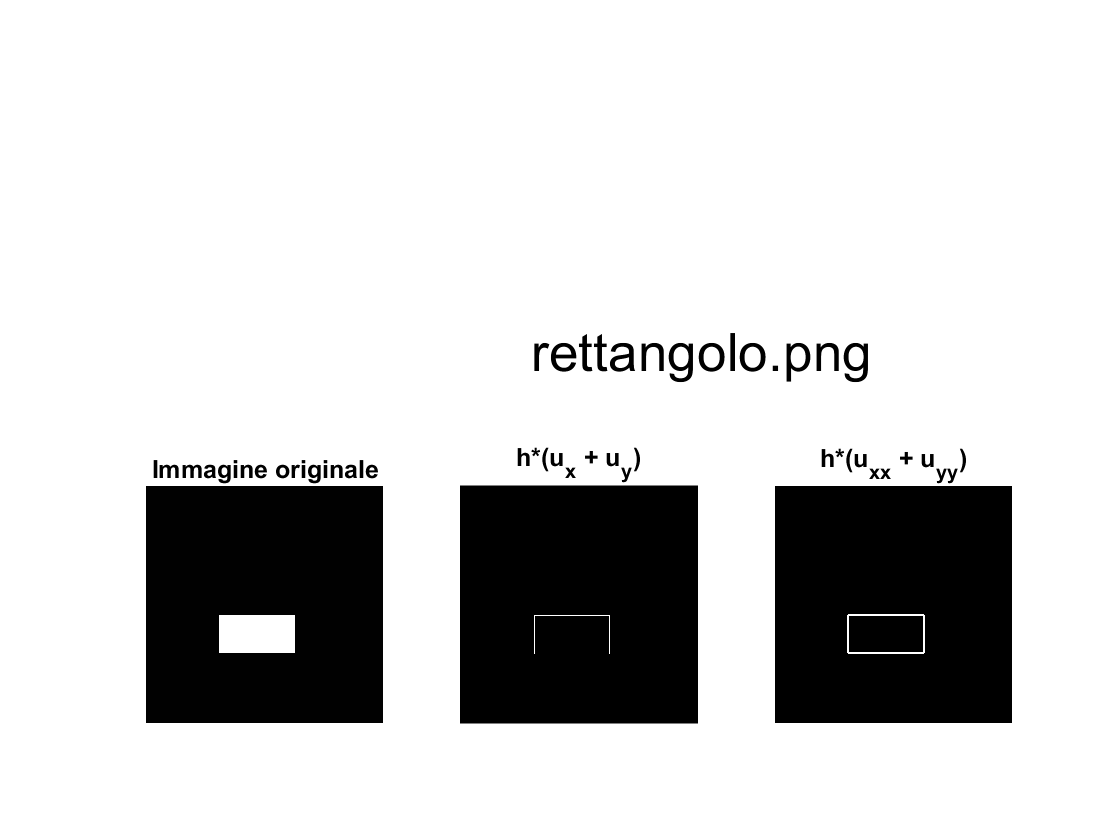
\includegraphics[scale=0.4, trim = 0 0 0 10.5cm, clip]{Pictures/Risultati/rettangolo bianco e nero gradiente e laplaciano.png}
\caption{Derivate parziali, gradiente e laplaciano di una figura semplice.}\label{fig:figura}
\end{figure}

Importando un rettangolo nero su di uno sfondo bianco, come confermato anche dalla prima sfumatura, la derivata lungo x rileva i bordi verticali, quella lungo y i bordi orizzontali, dalla loro somma (quindi dal gradiente) otteniamo già il bordo del rettangolo.
Il bordo così ottenuto è un bordo che idealmente rimarrà inalterato a prescindere dall'ordine della derivata, in particolare quindi anche per derivate seconde, quindi il laplaciano continua a soddisfare la richiesta di determinare i bordi. \\
Come detto: "Il bordo così ottenuto è un bordo che idealmente rimarrà inalterato a prescindere dall'ordine della derivata" è interessante capire perchè. Presa una striscia di pixel, cioè uno strato dell'immagine (la si può immaginare quindi come una funzione da R in R), risulterà essa raffigurare una funzione porta!\\
La funzione porta non è derivabile in senso classico, ripensando alla definizione di derivata avremmo un valore di +infinito prima e -infinito poi. La sua derivata sarà quindi una coppia di delta di Dirac.\\


\newpage
\section{Metodo Perona-Malik}

Il metodo Perona-Malik, come anticipato, si basa sull'equazione del calore. L'idea è quella di applicare tale equazione lontano dai bordi dell'immagine e mantenere invece inalterati quest'ultimi.
Questo metodo risulta particolarmente efficace per risolvere problemi di disturbo come ad esempio un rumore del tipo salt and pepper, cioè con dei pixel bianchi o neri sparsi per la foto.\\
\vspace{1em}
\`E bene capire da un punto di vista prettamente matematico cosa vuol dire che il metodo si basa sull'equazione del calore, che ricordiamo essere:\\
$$
\begin{cases}
\frac{\partial u}{\partial t}(t,x)-\Delta u(t,x) = 0 \ x \in \mathbb R^2, t\ge 0 \ .\\ 
u(0,x) = u_0(x)\ . \\
\end{cases}
$$
Il laplaciano è la divergenza del gradiente, ed è qui che viene operata la modifica.\\
Come detto: $\Delta(u)=div(\nabla(u))$, volendo operare un controllo si introdurrà un coefficiente $k$ ottenendo $div(k\nabla(u))$, nel caso esso sia uno scalare costante, avremo $div(k\nabla(u))=kdiv(\nabla(u))=k\Delta(u)$ ed è il caso implementato nelle pagine precedenti. Il metodo Perona-Malik invece prevede l'impiego di un coefficiente k non costante, ma che cambi a seconda del pixel su cui si opera, otteniamo così una matrice delle stesse dimensioni della matrice che rappresenta l'immagine e che funga da mappa, indicante per ogni pixel l'intensità con cui la diffusione va applicata. In questo senso, questo filtro viene detto di diffusione anisotropa.
Il termine diffusione anisotropa indica, a livello globale, quella particolare proprietà secondo cui la diffusione del colore sull'immagine dipende fortemente dalla direzione presa in considerazione. Tuttavia è possibile constatare come questa dicitura sia in realtà un abuso di notazione di cui ci serviamo in termini prettamente esplicativi dal momento che il metodo in esame è localmente isotropo, si articola cioè lungo un’unica direzione variandone però l’intensità punto per punto.
%Il termine anisotropo indica come la diffusione sia diversa nelle varie direzioni, capiamo quindi come questa notazione, per quanto esplicativa sia in verità un abuso di notazione siccome la diffusione non avviene in direzioni diverse ma semplicemente con intensità diverse.
Esistono tuttavia dei metodi metodi di diffusione anisotropa, in tal caso k sarà un tensore variabile.\\
\vspace{1em}
Ritornando al metodo in esame, il problema affrontato diventa\\
$$
\begin{cases}
\frac{\partial u}{\partial t}(t,x)-div(k\nabla(u)) = 0 \ x \in \mathbb R^2, t\ge 0 \ .\\ 
\frac{\partial u}{\partial N}=0 \ x \in \mathbb R^2, t\ge 0 \ .\\ 
u(0,x) = u_0(x)\ . \\
\end{cases}
$$
Con k dipendente dal gradiente, in particolare $k=k(|\nabla(u)|^2)$.

Servirà dunque esplicitare e discretizzare questo problema, per fare ciò saranno impiegati, oltre ai metodi già visti, altri accorgimenti.\\

\newpage
\subsection{Soluzione discreta della PDE}
Sia u una funzione, sia $D_f(x_i)$ la differenza finita in avanti, $D_b(x_i)$ la differenza finita all'indietro e sia $D_c(x_i)$ la differenza finita centrata, si può osservare che:
$$
D_f(x_i)+D_b(x_i)= \frac{u_{i+1} - u_{i}}{\Delta(x)} + \frac{u_{i} - u_{i-1}}{\Delta(x)} = \frac{u_{i+1} - u_{i-1}}{\Delta(x)} = 2D_c(x_i)
$$
Capiamo quindi che la differenza finita centrata è $D_c(x_i)=\frac{1}{2}(D_f(x_i)+D_b(x_i))$ cioè la media delle altre due.\\ Preso un punto si può operare le differenze finite nelle 4 direzioni, le indicheremo con N (Nord), S (Sud), W (Ovest) e E (Est). Notiamo allora che la differenza finita Nord è la differenza finita in avanti rispetto a y, mentre la differenza finita S è la differenza finita all'indietro rispetto a y, la loro media sarà quindi la differenza finita centrata rispetto a y. Analogamente la media delle differenze finite Ovest ed Est sarà la differenza finita centrata rispetto a x. In formule:\\
%\vspace{-1em}
$$
\frac{\partial u}{\partial x} \approx \frac{u_E+u_W}{2} \hspace{1em};\hspace{1em}
\frac{\partial u}{\partial y} \approx \frac{u_N+u_S}{2}
$$
Ricordiamo che il gradiente è il vettore delle derivate parziali, la divergenza invece è la somma delle derivate parziali.
Calcoliamo quindi un'approssimazione discreta della PDE\\
%\vspace{-1em}


\begin{align*}
    \frac{\partial u}{\partial t}(t,x)&=div(k\nabla(u))=\\
    &=\frac{k\nabla u}{\partial x} +\frac{k\nabla u}{\partial y}\\
    &\approx\frac{k_N\nabla_N + k_S\nabla_S}{2} +\frac{k_W\nabla_W + k_E\nabla_E}{2}\\
    &=\frac{1}{2}(k_N\nabla_N + k_S\nabla_S k_W\nabla_W + k_E\nabla_E) 
\end{align*}


Ci si ritrova quindi a risolvere l'equazione 
$$
\frac{\partial u}{\partial t}(t,x)=\frac{1}{2}(k_N\nabla_N + k_S\nabla_S k_W\nabla_W + k_E\nabla_E) 
$$
che è della forma $y'(x)=f(x,y(x))$ e può quindi essere risolta con un metodo semplice.
Ancora una volta ricorriamo alle differenze finite.
$$
y'(x_i)\approx \frac{y(x_{i+1})-y(x_{i})}{\Delta t} 
$$
ma $y'(x)=f(x,y(x))$ questo vuol dire che
$$
\frac{y(x_{i+1})-y(x_{i})}{\Delta t}\approx f(x,y(x)) \Rightarrow y_{i+1} \approx y_{i} + \Delta t f(x,y(x))
$$
tale metodo è detto \textbf{metodo di Eulero esplicito}\footnote{\cite{monegato}}

La soluzione discreta della PDE, con il metodo di Eulero esplicito, sarà quindi:\\

$$
u_{i+1} = u_i + dt\frac{1}{2}(k_N\nabla_N + k_S\nabla_S + k_W\nabla_W + k_E\nabla_E)
$$

%\subsubsection{Stabilità del metodo}
\begin{osservazione}
Tramite il metodo di Von Neuman, in modo simile a quanto fatto per l'equazione del calore si
dimostra che il metodo Perona-Malik risulta essere\\
\vspace{0.25em}
stabile $\Longleftrightarrow 4\frac{1}{2}\frac{dt}{\Delta x^2}\leq\frac{1}{2}$.\\
\vspace{0.25em}
Ricordiamo che nel caso in esame, ove $\Delta x=1$, la condizione diventa:
$$
dt\leq \frac{1}{4}.
$$
\end{osservazione}


\subsection{Maschere di convoluzione}
Per implementare il filtro di diffusione anisotropica detto \textit{Perona-Malik}, ci serviremo di alcune \textbf{maschere}.\\
Un filtro è una funzione $F:\mathbb R^2\to\mathbb R$,
%in quanto tale avrà un nucleo $\operatorname{Ker}(F):=\{v \in \mathbb R^2: Fv=0\}$ che 
in particolare è un polinomio a due incognite che, date in input delle coordinate restituirà un valore numerico, chiameremo tale coefficiente \textbf{peso}. Compiliamo quindi una maschera con i pesi calcolati in tal modo per ogni posizione ottenendo una cosa del tipo:

\begin{figure}[]
    \centering
    \begin{tabular}{|p{1.6cm}|p{1.6cm}|p{1.6cm}|}
        \hline
        \makebox[1.6cm][c]{
        \rule[-8mm]{0cm}{1.6cm}
        $a_1$} & 
        \makebox[1.6cm][c]{
        $a_2$} & 
        \makebox[1.6cm][c]{
        $a_3$} \\
        \hline
        \makebox[1.6cm][c]{
        \rule[-8mm]{0cm}{1.6cm}
        $a_4$} & 
        \makebox[1.6cm][c]{
        $a_5$} & 
        \makebox[1.6cm][c]{
        $a_6$} \\
        \hline
        \makebox[1.6cm][c]{
        \rule[-8mm]{0cm}{1.6cm}
        $a_7$} & 
        \makebox[1.6cm][c]{
        $a_8$} & 
        \makebox[1.6cm][c]{
        $a_9$} \\
        \hline
    \end{tabular}
    \caption{Esempio di maschera di convoluzione 3x3}
    \label{fig:my_label}
\end{figure}
Le dimensioni della maschera possono variare a discrezione del programmatore ma, solitamente si utilizzano maschere dimensioni piccole e dispari. Dispari perchè è importante individuare il centro della maschera. Piccole perchè l'utilizzo delle maschere porta degli effetti bordo che è bene limitare. Queste motivazioni verranno meglio spiegate a breve.\\
\vspace{1em}
Come detto nelle nozioni introduttive, applicare un filtro vuol dire operare una convoluzione tra due funzioni: l'immagine ed il filtro stesso.\\
Le maschere sono un utile strumento proprio per il calcolo delle convoluzioni, motivo per cui sono solitamente dette \textbf{maschere di convoluzione}.\\
Per operare una convoluzione, detti $u:\mathbb R^2\to\mathbb R$ l'immagine e $F:\mathbb R^2\to\mathbb R$ il filtro, per definizione, $\forall p_{i,j}\in dom(u)$ si prende un intorno $I(p)$, le cui dimensioni dipendono da quelle della maschera scelta per F. Successivamente si sommano i prodotti tra i valori di u e quelli di F, cioè i pesi della maschera, per ottenere in fine l'immagine filtrata.\\
\vspace{1em}
In pratica, si scorre la maschera sui vari pixel dell'immagine\\
\begin{figure}[h!]
    \centering
    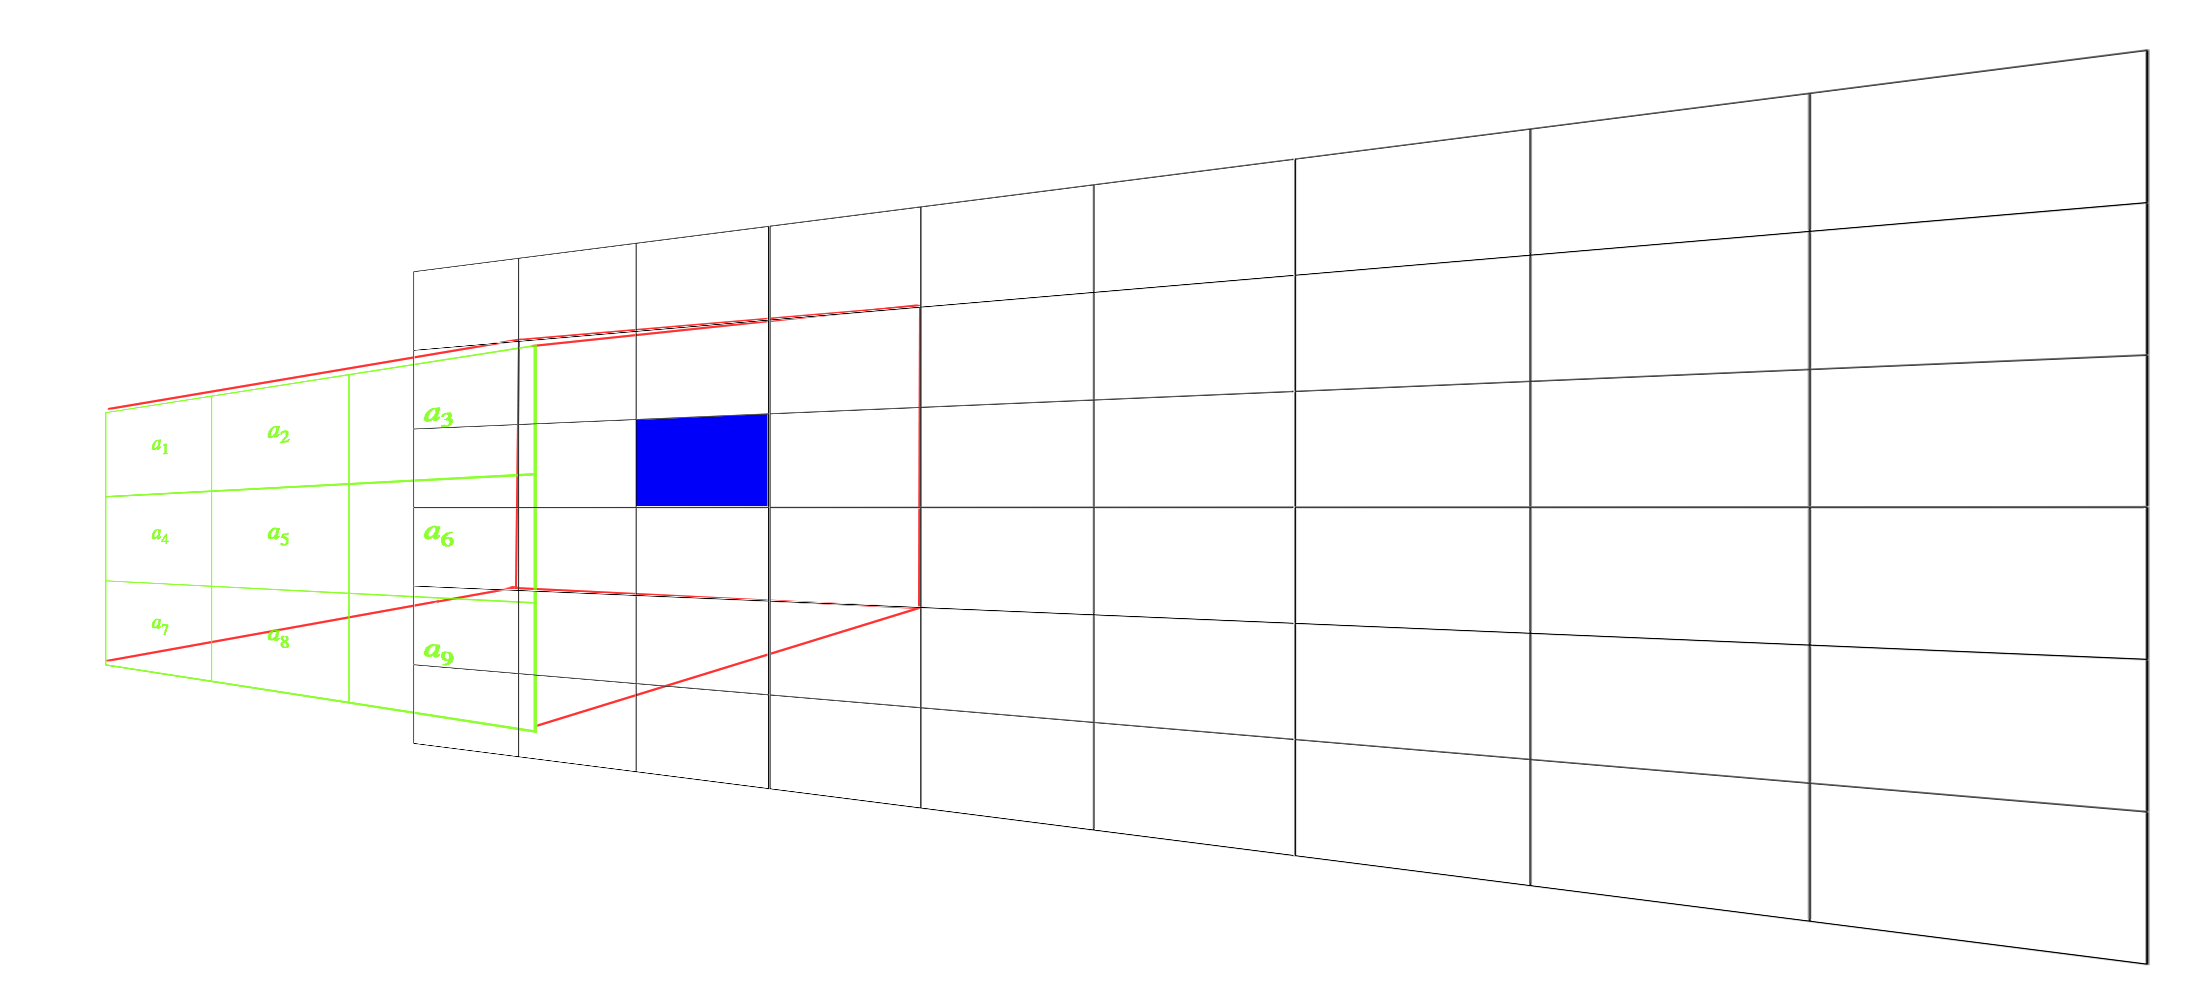
\includegraphics[scale=0.15]{Pictures/illustrazione convoluzione.png}
    \caption{Griglia dell'immagine in nero, maschera in verde, pixel in esame in blu}
    \label{fig:my_label}
\end{figure}
Per ogni pixel ne viene ricalcolato il valore come segue
\begin{figure}
    \centering
    %\begin{tabular}{|c|c|c|}
    \begin{tabular}{|p{1.6cm}|p{1.6cm}|p{1.6cm}|}
        \hline
        \makebox[1.6cm][c]{
        \rule[-8mm]{0cm}{1.6cm}
        $p_{i-1,j+1}$} & 
        \makebox[1.6cm][c]{
        $p_{i,j+1}$} & 
        \makebox[1.6cm][c]{
        $p_{i+1,j+1}$} \\
        \hline
        \makebox[1.6cm][c]{
        \rule[-8mm]{0cm}{1.6cm}
        $p_{i-1,j}$} & 
        \makebox[1.6cm][c]{
        $p_{i,j}$} & 
        \makebox[1.6cm][c]{
        $p_{i+1,j}$} \\
        \hline
        \makebox[1.6cm][c]{
        \rule[-8mm]{0cm}{1.6cm}
        $p_{i-1,j-1}$} & 
        \makebox[1.6cm][c]{
        $p_{i,j-1}$} & 
        \makebox[1.6cm][c]{
        $p_{i+1,j-1}$} \\
        \hline
    \end{tabular}
    \hspace{1em}
    \huge{*}
    \normalsize
    \hspace{1em}
    \begin{tabular}{|p{1.6cm}|p{1.6cm}|p{1.6cm}|}
        \hline
        \makebox[1.6cm][c]{
        \rule[-8mm]{0cm}{1.6cm}
        $a_1$} & 
        \makebox[1.6cm][c]{
        $a_2$} & 
        \makebox[1.6cm][c]{
        $a_3$} \\
        \hline
        \makebox[1.6cm][c]{
        \rule[-8mm]{0cm}{1.6cm}
        $a_4$} & 
        \makebox[1.6cm][c]{
        $a_5$} & 
        \makebox[1.6cm][c]{
        $a_6$} \\
        \hline
        \makebox[1.6cm][c]{
        \rule[-8mm]{0cm}{1.6cm}
        $a_7$} & 
        \makebox[1.6cm][c]{
        $a_8$} & 
        \makebox[1.6cm][c]{
        $a_9$} \\
        \hline
    \end{tabular}
    \small{
    $$
    u(p_{i,j})*F=a_1p_{i-1,j+1} + a_2p_{i,j+1} + a_3p_{i+1,j+1} + a_4p_{i-1,j} + a_5p_{i,j} + a_6p_{i+1,j} + a_7p_{i-1,j-1} + a_8p_{i,j-1} + a_9p_{i+1,j-1}.
    $$
    }\\
\caption{Intorno di un punto, maschera di convoluzione e soluzione analitica}
\label{fig:my_label}
\end{figure}

\vspace{-1em}

Ma allora una convoluzione con $a=$
    \begin{tabular}{|p{0.4cm}|p{0.4cm}|p{0.4cm}|}
        \hline
        \makebox[0.4cm][c]{
        \rule[-2mm]{0cm}{0.6cm}
        $0$} & 
        \makebox[0.4cm][c]{
        $1$} & 
        \makebox[0.4cm][c]{
        $0$} \\
        \hline
        \makebox[0.4cm][c]{
        \rule[-2mm]{0cm}{0.6cm}
        $0$} & 
        \makebox[0.4cm][c]{
        $-1$} & 
        \makebox[0.4cm][c]{
        $0$} \\
        \hline
        \makebox[0.4cm][c]{
        \rule[-2mm]{0cm}{0.6cm}
        $0$} & 
        \makebox[0.4cm][c]{
        $0$} & 
        \makebox[0.4cm][c]{
        $0$} \\
        \hline
    \end{tabular}
\vspace{0.5em}
vuol dire fare la derivata prima approssimata alle differenze finite lungo y, in particolare verso l'alto, infatti facendo il conto di cui sopra si ottiene $u(p_{i,j})*F=p_{i,j+1}-p_{i,j}$ che è esattamente quanto trovato analizzando il metodo alle differenze finite
si può operare analogamente in tutte e 4 le direzioni.\\
\vspace{1em}
Per facilitare la successiva implementazione del filtro, si è scritta una funzione MATLAB che operi in tal senso.

\begin{lstlisting}[language=MATLAB]
function B=convoluzione(A,k);

[r c] = size(A);            %Memorizzo le dimensioni dell'immagine
[m n] = size(k);            %Memorizzo le dimensioni della maschera
h = rot90(k, 2);

%Definisco una cornice per gestire gli effetti di bordo
center = floor((size(h)+1)/2);                  
left = center(2) - 1;
right = n - center(2);
top = center(1) - 1;
bottom = m - center(1);

%Preparo un "piano di lavoro"
Rep = zeros(r + top + bottom, c + left + right);
for x = 1 + top : r + top
    for y = 1 + left : c + left
        Rep(x,y) = A(x - top, y - left);
    end
end

%Opero la convoluzione
B = zeros(r , c);
for x = 1 : r
    for y = 1 : c
        for i = 1 : m
            for j = 1 : n
                q = x - 1;
                w = y -1;
                B(x, y) = B(x, y) + (Rep(i + q, j + w) * h(i, j));
            end
        end
    end
end

\end{lstlisting}
Notare che \texttt{Rep} ha dimensioni maggiori rispetto all'immagine questo perchè dobbiamo gestire anche i pixel sui bordi del riquadro dell'immagine. Volendo fare un esempio, si consideri il pixel in posizione (1,1), ossia l'angolo in alto a sinistra, allora i coeff $a_1$, $a_2$, $a_3$, $a_4$ e $a_7$, non avranno nessun corrispettivo da moltiplicare, costruiamo quindi una cornice nera (cioè pixel di valore nullo) per ovviare a questo problema. Ovviamente se la maschera è grande, questo porterà a dei visibili errori di bordo, il che è esattamente il motivo per cui si usano solitamente maschere di dimensioni molto piccole.




\newpage
\subsection{Rilevamento dei bordi}
Il metodo Perona-Malik serve ad eliminare il rumore, preservando i bordi. Per essere in grado di preservarli però dobbiamo prima essere in grado di riconoscerli. Il metodo prevede l'introduzione del termine $K(\Delta(u))$ che dipende quindi dal laplaciano dell'immagine che si intende filtrare. Cerchiamo di capire il perché di questa scelta.\\
\vspace{1em}
Operando una derivata in una data direzione, per il significato in sè di derivata, questa assume valori più elevati quando la variazione è elevata, e assume valori nulli quando non c'è variazione in quella direzione. Per questo motivo, applicata ad un' immagine, ne rileviamo i bordi.\\
Presa una tinta unita la derivata sarà quindi nulla in ogni suo punto (è intuitivo: se un'immagine è una funzione che, date due coordinate restituisce un colore, allora una tinta unita è una funzione costante ed in quanto tale ha derivata nulla).\\
Operando una derivata seconda in una data direzione, per il significato in sè di derivata seconda, questa assume valori più elevati quando la concavità è più stretta, e assume valori pressocchè nulli quando non ci sono concavità (si può pensare alle concavità come a dei picchi o dei ventri, su di una immagine vuol dire chiazze di colore diverso).\\
Presa una sfumatura di colore che varia in maniera lineare, la derivata seconda sarà nulla in ogni suo punto, la derivata prima sarà invece costante.\\x
\vspace{1em}
Per verificare la validità di questi concetti teorici si è implementato un semplice script MATLAB che, presa un'immagine, opera il calcolo delle derivate e stampa a video le sole derivate sotto forma di immagine. Ne risulterà quindi un'immagine in bianco e nero con pixel quanto più chiari quanto più e alto il valore della derivata. Saranno mostrate come immagini diverse le derivate parziali, il gradiente ed il laplaciano dell'immagine data in input, così da poterli confrontare ed evidenziarne le differenze. Ci aspettiamo che le immagini risultanti corrispondano con i bordi dell'immagine originale.\\
Saranno mostrati i risultati prodotti da tale script dandogli in input immagini di diverso tipo, saranno poi commentati con osservazioni e considerazioni di vario tipo.
\newpage
Si riporta lo script MATLAB appena citato.
\vspace{1em}
\begin{lstlisting}[language=MATLAB]
%---Operazioni preliminari
Im=imread("nome_immagine.png");	%Apro l'immmagine

[ny, nx, ~]=size(Im)        %Memorizzo le dimensioni dell'immagine
u=double(Im);               %Copia dell'immagine originale su cui lavorare
h=80;                       %Definisco un parametro che usero' per                               enfatizzare i bordi in fase di stampa 


%---Calcolo tutte le derivate
u_x =  u(:,[1 1:nx-1],:) - u;                       %derivata                                                            prima lungo x
u_xx = u(:,[2:nx nx],:) - 2*u + u(:,[1 1:nx-1],:);  %derivata                                                            seconda lungo x
u_y =  u([1 1:ny-1],:,:) - u;                       %derivata                                                            prima lungo y
u_yy = u([2:ny ny],:,:) - 2*u + u([1 1:ny-1],:,:);  %derivata                                                            seconda lungo y
u_xy = u_x([1 1:ny-1],:,:) - u_x;                   %derivata                                                            seconda mista
   
%---Stampo i risultati
figure()
subplot(2,3,2),text(0.3,0,nome,'FontSize',20); axis off
subplot(2,3,4), imshow(Im)
title('Immagine originale')
subplot(2,3,5), imshow(uint8(h*abs(u_x)))
title('h*u_x')
subplot(2,3,6), imshow(uint8(h*abs(u_y)))
title('h*u_y')

figure()
subplot(2,3,2),text(0.3,0,nome,'FontSize',20); axis off
subplot(2,3,4), imshow(Im)
title('Immagine originale')
subplot(2,3,5), imshow(uint8(h*abs(u_x + u_y)))
title('h*(u_x + u_y)')
subplot(2,3,6), imshow(uint8(h*abs(u_xx + u_yy)))
title('h*(u_{xx} + u_{yy})')
\end{lstlisting}

\vspace{1em}
Eseguiamo adesso questo script che ci permetterà di osservare, fornendogli in input diverse immagini molto semplici, se abbiamo ottenuto i risultati attesi.\\
%\vspace{1em}
\newpage
\subsubsection{Esempio 1 - Tinta unita}
\begin{figure}[htb]
\centering
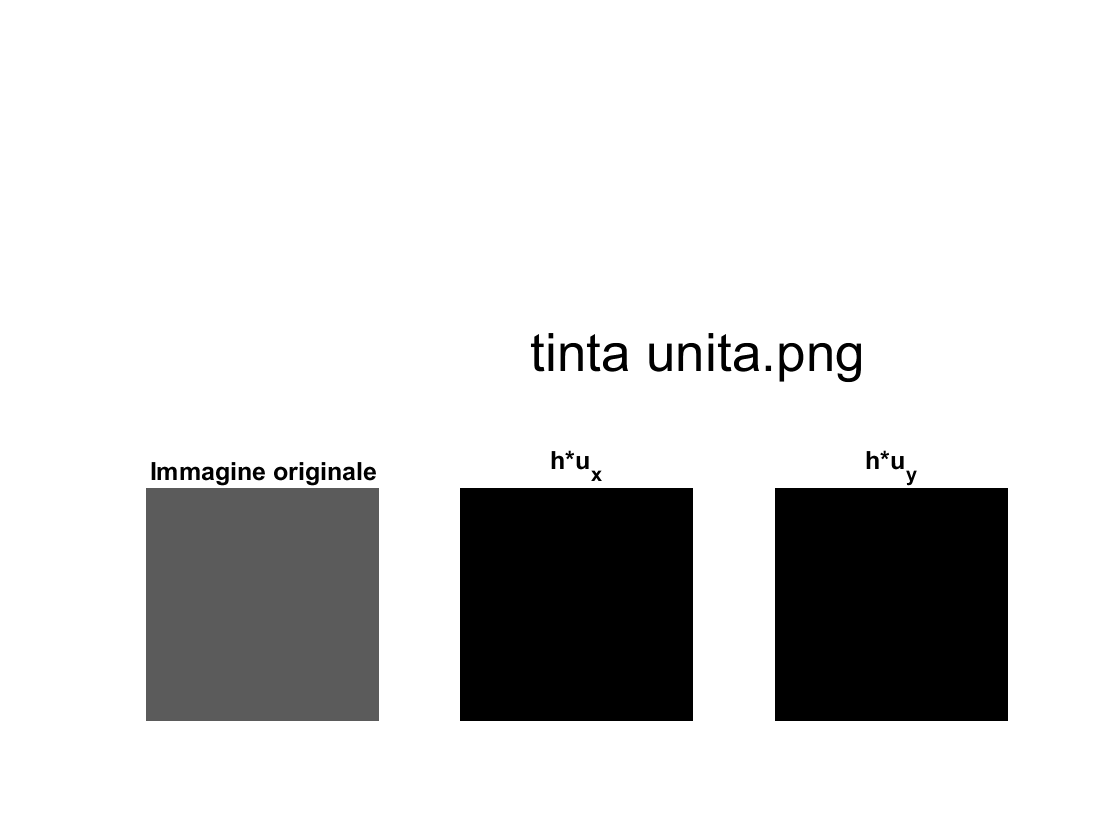
\includegraphics[scale=0.4, trim = 0 2cm 0 11.5cm, clip]{Pictures/Risultati/tinta unita bianco e nero derivate parziali.png}
%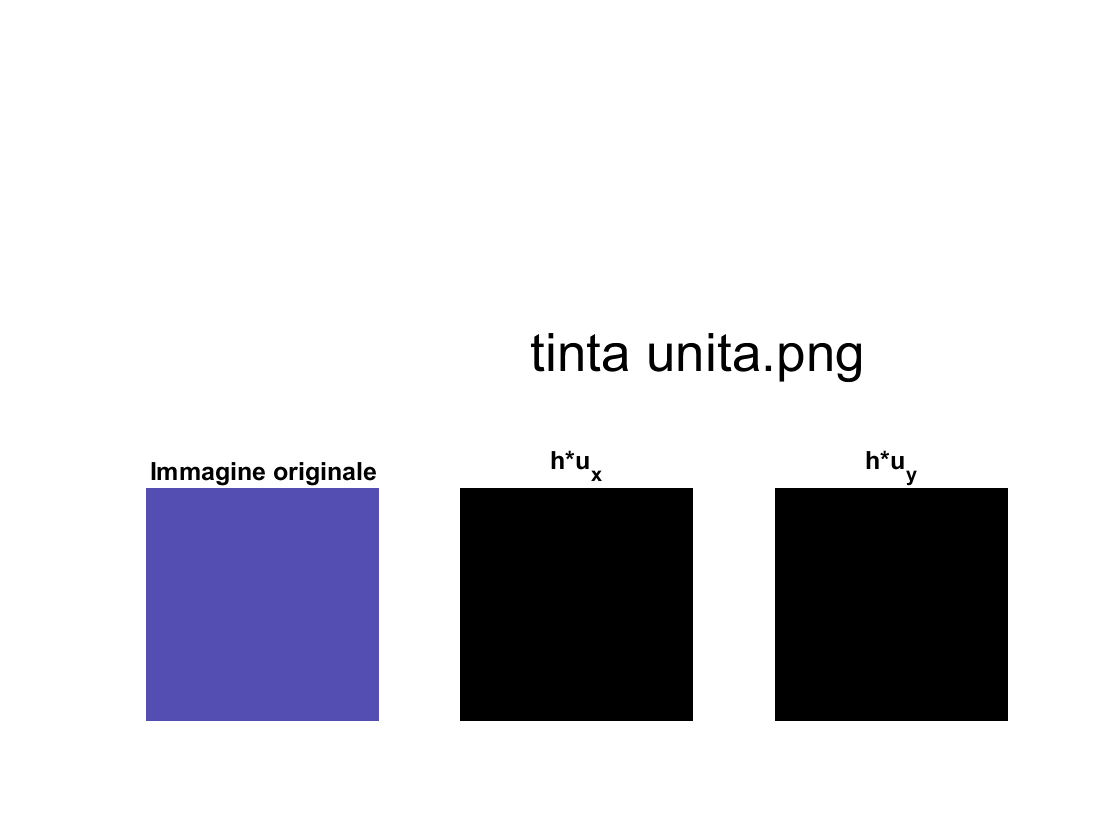
\includegraphics[scale=0.4, trim = 0 0 0 10.5cm, clip]{Pictures/Risultati/tinta unita derivate parziali.png}
\caption{Derivate parziali di una tinta unita.}\label{fig:figura}
\end{figure}

Si può vedere come con un'immagine a tinta unita le derivate sono nulle, quindi lo saranno anche gradiente e laplaciano.\\

\subsubsection{Esempio 2 - Sfumatura lungo l'asse x}
\begin{figure}[htb] 
\centering
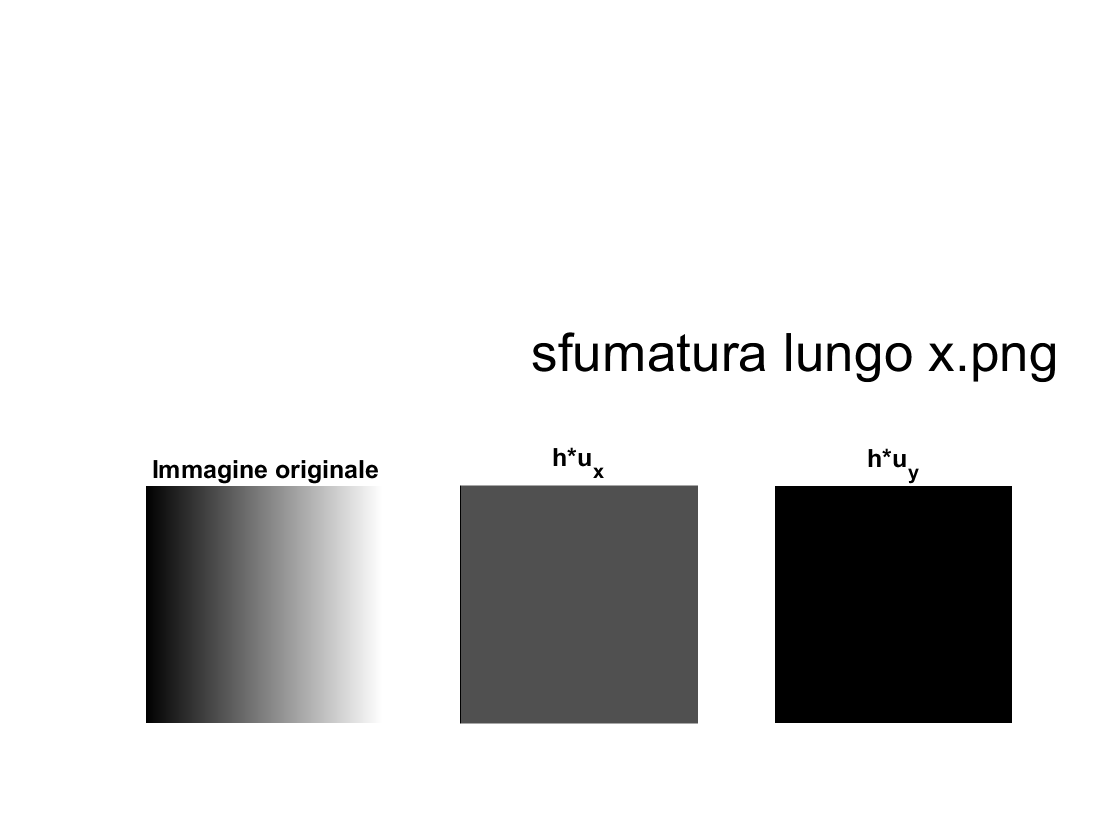
\includegraphics[scale=0.4, trim = 0 2cm 0 11.5cm, clip]{Pictures/Risultati/sfumatura lungo x bianco e nero derivate parziali.png}
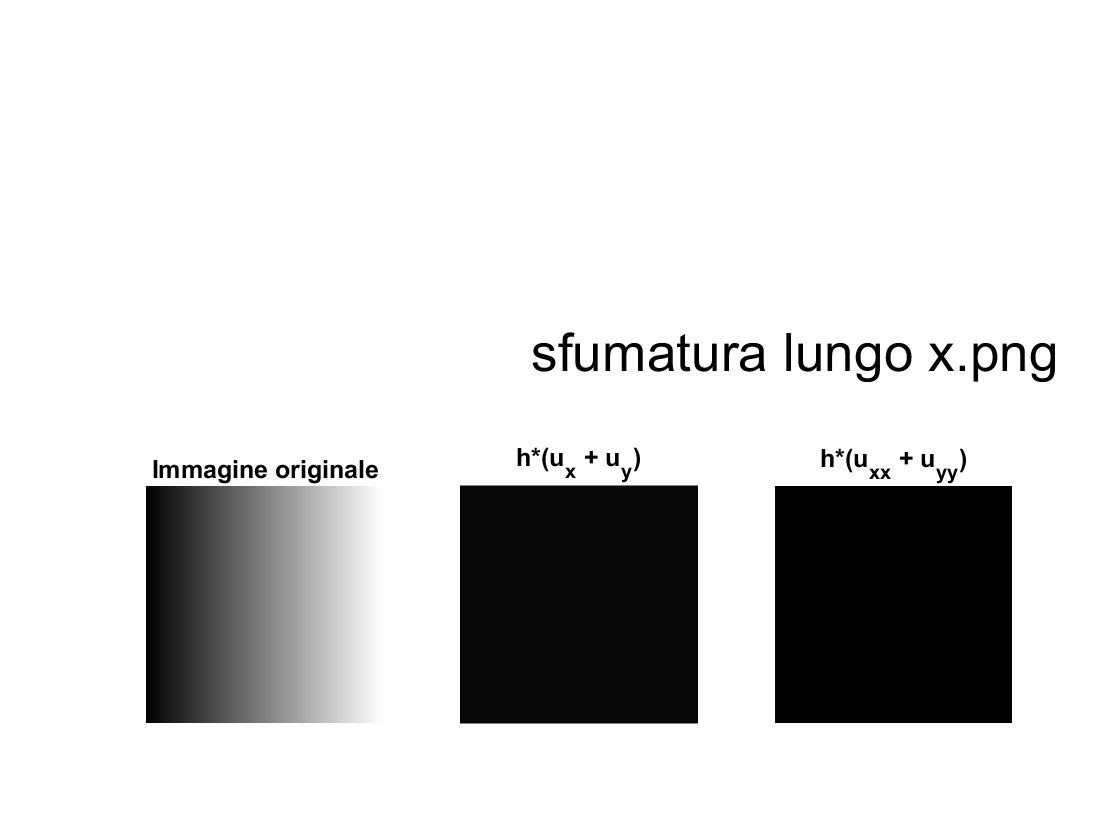
\includegraphics[scale=0.4, trim = 0 2cm 0 11.5cm, clip]{Pictures/Risultati/sfumatura lungo x bianco e nero gradiente e laplaciano.png}
\caption{Derivate parziali, gradiente e laplaciano di una sfumatura orizzontale.}\label{fig:figura}
\end{figure}

Guardando invece ad una immagine che presenta una sfumatura lineare lungo l'asse x, la derivata lungo x assume un valore costante mentre la derivata lungo y è nulla, proprio perchè lungo y non c'è variazione mentre lungo x c'è una variazione costante.\\
Ovviamente, date queste premesse, il gradiente sarà costante uguale ad $u_x$ (siccome $u_y=0$) e quindi il laplaciano sarà nullo.
Il fatto che in entrambi questi esempi il laplaciano sia nullo è un buon segno, lo useremo per rilevare i bordi ed in queste immagini non ve ne sono, quindi è giusto che il laplaciano sia nullo.\\

\newpage
\subsubsection{Esempio 3 - Parziale sfumatura lungo la diagonale}
\begin{figure}   
\centering
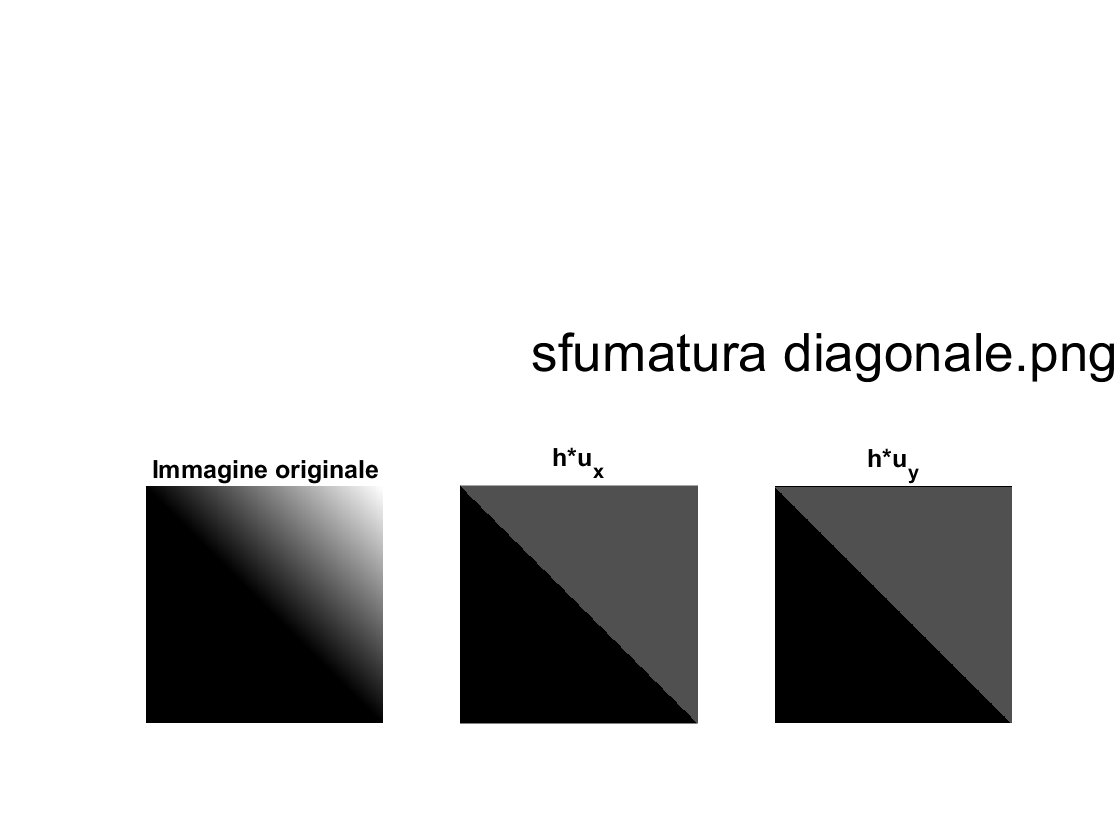
\includegraphics[scale=0.4, trim = 0 0 0 10.5cm, clip]{Pictures/Risultati/sfumatura diagonale bianco e nero derivate parziali.png}
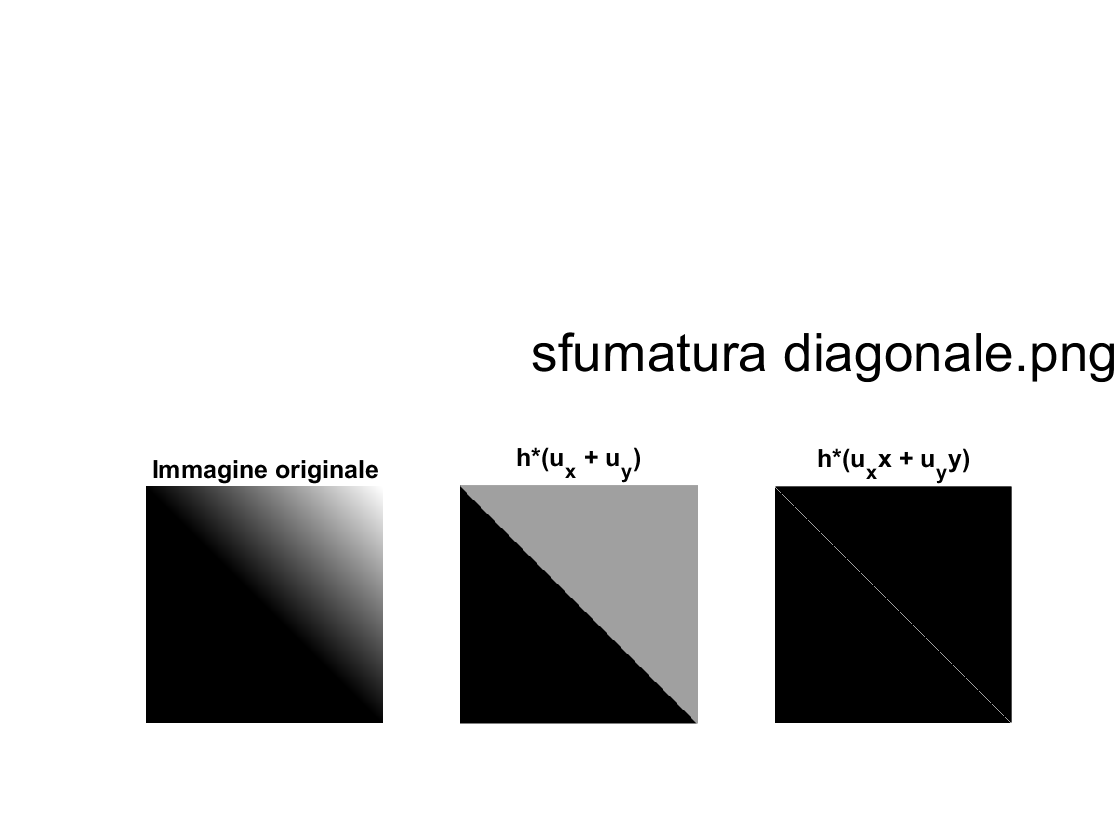
\includegraphics[scale=0.4, trim = 0 0 0 10.5cm, clip]{Pictures/Risultati/sfumatura diagonale bianco e nero gradiente e laplaciano.png}
\caption{Derivate parziali, gradiente e laplaciano di una parziale sfumatura diagonale.}\label{fig:figura}
\end{figure}

Presa una sfumatura diagonale, ma solo su metà immagine vediamo dei risultati interessanti: entrambe le derivate parziali sono nulle nelle regioni in cui non c'è sfumatura, esattamente come nel caso della tinta unita, ed entrambe sono costanti dove c'è sfumatura (che ricordiamo essere lineare).\\
Tutto ciò riconferma quanto visto dai punti precedenti, volgendo quindi uno sguardo al gradiente ed al laplaciano si può notare che mentre il gradiente ha un aspetto molto simile alle due derivate parziali, sommando i loro valori è semplicemente più luminoso, per quanto riguarda il laplaciano la storia cambia. Le derivate seconde sono indicatrici della variazione delle derivate prime, cioè della variazione della variazione del valore della funzione, ma l'unica variazione che hanno le derivate prime è lungo la diagonale.
Abbiamo così individuato il nostro primo bordo, cioè la diagonale che divide di fatto due regioni, una in cui il colore è costante ed una in cui sfuma.\\

\vspace{1em}
Si riportano ancora due varianti di un'ultima immagine esempio, provando ad introdurre una semplice figura.\\

\newpage
\subsubsection{Esempio 4 - Rettangolo bianco su sfondo nero}
\begin{figure}[htb] 
\centering
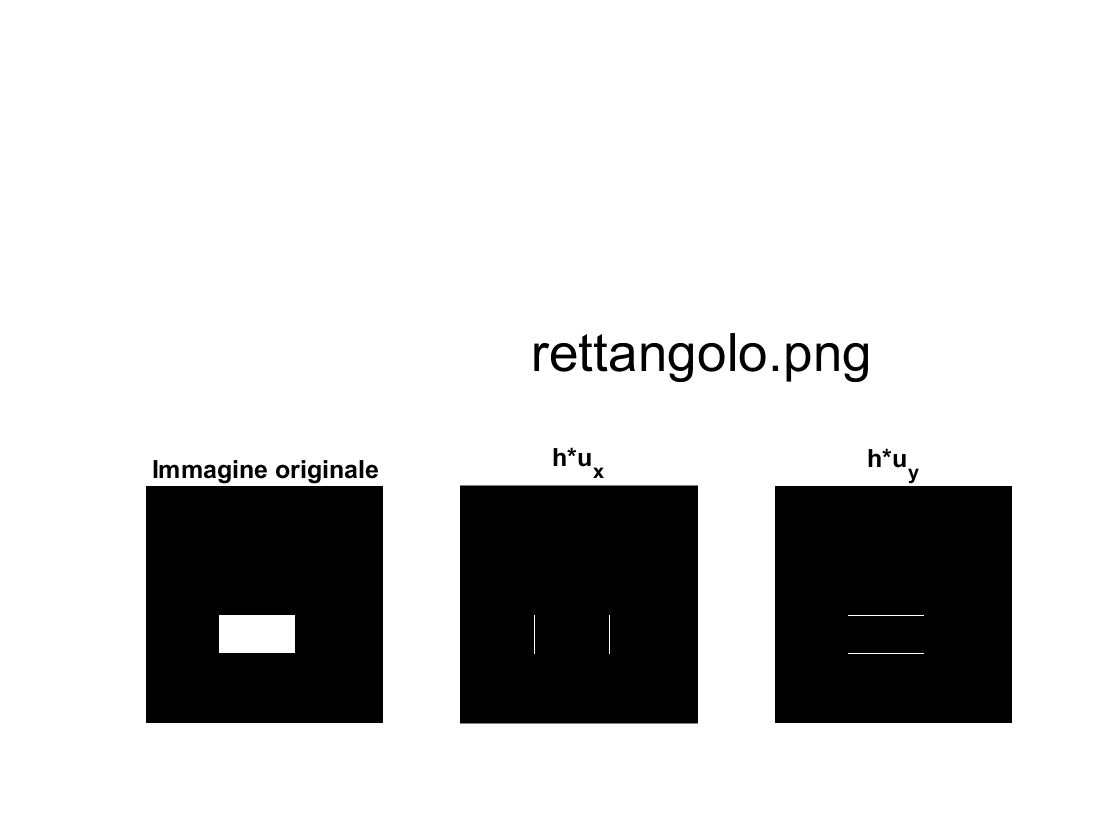
\includegraphics[scale=0.4, trim = 0 0 0 10.5cm, clip]{Pictures/Risultati/rettangolo bianco e nero derivate parziali.png}
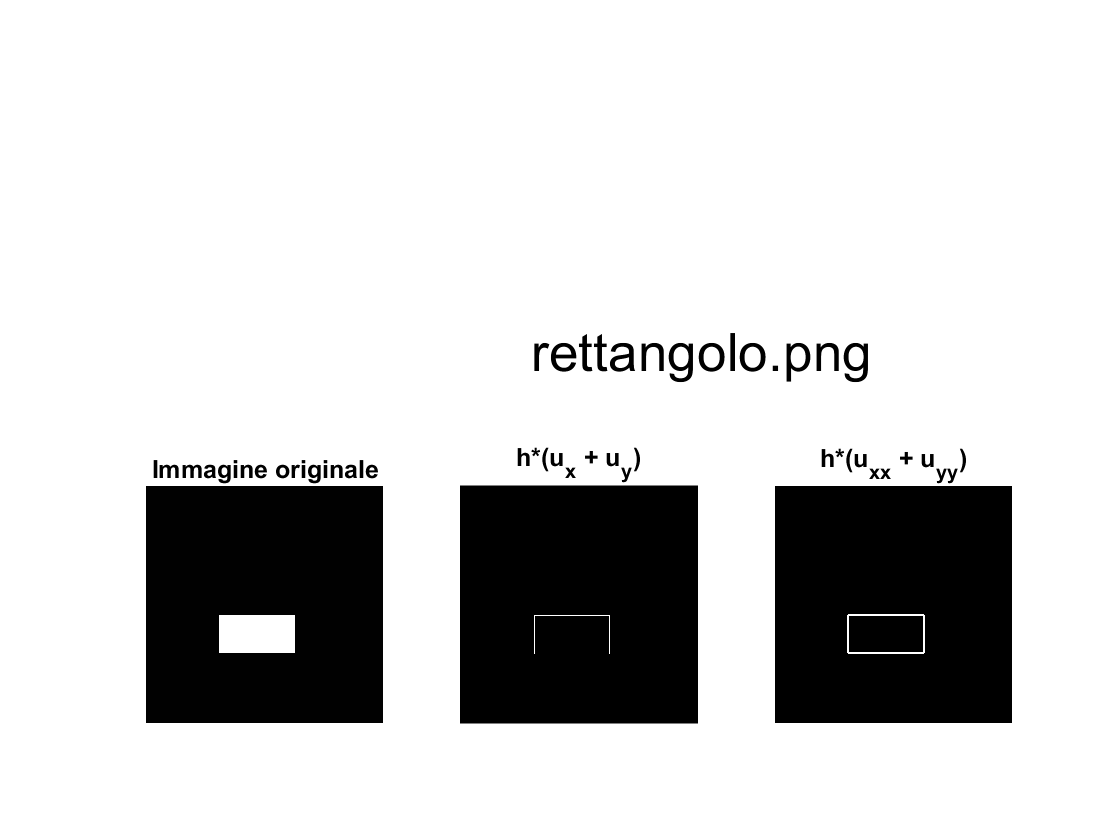
\includegraphics[scale=0.4, trim = 0 0 0 10.5cm, clip]{Pictures/Risultati/rettangolo bianco e nero gradiente e laplaciano.png}
\caption{Derivate parziali, gradiente e laplaciano di una figura semplice.}\label{fig:figura}
\end{figure}

Importando un rettangolo bianco su di uno sfondo nero, come confermato anche dalla prima sfumatura, la derivata lungo x rileva i bordi verticali, quella lungo y i bordi orizzontali, dalla loro somma (quindi dal gradiente) otteniamo già il bordo del rettangolo.
Il bordo così ottenuto è un bordo che idealmente rimarrà inalterato a prescindere dall'ordine della derivata, in particolare quindi anche per derivate seconde, quindi il laplaciano continua a soddisfare la richiesta di determinare i bordi. \\
Come detto: \textit{"Il bordo così ottenuto è un bordo che idealmente rimarrà inalterato a prescindere dall'ordine della derivata"} è interessante capire perchè. Presa una striscia di pixel, cioè uno strato dell'immagine (la si può immaginare quindi come una funzione $u_y:\mathbb{R} \longrightarrow \mathbb{R}$), risulterà essa raffigurare una funzione porta!\\
La funzione porta non è derivabile in senso classico, ripensando alla definizione di derivata avremmo un valore di +infinito prima e -infinito poi. La sua derivata sarà quindi una coppia di delta di Dirac.\\

\vspace{1em}
Proviamo in fine ad introdurre del rumore in quest'ultima immagine e osserviamo cosa accade.

\newpage
\subsubsection{Esempio 5 - Rettangolo bianco su sfondo dietro con rumore}
\begin{figure}   
\centering
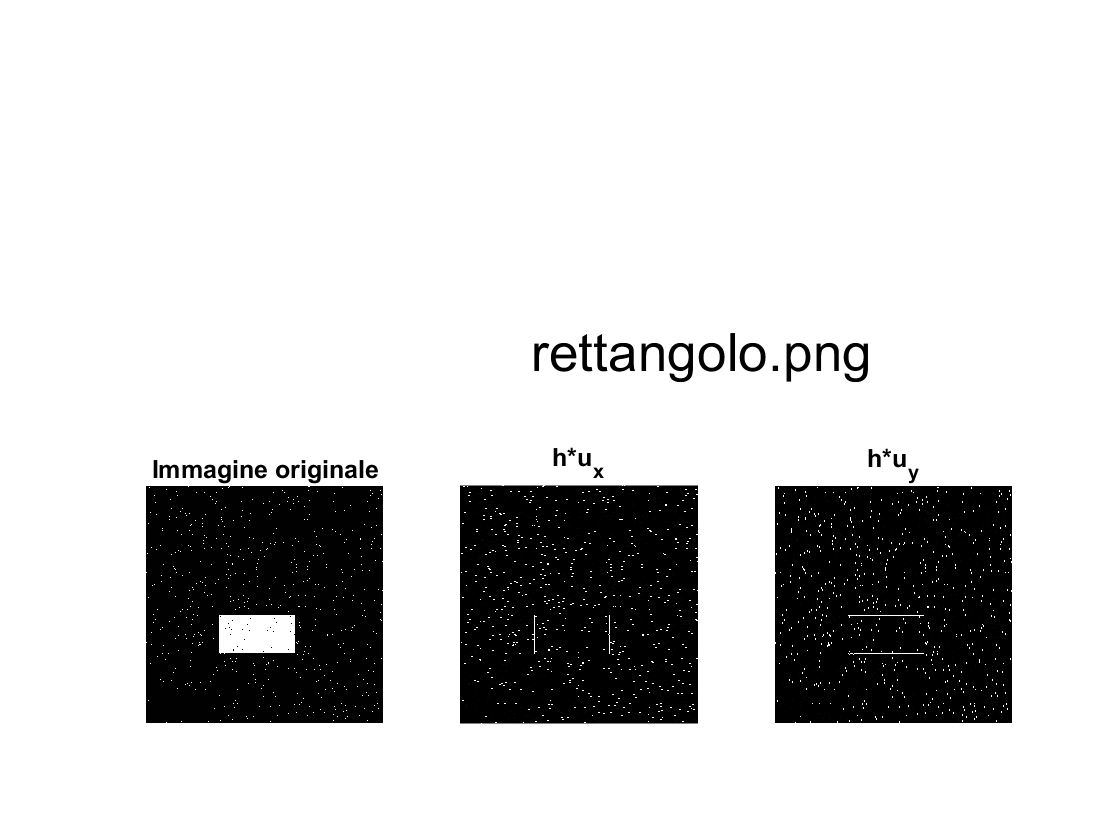
\includegraphics[scale=0.4, trim = 0 0 0 10.5cm, clip]{Pictures/Risultati/rettangolo bianco e nero derivate parziali con rumore.png}
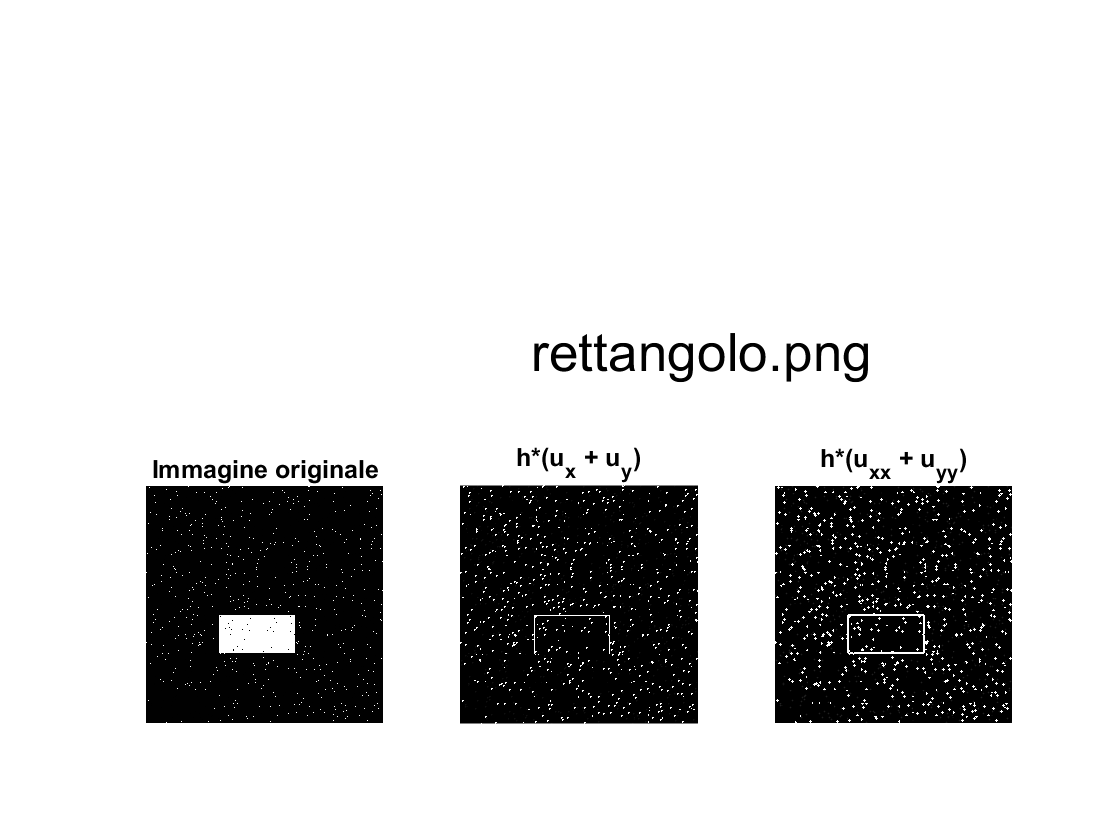
\includegraphics[scale=0.4, trim = 0 0 0 10.5cm, clip]{Pictures/Risultati/rettangolo bianco e nero gradiente e laplaciano con rumore.png}
\caption{Derivate parziali, gradiente e laplaciano di una figura semplice con rumore.}\label{fig:figura}
\end{figure}

Si può fare una considerazione: quando si trova un elemento di disurbo, come un puntino o una chiazza di colore, questo risulterà essere una forte variazione di colore improvvisa ed in quanto tale la derivata calcolata in un intorno di quel punto sarà, in valore assoluto, molto alta.
Questo vuol dire che il gradiente ne rileverà i bordi e il metodo Perona-Malik non lo toccherà, questa cosa non va bene: è un elemento di disturbo e va quindi eliminato.\\ 
Una possibile soluzione a questo problema verrà illustrata in seguito.\newpage


\newpage 
\subsection{Problema dei \textit{"bordi"} d'interferenza}
%\subsubsection{Considerazioni sui bordi}
%\subsubsection{Miglioramento dei bordi}
Come evidenziato con l'ultima immagine di prova nella sezione dedicata al rilevamento dei bordi, anche gli elementi di disturbo ne hanno e vengono quindi rilevati. Questo è un problema perché il metodo Perona-Malik tenderà a preservarli.\\
Per ovviare a questo problema operiamo su di una copia dell'immagine una diffusione come quella operata dall'equazione del calore vista in precedenza, così facendo in questa copia, i bordi dell'immagine risulteranno rovinati, ma non scomparsi! Gli elementi di disturbo saranno invece eliminati.\\
Moltiplicando i due gradienti così trovati si può osservare che: in corrispondenza degli elementi di disturbo il secondo gradiente sarà nullo ed il prodotto sarà dunque anch'esso nullo, vicino ai bordi il secondo gradiente non è nullo, ma il primo sì! Quindi il prodotto sarà ancora nullo, in corrispondenza degli effettivi bordi entrambi i gradienti saranno non nulli e quindi neanche il loro prodotto lo sarà. Questo vuol dire che:\\
\begin{itemize}
    \item gli elementi di disturbo sono stati eliminati
    \item l'effetto distruttivo sui bordi non viene riportato
    \item gli effettivi bordi dell'immagine vengono preservati
\end{itemize}
I bordi sono quindi calcolati in maniera efficiente.\\
\vspace{0em}
\subsubsection{La funzione di controllo}
\`E doveroso fare ancora una considerazione. Serve applicare ancora una trasformazione ai nostri bordi in modo da risultare ancor più efficienti ai nostri scopi, ossia una funzione di controllo. Cerchiamo una funzione decrescente tale che $k(0)=1$ e $\lim_{s\to\infty}k(s)=0$. Daremo in input a tale funzione il valore del gradiente calcolato in ogni pixel, otterremo così una mappatura che ci dice per ogni pixel in che misura operare la diffusione. Calato nel caso di studio, $k(0)=1$ vuol dire che dove non c'è bordo opera l'equazione del calore mentre $\lim_{|\nabla(u)|^2\to\infty}k(|\nabla(u)|^2)=0$ vuol dire che tanto più i bordi sono accentuati, tanto più l'equazione del calore non deve operare.
Facciamo questo banalmente perché considerando semplicemente i bordi, avremmo l'effetto opposto! Infatti dove non ci sono bordi $\nabla(u)=0$ e quindi non ci sarebbe diffusione, dove ci sono bordi molto marcati $\nabla(u)\to\infty$ quindi la diffusione verrebbe adoperata addirittura più del normale!
Non a caso una delle scelte più semplici, anche se non delle più classiche nè efficienti è $k=\frac{1}{1+|\nabla(u)|^2/c}$ dove c è un fattore di controllo.
Scelte decisamente più classiche ed impiegate sono:
\begin{itemize}
    \item $k=e^{-\frac{|\nabla(u)|^2}{c}}$ che preserva maggiromente i bordi ad altro constrasto e meno quelli a basso contrasto
    \item $k=\frac{1}{\sqrt{1+(|\nabla(u)|^2/c)}}$ che preserva maggiormente regioni grandi piuttosto che quelle piccole
\end{itemize} 
Come visto nella sezione 2.2.1 $div(k\nabla(u))=\frac{1}{2}(k_N\nabla_N + k_S\nabla_S k_W\nabla_W + k_E\nabla_E)$ calcoliamo quindi i vettori $k_N$, $k_S$, $k_W$ e $k_E$ dando in input alla funzione di controllo scelta i vettori $\nabla_N$, $\nabla_S$, $\nabla_W$ e $\nabla_E$ rispettivamente.

\newpage
\subsection{Implementazione}
Nel corso della trattazione sono stati forniti tutti gli elementi che portano alla formazione di questo script. Ci si limiterà quindi a dei richiami e a delle precisazioni di tipo tecnico.\\
\vspace{1em}
Prima di iniziare il filtraggio ci sono alcune operazioni preliminari da fare. In primo luogo occorrerà, ovviamente, caricare l'immagine che si intende filtrare. Successivamente l'immagine viene convertita in bianco e nero e viene aggiunto del rumore.\\
\begin{lstlisting}[language=MATLAB, name=listato]
img=imread('nome_file.png');            %Apertura dell'immmagine
img=rgb2gray(img);                      %Trasformazione in bianco e nero
im = imnoise(im,'salt & pepper',0.02);  %Aggiunta del rumore
\end{lstlisting}
\`E importante precisare che quest'ultima operazione, in un caso reale, non ha senso di esistere ma è messa lì per il puro scopo di simulare il problema che intendiamo risolvere.
\begin{lstlisting}[language=MATLAB, name=listato]
% conversione in double per il calcolo.
im = double(im);
\end{lstlisting}
Di norma codifichiamo le immagini come uint8 (interi senza segno da 0 a 255), tuttavia mantenere questa formattazione durante il calcolo potrebbe portare ad errori di approssimazione numerica assolutamente non trascurabili. Consideriamo quindi matrici a valori reali, approssimate dalla macchina a numeri macchina a doppia precisione. 
\begin{lstlisting}[language=MATLAB, name=listato]
% Condizioni iniziali della PDE.
diff_im = im;

num_iter=20;                            %numero di iterazioni
delta_t=0.1;                            %costante d'integrazione
c=60;                                   %coefficiente di controllo del                                       gradiente

sigma=1;                                %costante di controllo della                                         diffusione uniforme

\end{lstlisting}
Occorre settare alcuni parametri per il calcolo: 
\begin{itemize}
    \item Numero di iterazioni per il metodo di Eulero: maggiore è il valore di questo parametro e più volte verrà applicato il metodo
    \item Costante d'integrazione: maggiore è il valore di questo parametro e maggiore sarà l'intensità con cui viene applicato il metodo\\
    \vspace{0.25em}
    \textit{N.B. Sia aumentando il primo parametro sia il secondo ciò che otterremo sarà un'immagine filtrata maggiormente. La differenza è che aumentando la costante di integrazione applicheremo il metodo con maggior intensità ad ogni passo; invece aumentando il numero di iterazioni applicheremo il metodo un numero maggiore di volte. 
    Ad ogni iterazione tutti i calcoli andranno rifatti, ciò vuol dire che aumentando il numero di iterazioni e riducendo la costante di integrazione, avremo un'immagine filtrata più finemente a discapito di un grosso aumento di costo computazionale}
    \item Coefficiente di controllo del gradiente: permette di far risaltare di più (se c<1) o di meno (se c>1) i bordi
    \item costante di controllo diffusione uniforme: il calcolo del vettore c utilizzato per modificare l'equazione del calore avviene tramite gradiente. Come già analizzato nella sezione 5.3, conviene fare questo calcolo su una versione sfocata dell'immagine, per fare ciò applichiamo l'equazione del calore. Modificarne questo cofficiente significa modificare l'intensità con cui viene applicata. Un valore più alto sfoca di più e porta ad eliminare più rapidamente il rumore a discapito della definizione dei bordi.
\end{itemize}
Settati i parametri inizia il calcolo effettivo
\begin{lstlisting}[language=MATLAB, name=listato]

% Maschera di convoluzione
hN = [0 1 0; 0 -1 0; 0 0 0];
hS = [0 0 0; 0 -1 0; 0 1 0];
hE = [0 0 0; 0 -1 1; 0 0 0];
hW = [0 0 0; 1 -1 0; 0 0 0];


for t = 1:num_iter
   
    % Calcolo alle differenze finite nelle 4 direzioni
    nablaN = convoluzione(diff_im,hN);
    nablaS = convoluzione(diff_im,hS);   
    nablaW = convoluzione(diff_im,hW);
    nablaE = convoluzione(diff_im,hE);
    
    diff_blur = f_eq_del_calore(diff_im,delta_t,num_iter,sigma);
    nablaN_blur = convoluzione(diff_blur,hN);
    nablaS_blur = convoluzione(diff_blur,hS);   
    nablaW_blur = convoluzione(diff_blur,hW);
    nablaE_blur = convoluzione(diff_blur,hE);


    kN = exp(-(nablaN_blur/c).^2);
    kS = exp(-(nablaS_blur/c).^2);
    kW = exp(-(nablaW_blur/c).^2);
    kE = exp(-(nablaE_blur/c).^2);
\end{lstlisting}
Calcolati tutti i fattori possiamo in fine applicare il metodo utilizzando la formula trovata nella sezione 5.1
\begin{lstlisting}[language=MATLAB, name=listato]
    % Soluzione discreta della PDE.
    diff_im = diff_im + delta_t*(kN.*nablaN + kS.*nablaS + kW.*nablaW + kE.*nablaE );
          
\end{lstlisting}
Concludiamo stampando l'immagine rumorosa e quella filtrata per poter apprezzare gli effetti sortiti
\begin{lstlisting}[language=MATLAB, name=listato]
    % Stampa di controllo
    fprintf('\rIteration %d\n',t);
end
% Stampa dei risultati
figure('Name','Original picture');      %Stampa dell'immagine rumorosa
imshow(im);
figure('Name','Perona Malik');          %Stampa dell'immagine filtrata
imshow(uint8(diff_im));

\end{lstlisting}

\newpage
\chapter{Esempi di utilizzo}
\section{Esempi di utilizzo}
Ultimata l'implementazione del metodo è bene spendere del tempo per testarne l'efficacia ed osservare come i vari parametri influenzano i risultati ottenuti.\\
Richiamiamo il significato teorico dei vari parametri:
\begin{itemize}
    \item num\_iter (numero di iterazioni per il metodo di Eulero): maggiore è il valore di questo parametro e più volte verrà applicato il metodo
    \item delta\_t (costante d'integrazione): maggiore è il valore di questo parametro e maggiore sarà l'intensità con cui viene applicato il metodo\\
    \item c (coefficiente di controllo del gradiente): permette di far risaltare di più (se c<1) o di meno (se c>1) i bordi
    \item sigma (costante di controllo diffusione uniforme): il calcolo del vettore c utilizzato per modificare l'equazione del calore avviene tramite gradiente. Come già analizzato nella sezione 5.3, conviene fare questo calcolo su una versione sfocata dell'immagine, per fare ciò applichiamo l'equazione del calore. Modificarne questo coefficiente significa modificare l'intensità con cui viene applicata. Un valore più alto sfoca di più e porta ad eliminare più rapidamente il rumore a discapito della definizione dei bordi.
\end{itemize}
Definiremo dei parametri che andranno a costituire il nostro standard ed apporteremo delle modifiche per vedere chiaramente la differenza tra i risultati ottenuti.
Vediamo quindi alcuni esempi.

\newpage
\subsection{Esempio 1 - Risultati ottenuti con i parametri standard}
Vediamo innanzitutto degli esempi di casi reali, Vediamo come operano i due filtri implementati con i parametri mostrati nel codice alla fine dello scorso capitolo\\
Parametri:
\begin{itemize}
    \item num\_iter=20
    \item delta\_t=0.1
    \item c=60
    \item sigma=1
\end{itemize}

\begin{figure}[htb] \centering
%\includegraphics[scale=0.13]{Pictures/Esempi di utilizzo/Esempio 1/Amira_originale.png}
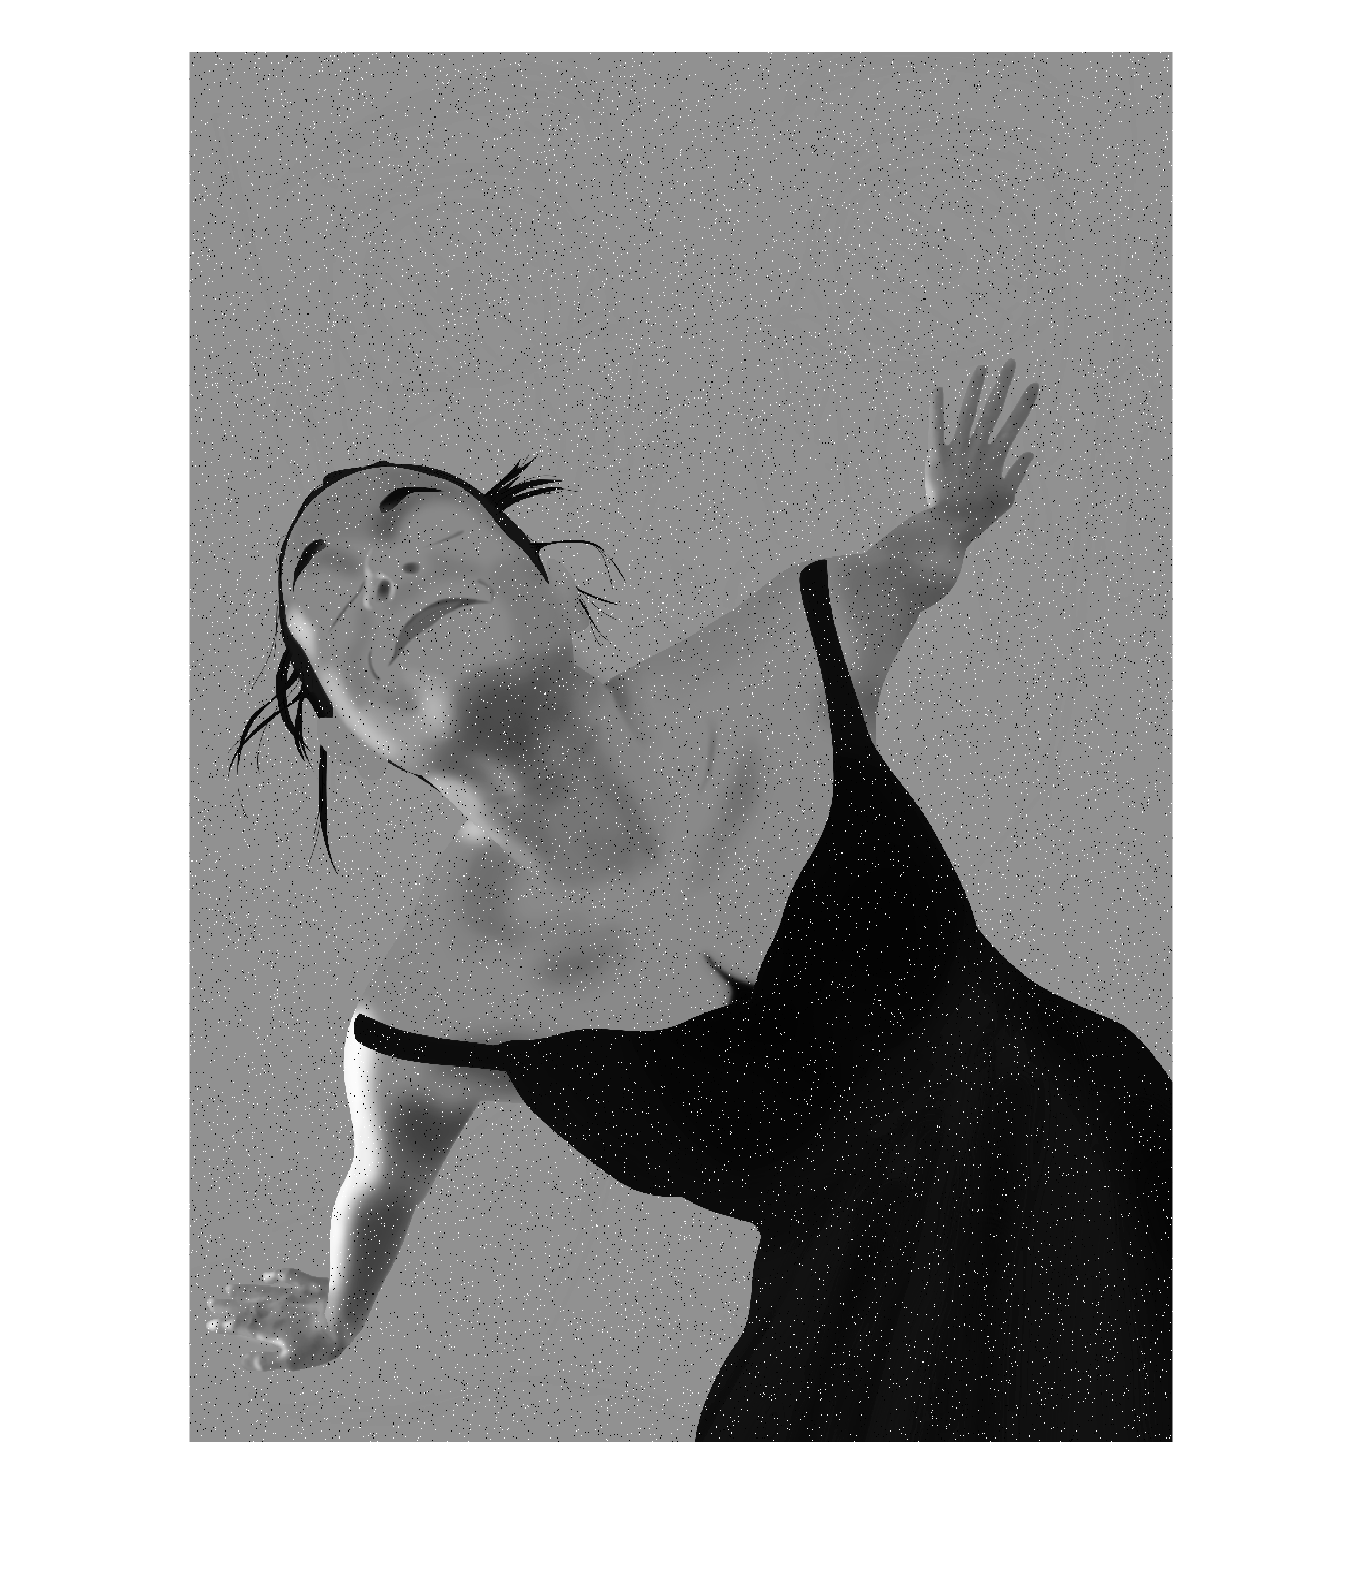
\includegraphics[scale=0.13,trim={6cm 0 4.5cm 0},clip]{Pictures/Esempi di utilizzo/Esempio 1/Amira_con_rumore.png}
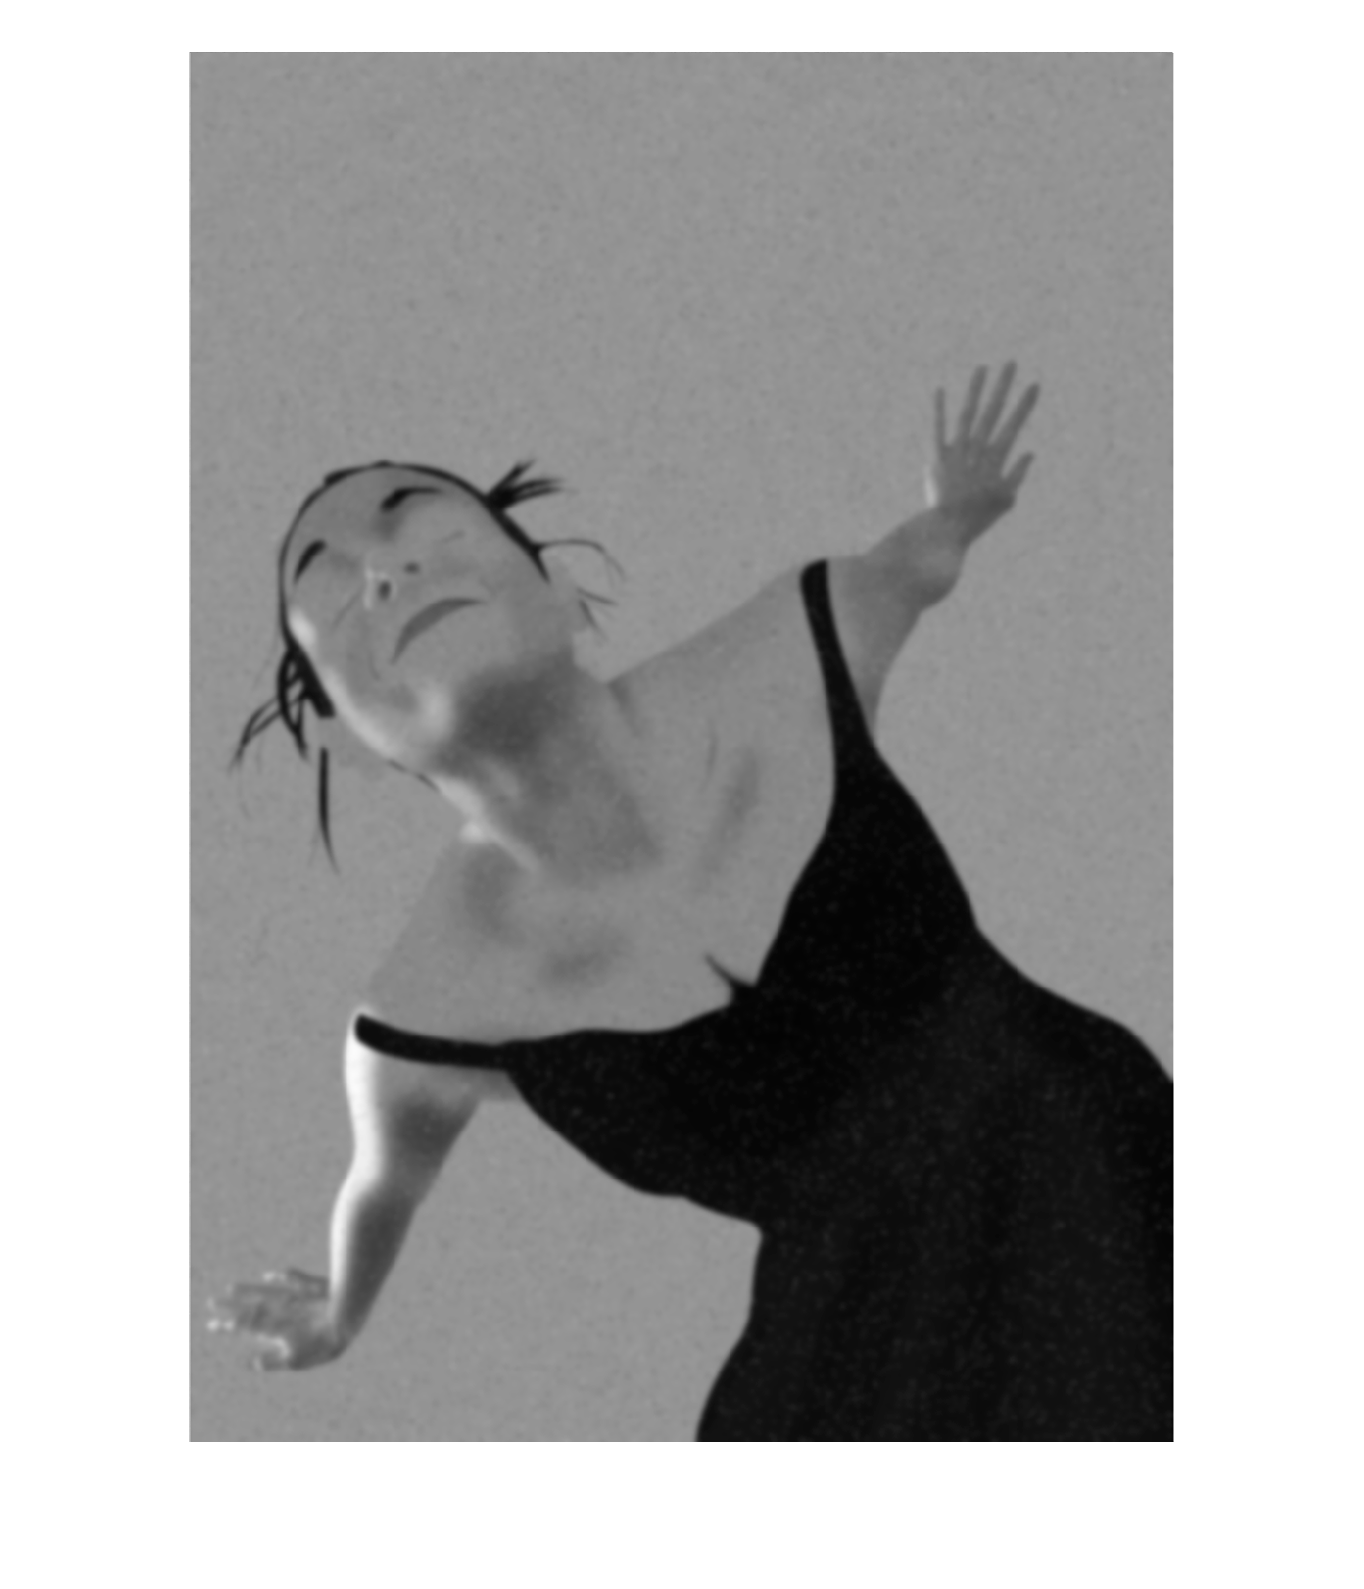
\includegraphics[scale=0.13,trim={6cm 0 6cm 0},clip]{Pictures/Esempi di utilizzo/Esempio 1/Amira_diffusa.png}
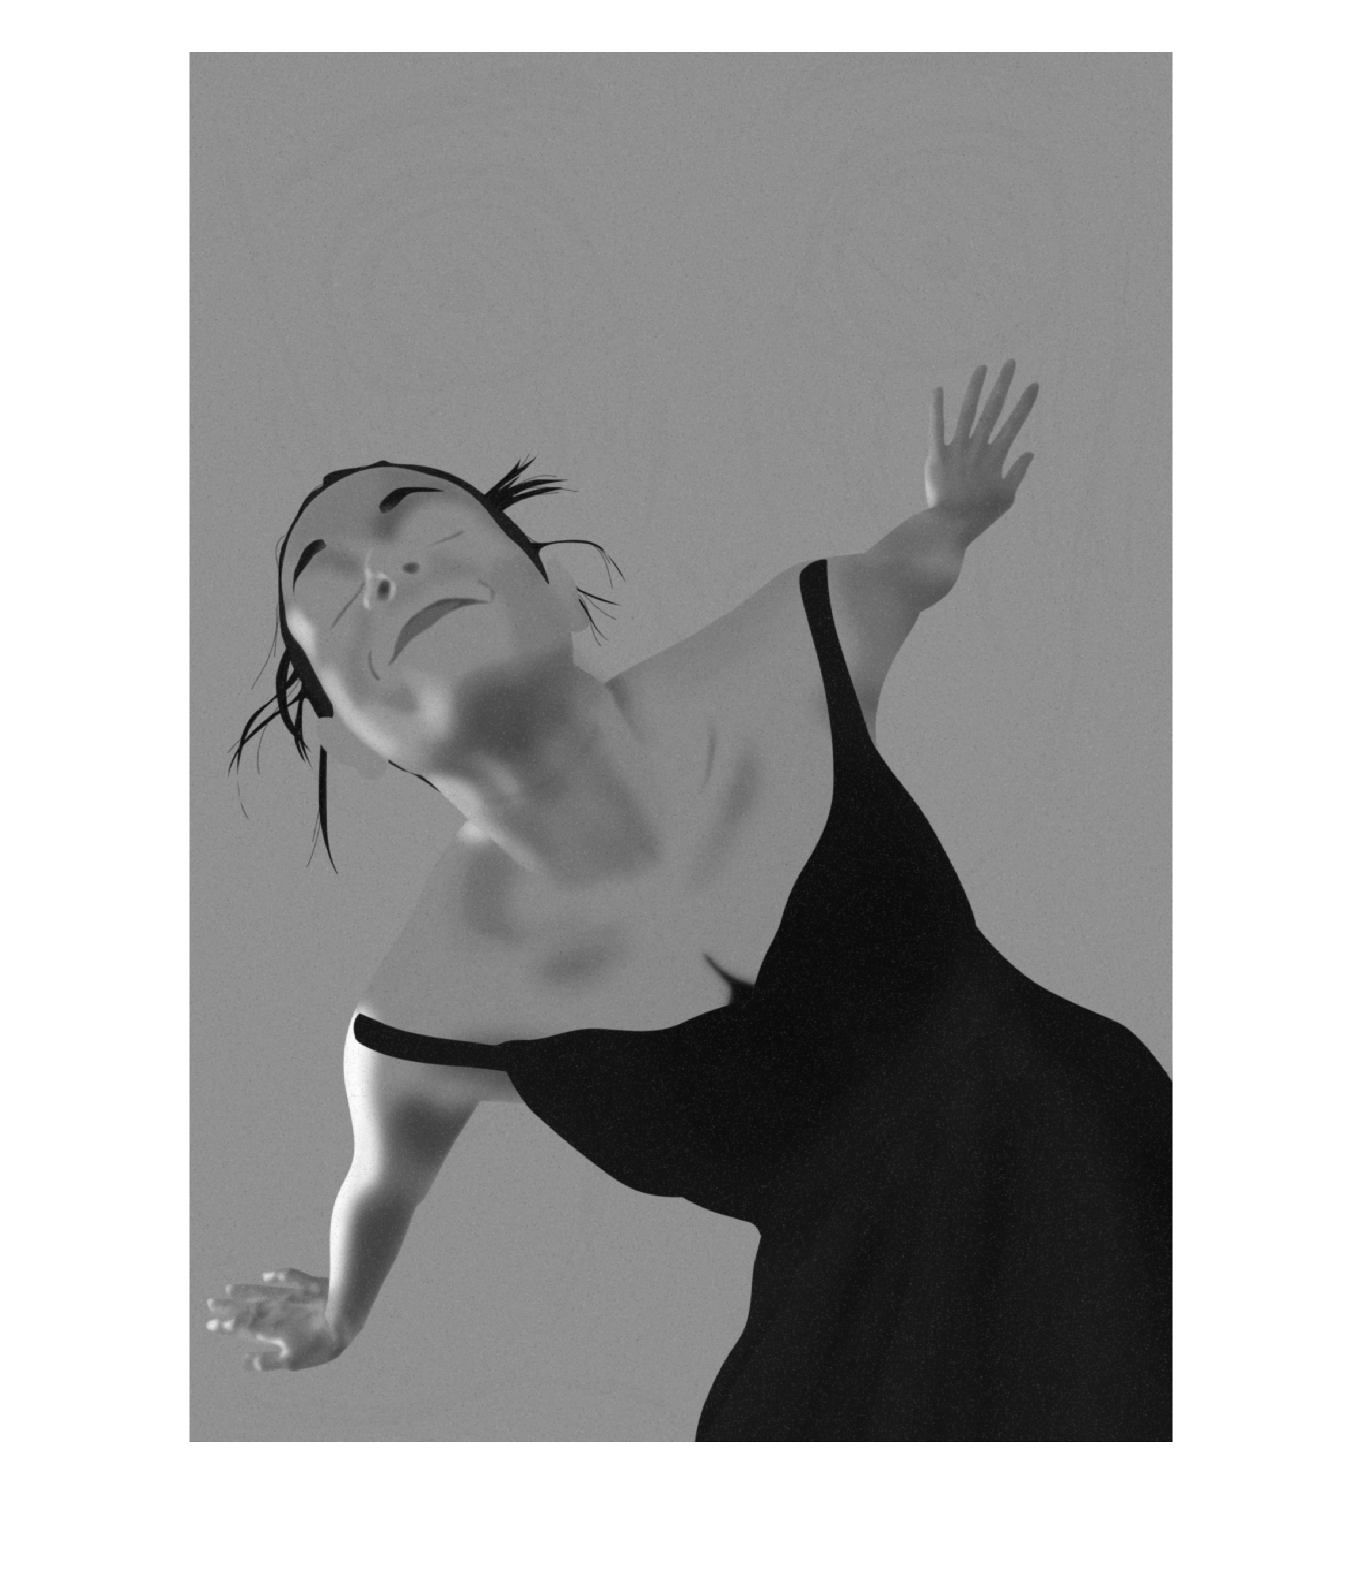
\includegraphics[scale=0.13,trim={4.5cm 0 6cm 0},clip]{Pictures/Esempi di utilizzo/Esempio 1/Amira_filtrata.png}
\caption{Da sinistra a destra: immagine con rumore, immagine filtrata con equazione del calore e immagine filtrata con metodo Perona-Malik.}\label{fig:figura}
\end{figure} 
Per brevità d'ora in avanti ci riferiremo a questi parametri come parametri standard.

\newpage
\subsection{Esempio 2 - Variazione del numero di iterazioni}
Andiamo adesso a vedere come il numero di iterazioni influisce sul risultato\\
filtriamo la stessa immagine confrontando i risultati dopo 10 iterazioni, dopo 20 iterazioni (valore standard) e dopo 100 iterazioni.
Parametri:
\begin{itemize}
    \item num\_iter=10, 20, 100
    \item delta\_t=0.1
    \item c=60
    \item sigma=1
\end{itemize}

\begin{figure}[htb] \centering
%\includegraphics[scale=0.13]{Pictures/Esempi di utilizzo/Amira_originale.png}
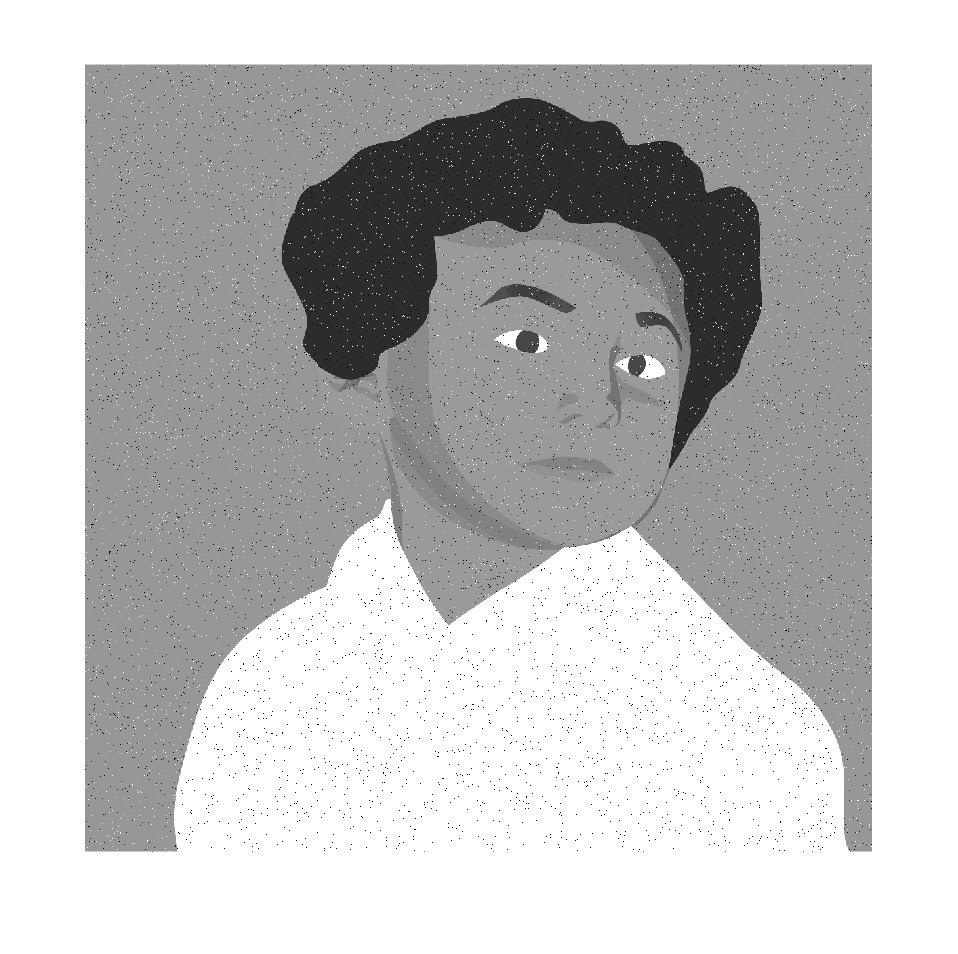
\includegraphics[scale=0.25]{Pictures/Esempi di utilizzo/Esempio 2/raffo_originale.png}
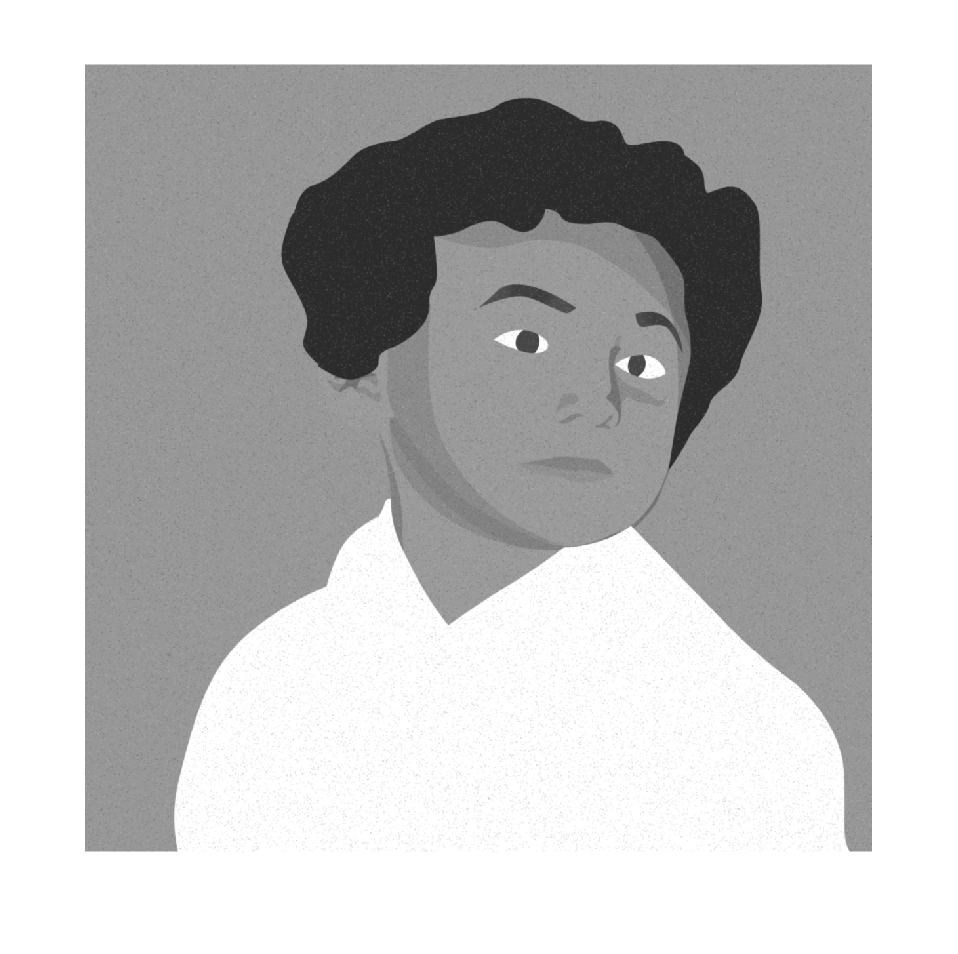
\includegraphics[scale=0.25]{Pictures/Esempi di utilizzo/Esempio 2/raffo_filtrata_n_iter10.png}
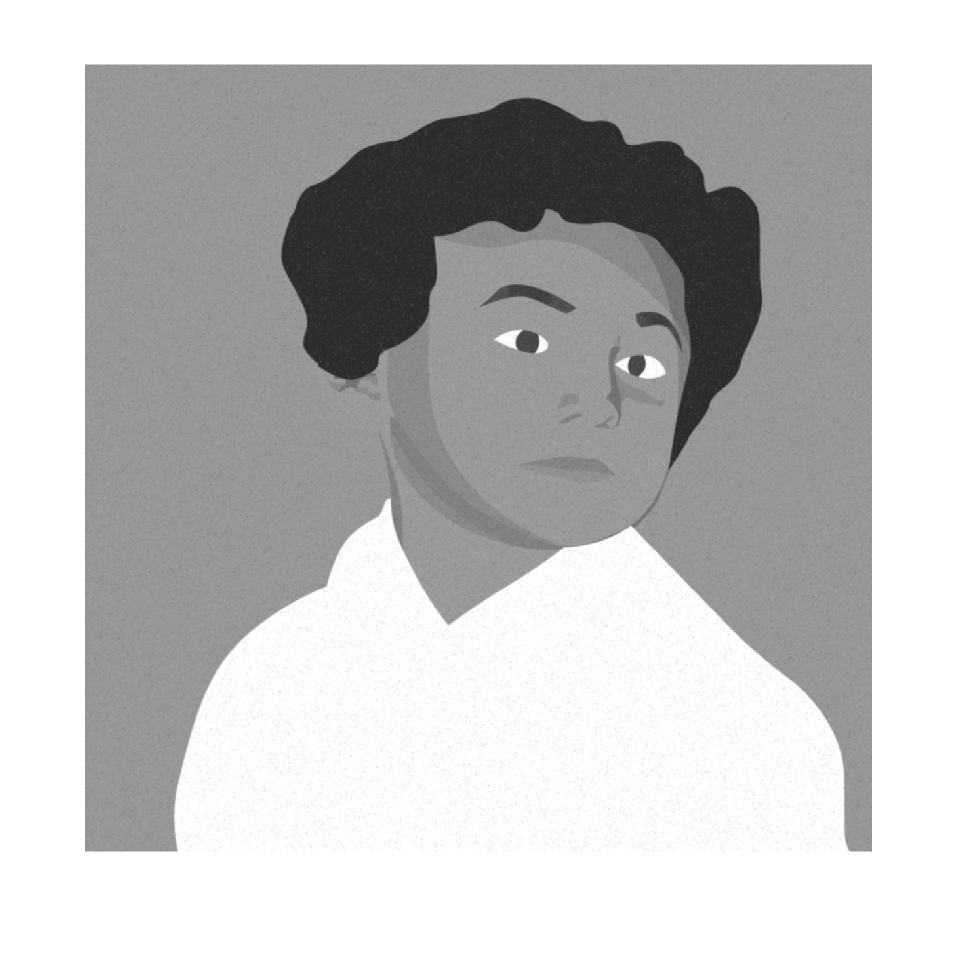
\includegraphics[scale=0.25]{Pictures/Esempi di utilizzo/Esempio 2/raffo_filtrata_n_iter20.png}
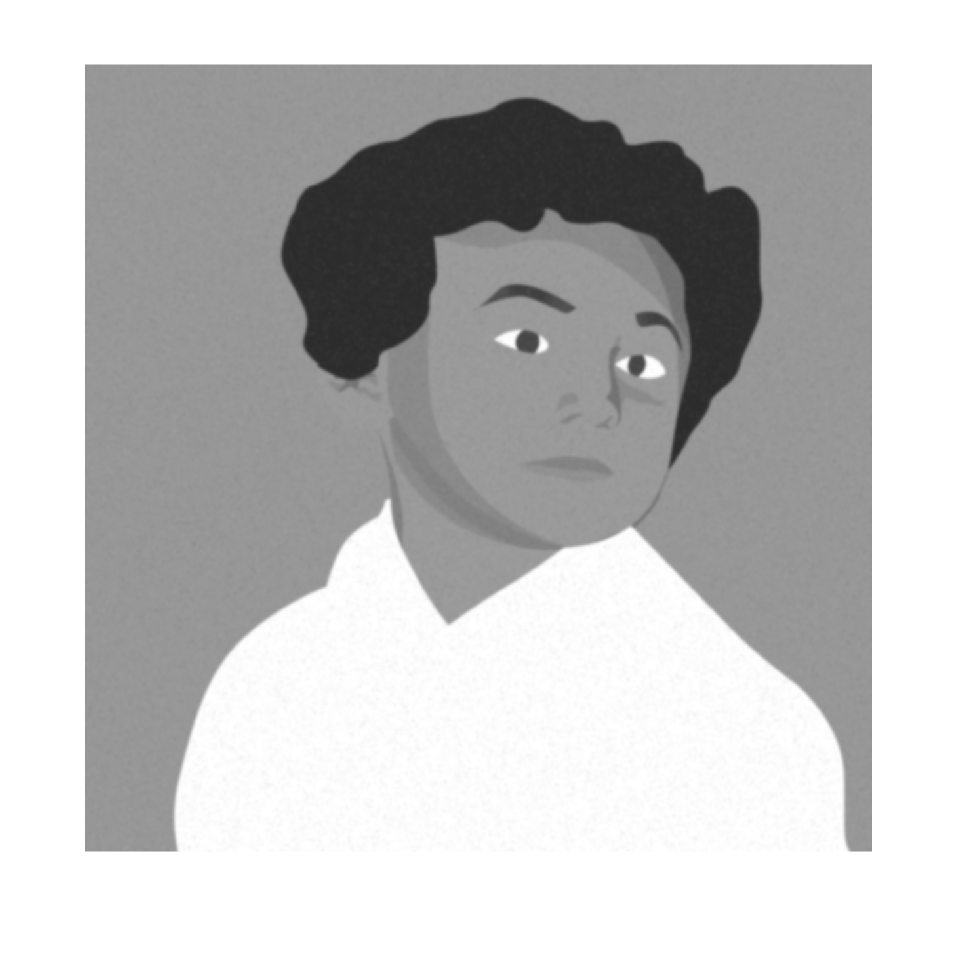
\includegraphics[scale=0.25]{Pictures/Esempi di utilizzo/Esempio 2/raffo_filtrata_n_iter100.png}
\caption{In ordine: immagine con rumore e immagine filtrata dopo 10 iterazioni, dopo 20 iterazioni e dopo 100 iterazioni.}\label{fig:figura}
\end{figure} 
Per poter meglio apprezzare le differenze vediamo delle sezioni d'immagine\\

\begin{figure}[htb] \centering
%\includegraphics[scale=0.13]{Pictures/Esempi di utilizzo/Amira_originale.png}

\includegraphics[scale=0.25]{Pictures/Esempi di utilizzo/Esempio 2/raffo_originale_dettaglio.png}

\includegraphics[scale=0.25]{Pictures/Esempi di utilizzo/Esempio 2/raffo_filtrata_n_iter10_dettaglio.png}

\includegraphics[scale=0.25]{Pictures/Esempi di utilizzo/Esempio 2/raffo_filtrata_n_iter20_dettaglio.png}

\includegraphics[scale=0.25]{Pictures/Esempi di utilizzo/Esempio 2/raffo_filtrata_n_iter100_dettaglio.png}
\caption{In ordine: immagine con rumore e immagine filtrata dopo 10 iterazioni, dopo 20 iterazioni e dopo 100 iterazioni.}\label{fig:figura}
\end{figure} 
Tramite queste immagini possiamo apprezzare come ad ogni ulteriore iterazione il rumore venga ridotto, rovinando tuttavia i bordi. \'E dunque bene valutare quando sia il caso di aumentare il numero di iterazioni e quando no. Se l'immagine in esame presenta dei bordi molto marcati, come ad esempio una scritta converrà preservarli il più possibile. Al contrario se l'immagine è caratterizzata per lo più da sfocature ci si può concedere di aumentare il numero di iterazioni.\\
\'E bene ricordare però che aumentare il numero di iterazioni porta un notevolmente aumento del costo computazionale e dunque del tempo di elaborazione.

\newpage
\subsection{Esempio 3 - Variazione della costante d'integrazione}
Passiamo ora alla costante d'integrazione e come cambiarla influisca con i risultati.\\
Parametri:
\begin{itemize}
    \item num\_iter=20
    \item delta\_t=0.01, 0.1, 0.2
    \item c=60
    \item sigma=1
\end{itemize}

\begin{figure}[htb] \centering
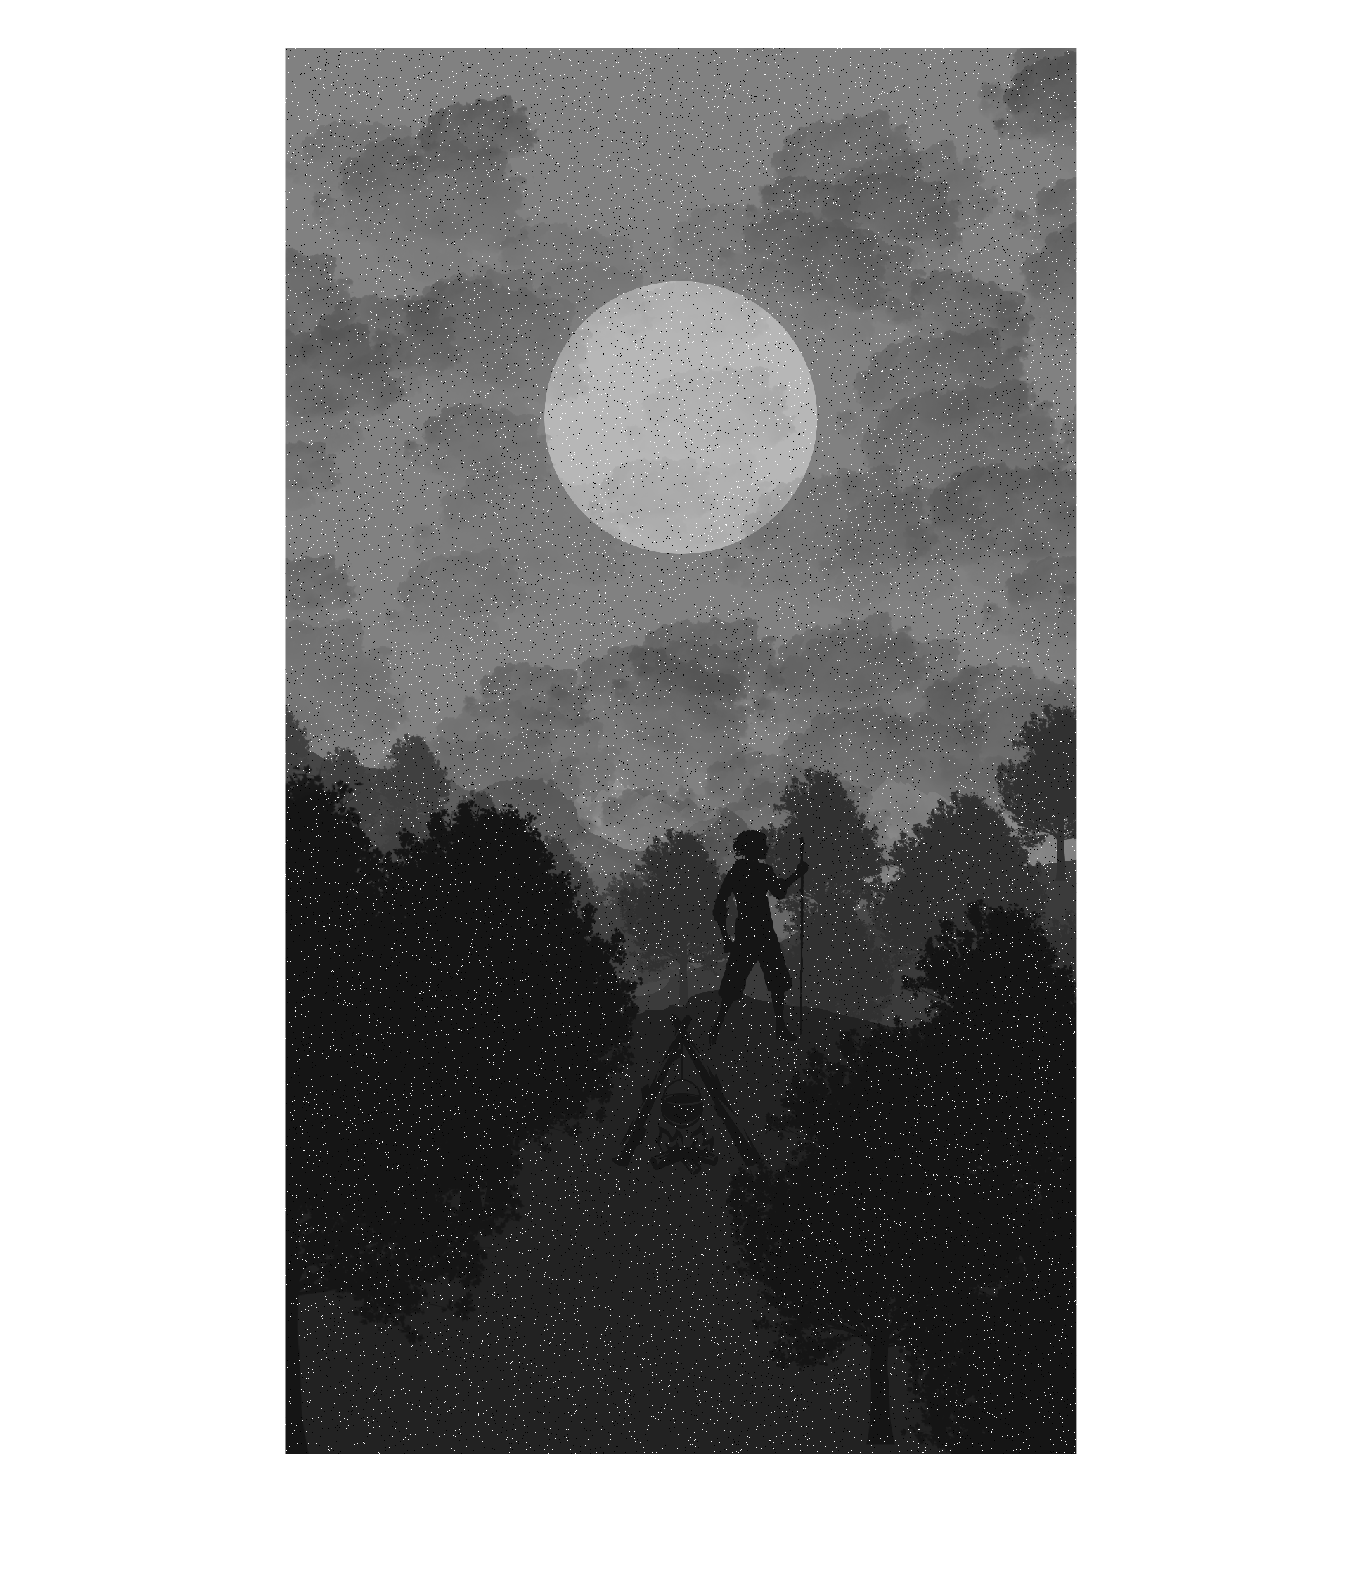
\includegraphics[scale=0.15]{Pictures/Esempi di utilizzo/Esempio 3/SfondoForesta_con_rumore.png}
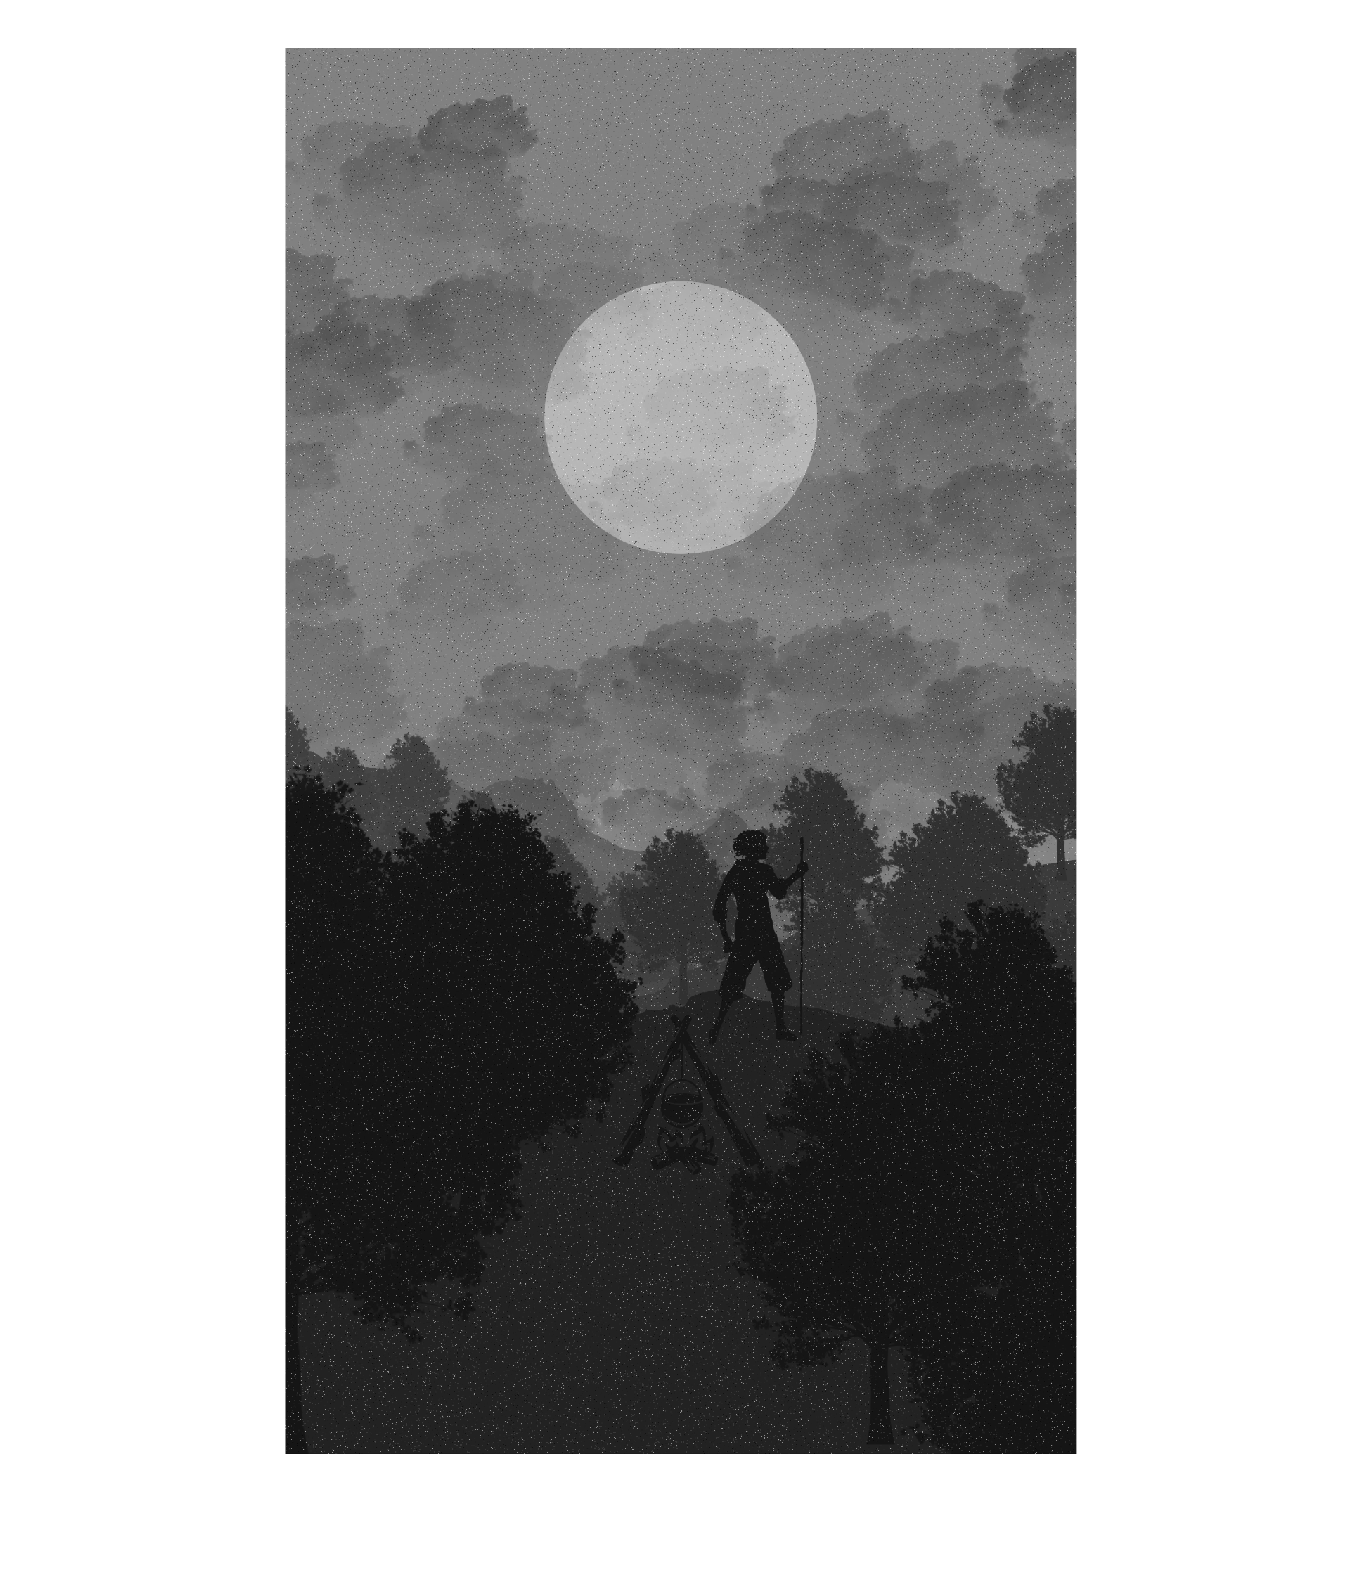
\includegraphics[scale=0.15]{Pictures/Esempi di utilizzo/Esempio 3/SfondoForesta_filtrata_deltat0_01.png}
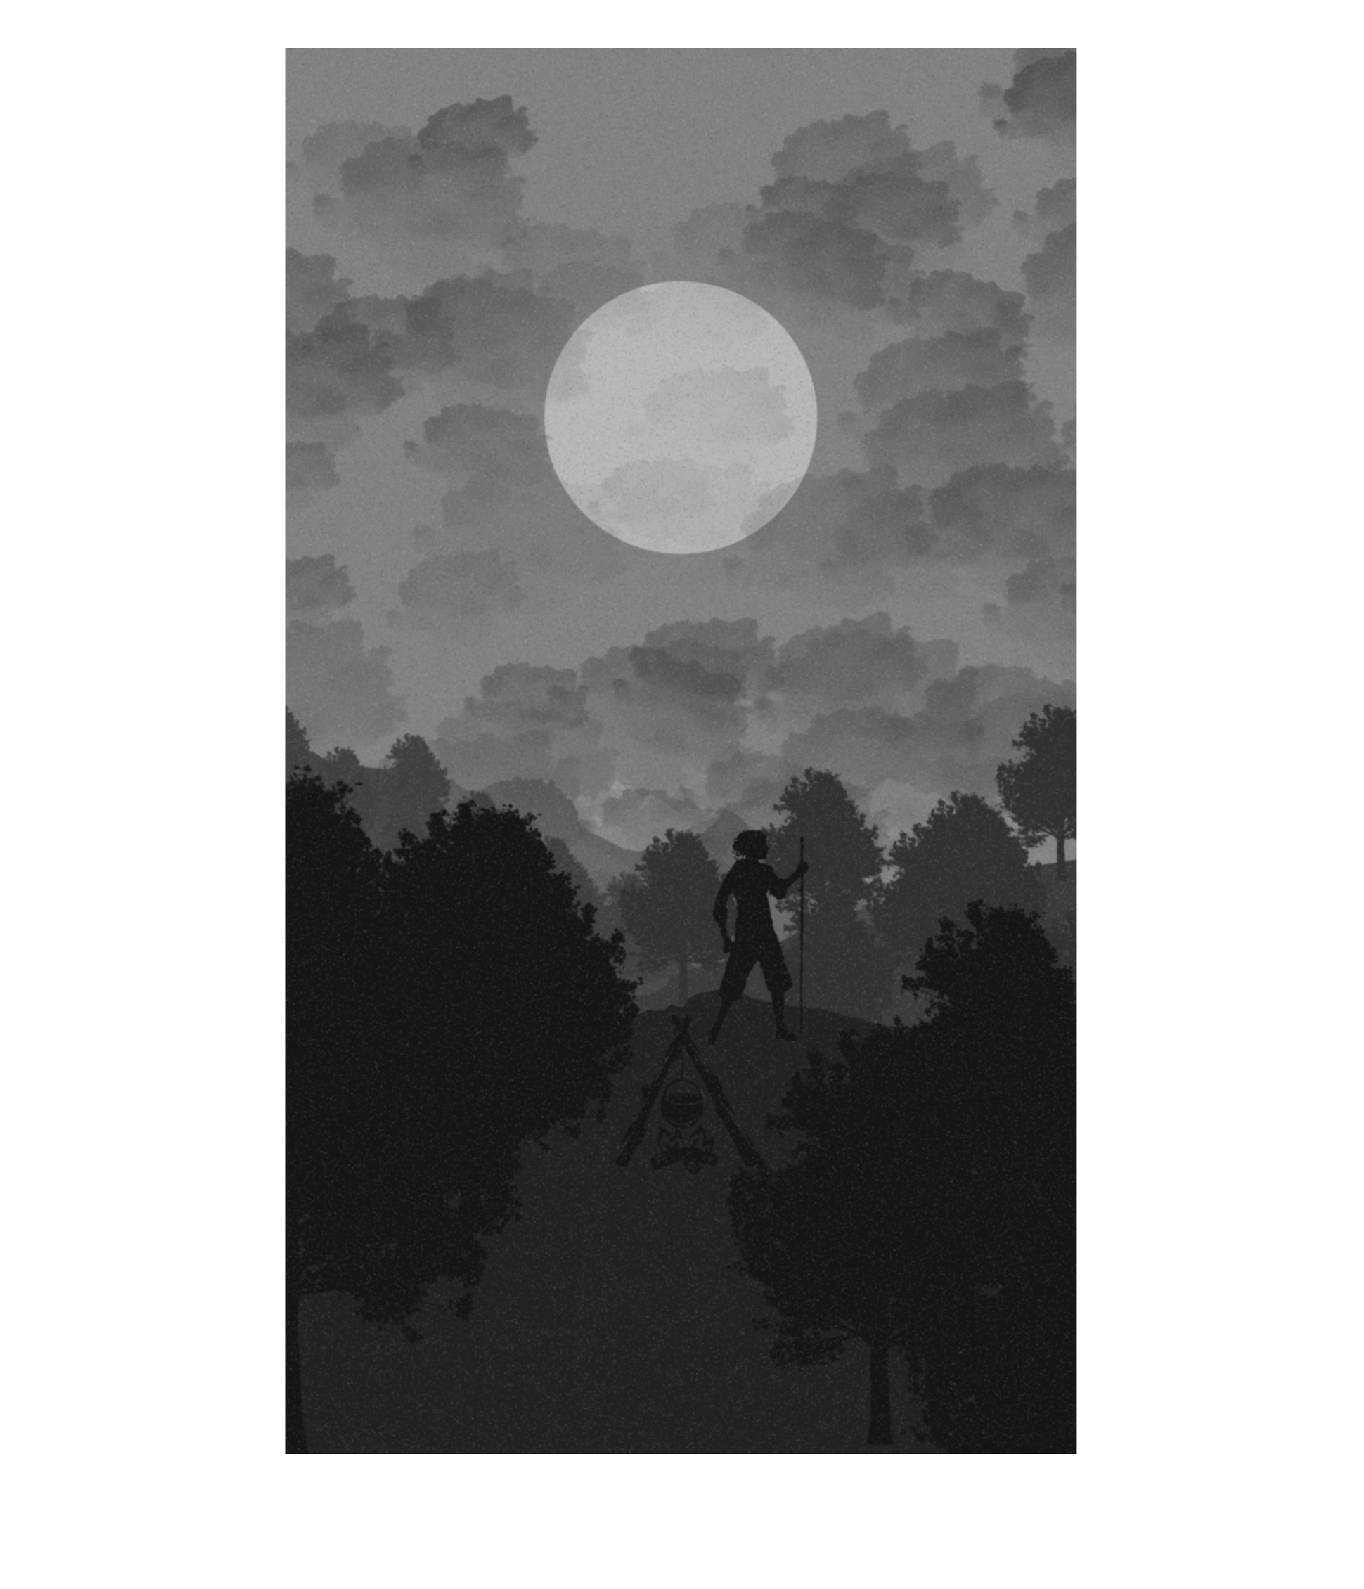
\includegraphics[scale=0.15]{Pictures/Esempi di utilizzo/Esempio 3/SfondoForesta_filtrata_deltat0_1.png}
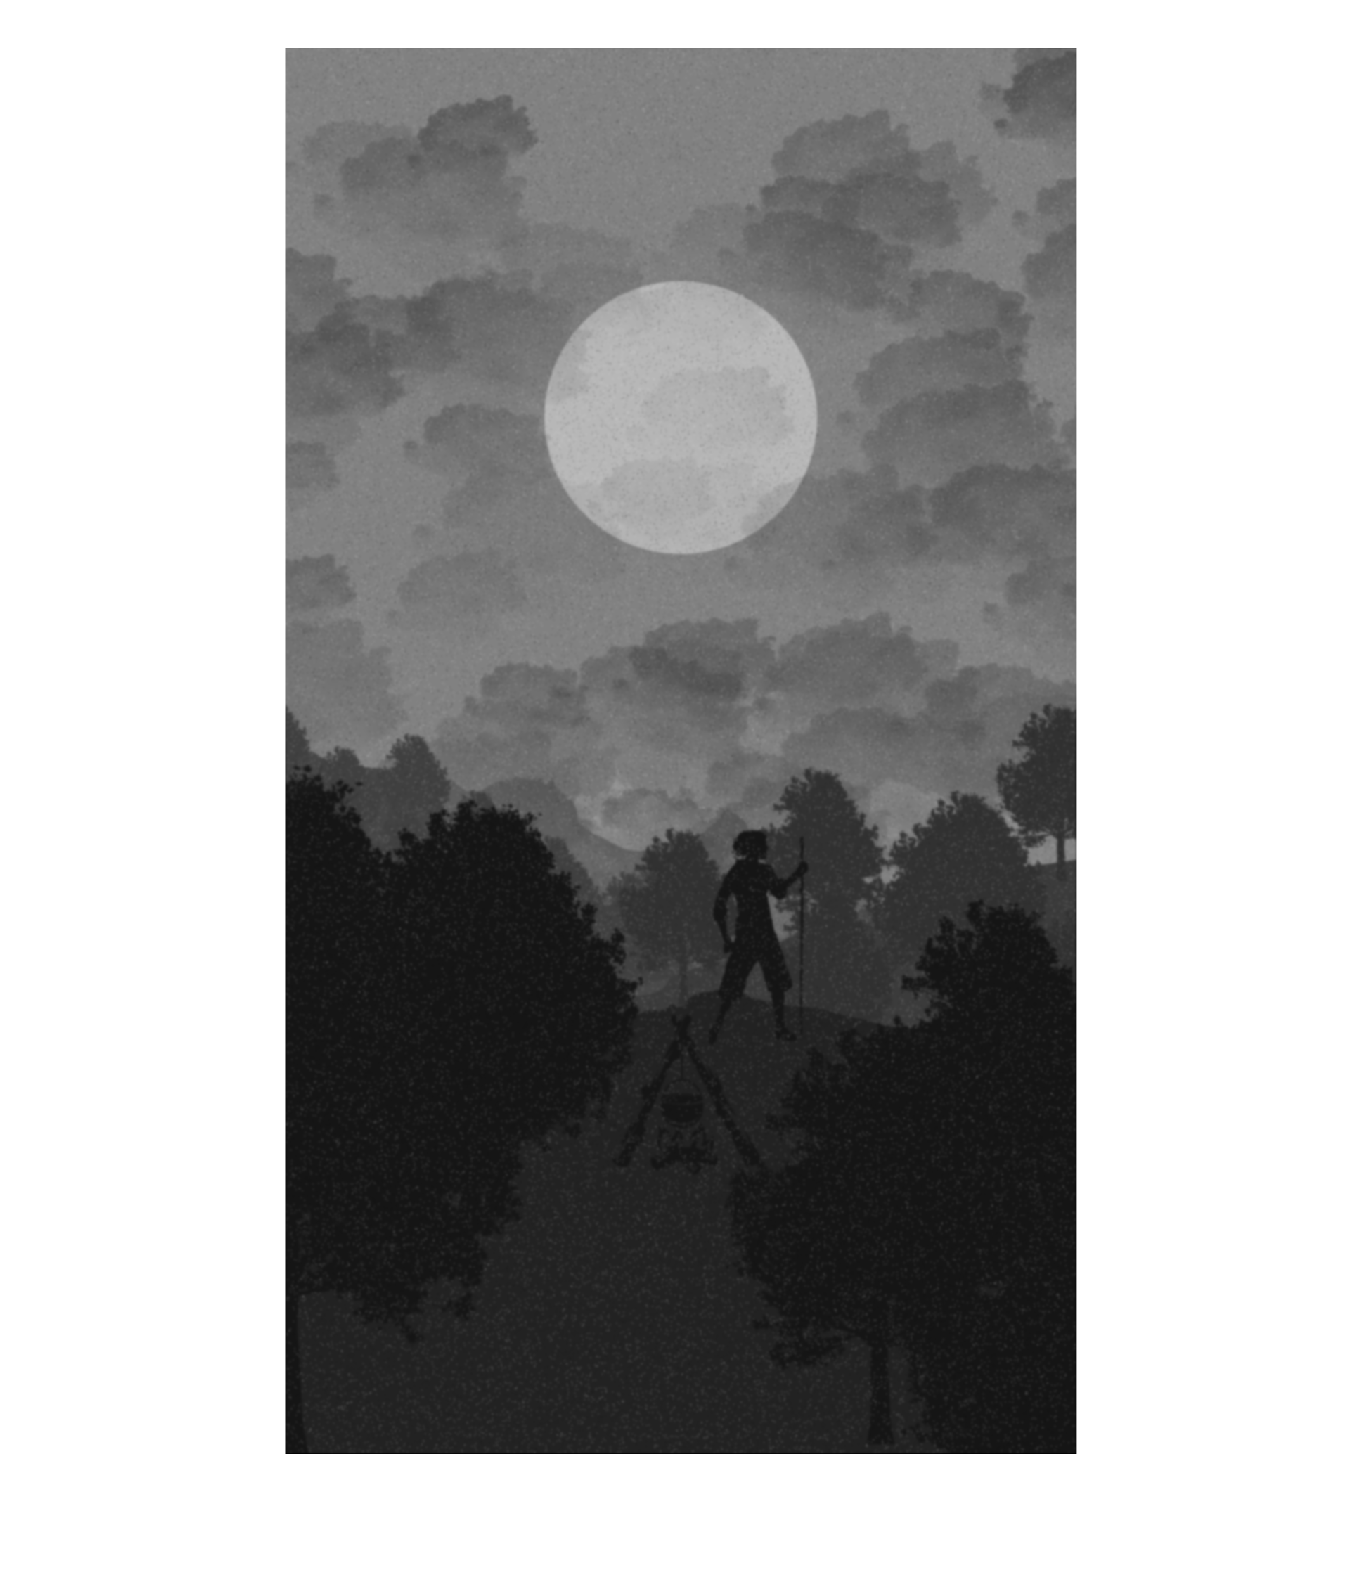
\includegraphics[scale=0.15]{Pictures/Esempi di utilizzo/Esempio 3/SfondoForesta_filtrata_deltat0_25.png}
\caption{In ordine: immagine con rumore, immagine filtrata con delta\_t=0.01, con delta\_t=0.1 e con delta\_t=0.25.}\label{fig:figura}
\end{figure} 
Da queste immagini è chiaramente visibile che per delta\_t prossimo allo zero (in questo caso 0.01) il problema del rumore non viene risolto, Ma solo attenuato. d'altro canto aumentandone il valore si perdono informazioni sui bordi molto più velocemente. Per poter meglio apprezzare questa differenza guardiamo delle sezioni delle ultime due immagini\\

\begin{figure}[htb] \centering
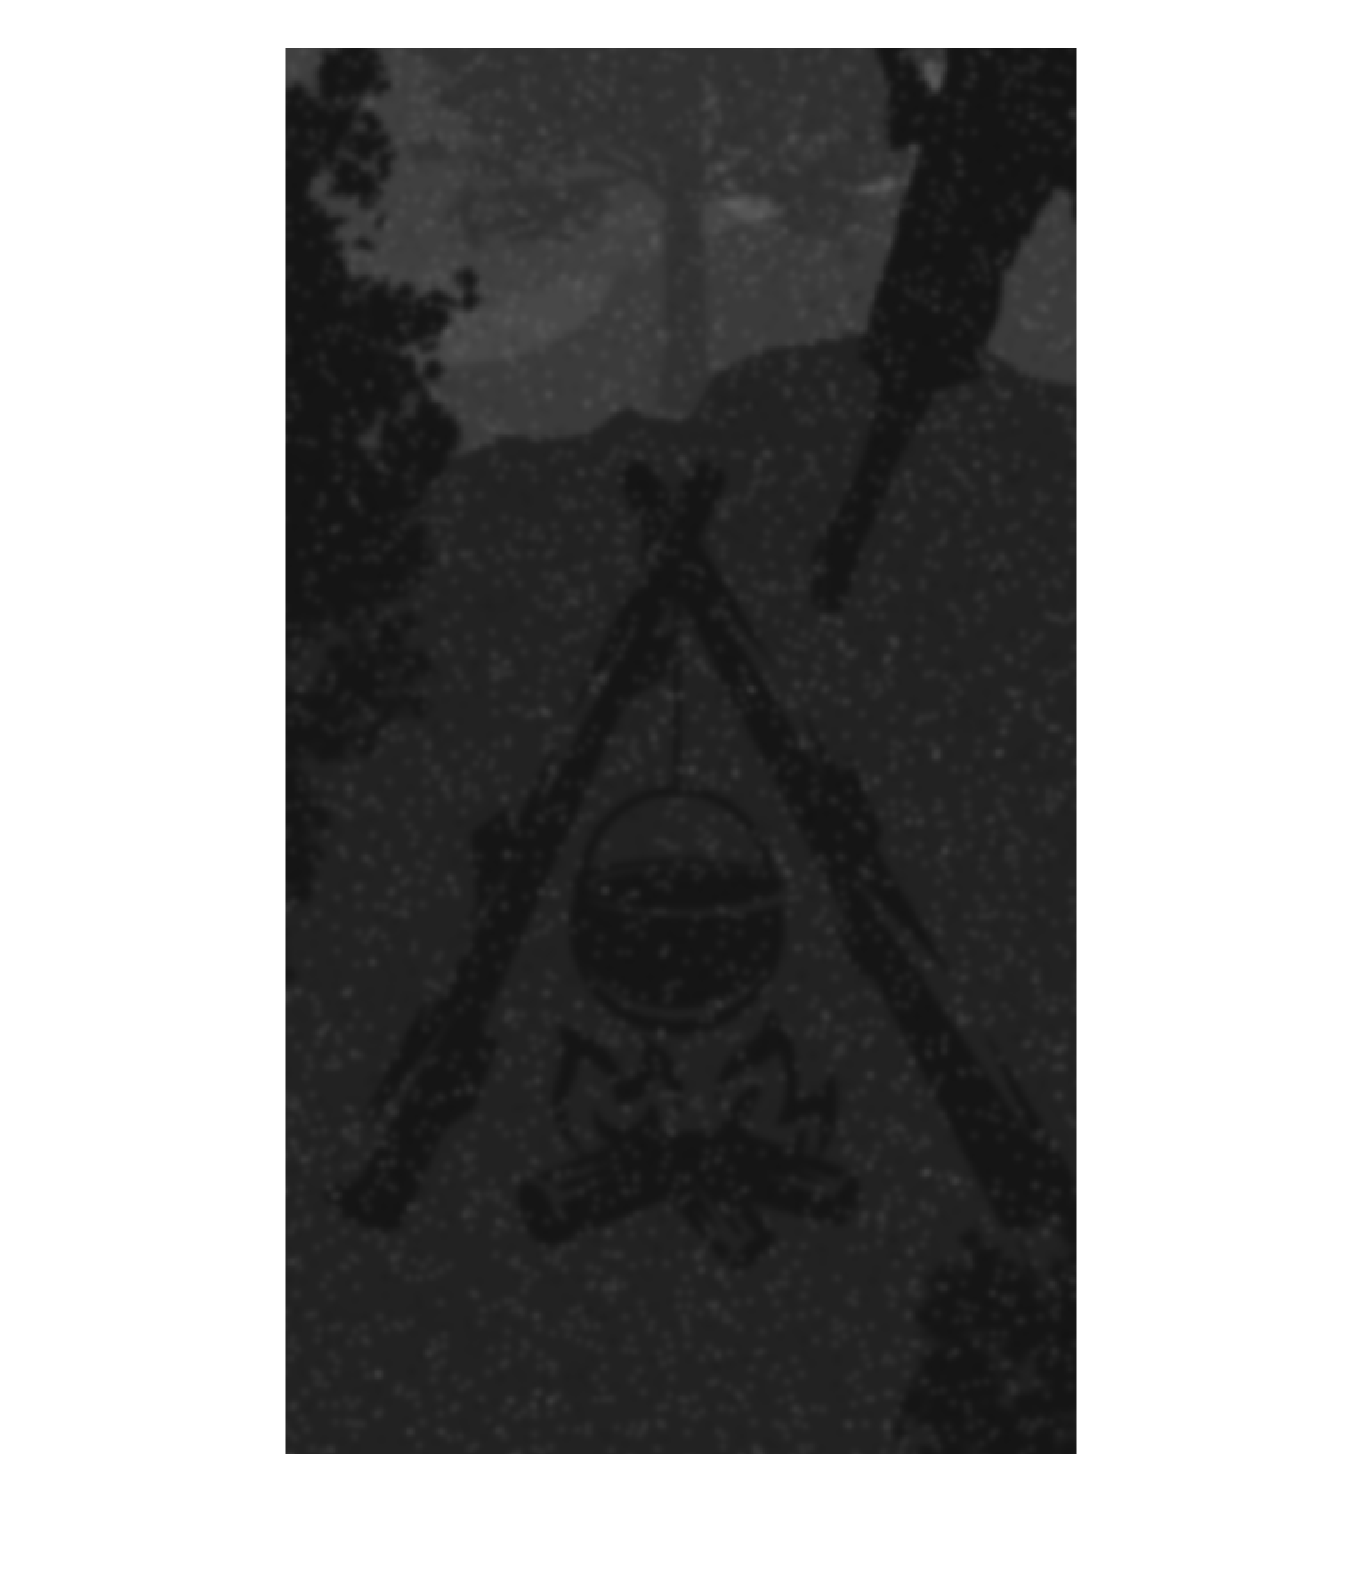
\includegraphics[scale=0.15]{Pictures/Esempi di utilizzo/Esempio 3/Dettaglio_SfondoForesta_filtrata_deltat0_1.png}
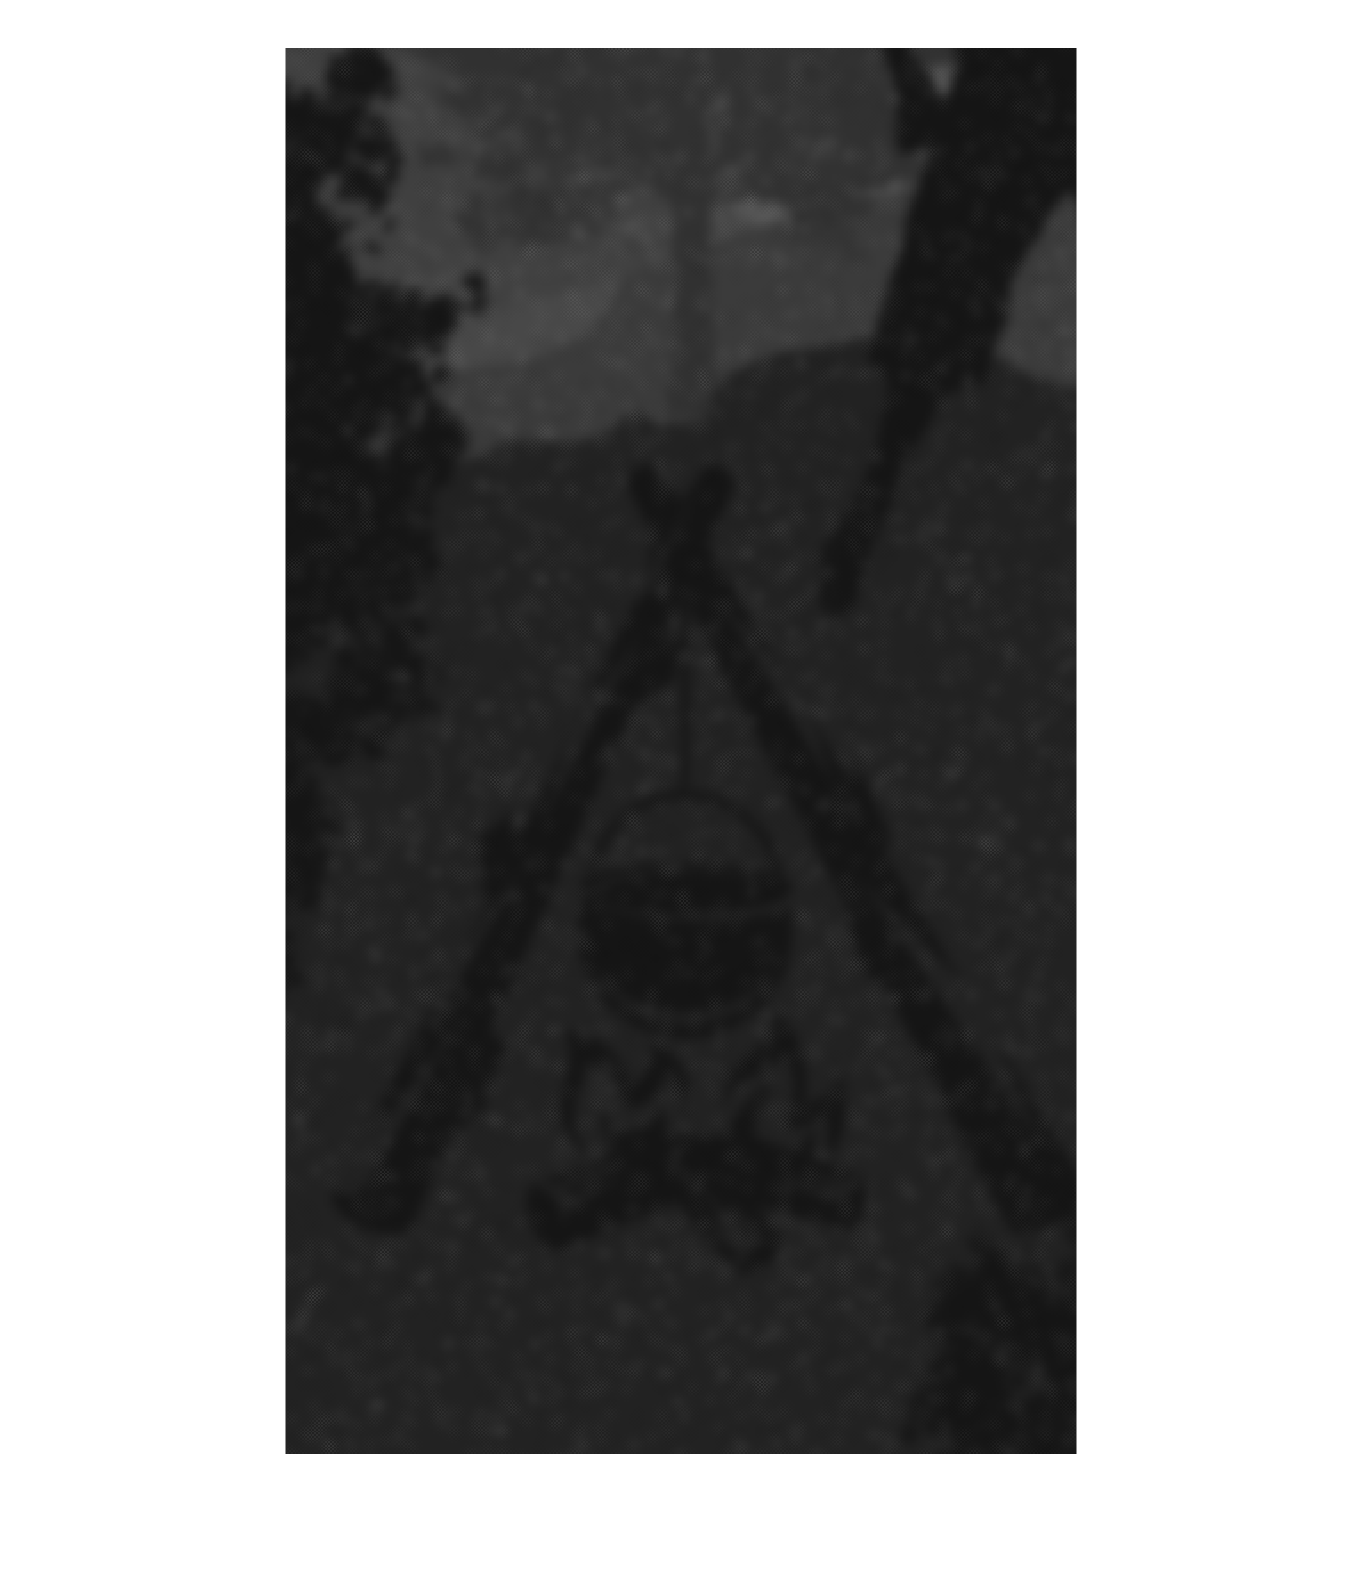
\includegraphics[scale=0.15]{Pictures/Esempi di utilizzo/Esempio 3/Dettaglio_SfondoForesta_filtrata_deltat0_25.png}
\caption{In ordine: immagine filtrata con delta\_t=0.1, e con delta\_t=0.25.}\label{fig:figura}
\end{figure} 

Vediamo quindi che aumentando questo parametro abbiamo un'immagine più sfuocata. Bisogna però fare attenzione poiché un valore anche solo di poco più alto può portare ad effetti distruttivi sull'immagine. Poniamo ad esempio delta\_t=0.3.

\begin{figure}[htb] \centering
\includegraphics[scale=0.15]{Pictures/Esempi di utilizzo/Esempio 3/SfondoForesta_filtrata_deltat0_3.png}
\caption{Immagine filtrata con delta\_t=0.3.}\label{fig:figura}
\end{figure}
Questa evidenza sperimentale conferma quanto visto nell'\textbf{Osservazione 2.2.1}. Per garantire la stabilità numerica occorre quindi utilizzare valori $delta\_t \in [0,\frac{1}{4}]$.

\newpage
\subsection{Esempio 4 - Variazione della costante di controllo}
Adesso vediamo la costante c di controllo, la quale influenza il coefficiente c che è ciò che caratterizza il metodo differenziandolo dalla sola applicazione dell'equazione del calore. Vediamo come questo parametro regola in che misura i bordi verranno preservati e come cambiarla influisca con i risultati.\\
Parametri:
\begin{itemize}
    \item num\_iter=20
    \item delta\_t=0.1
    \item c=6, 20, 60
    \item sigma=1
\end{itemize}

\begin{figure}[htb] \centering
\includegraphics[scale=0.15,trim={0 3cm 0 5cm},clip]{Pictures/Esempi di utilizzo/Esempio 4/party_originale.png}
\includegraphics[scale=0.15,trim={0 3cm 0 5cm},clip]{Pictures/Esempi di utilizzo/Esempio 4/party_filtrata_kappa6.png}
\includegraphics[scale=0.15,trim={0 5cm 0 3cm},clip]{Pictures/Esempi di utilizzo/Esempio 4/party_filtrata_kappa20.png}
\includegraphics[scale=0.15,trim={0 5cm 0 3cm},clip]{Pictures/Esempi di utilizzo/Esempio 4/party_filtrata_kappa60.png}
\caption{In ordine: immagine con rumore, immagine filtrata con c=6, con c=20 e con c=60.}\label{fig:figura}
\end{figure} 
Questi esempi ci permettono di apprezzare come al crescere di c abbiamo una maggior riduzione del rumore, mentre i bordi vengono preservati meno.\\
Analiticamente $c=c(|\frac{\nabla(u)}{k}|^2)\Longrightarrow$ al crescere i bordi vengono preservati meno.\\

\newpage
\subsubsection{Casi limite: c alto}
\begin{itemize}
    \item num\_iter=20
    \item delta\_t=0.1
    \item c=60000
    \item sigma=1
\end{itemize}

\begin{figure}[htb] \centering
\includegraphics[scale=0.15,trim={0 3cm 0 5cm},clip]{Pictures/Esempi di utilizzo/Esempio 4/party_caso_limite_kappaalto.png}
\includegraphics[scale=0.15,trim={0 3cm 0 5cm},clip]{Pictures/Esempi di utilizzo/Esempio 4/party_caso_limite_eq_calore.png}
\caption{In ordine: immagine filtrata con c=60000 e immagine filtrata con equazione del calore.}\label{fig:figura}
\end{figure} 
Analogamente, con un valore molto alto possiamo vedere che l'immagine sembra solamente diffusa, e infatti $c=c(|\frac{\nabla(u)}{k}|^2)\Longrightarrow\lim_{k\to\infty}c(|\frac{\nabla(u)}{k}|^2)=1$.\\
Ma allora $\frac{\partial u}{\partial t}(t,x)=div(c\nabla(u))=div(\nabla(u))=\Delta(u)$ ritrovando quindi l'equazione del calore, numericamente infatti troviamo:
\texttt{min(min([cN,cS,cW,cE]))=0.999996871393924} e \texttt{max(max([cN,cS,cW,cE]))=1}
riconosciamo quindi un appiattimento di c ad 1.

\newpage
\subsubsection{Casi limite: c basso}
Parametri:
\begin{itemize}
    \item num\_iter=20
    \item delta\_t=0.1
    \item c=0.001
    \item sigma=1
\end{itemize}

\begin{figure}[htb] \centering
\includegraphics[scale=0.15,trim={0 3cm 0 5cm},clip]{Pictures/Esempi di utilizzo/Esempio 4/party_caso_limite_originale.png}
\includegraphics[scale=0.15,trim={0 3cm 0 5cm},clip]{Pictures/Esempi di utilizzo/Esempio 4/party_caso_limite_kappabasso.png}
\caption{In ordine: immagine con rumore e immagine filtrata con c=0.001.}\label{fig:figura}
\end{figure} 
Possiamo facilmente notare come con un valore molto basso di c l'immagine sembra non subire variazioni, effettivamente
$c=c(|\frac{\nabla(u)}{k}|^2)\Longrightarrow\lim_{k\to0}c(|\frac{\nabla(u)}{k}|^2)=0$.\\
Ma allora $\frac{\partial u}{\partial t}(t,x)=div(c\nabla(u))=div(0*\nabla(u))=0$, ma $\frac{\partial u}{\partial t}(t,x)=0 \Leftrightarrow u=cost$ cioè non c'è variazione.\\
In questo caso non riportiamo i dati sul massimo e sul minimo di c perché anche se ci aspettiamo un appiattimento sullo 0 ci sarà sicuramente qualche punto in cui non c'è variazione di colore la derivata sarà quindi nulla e per quanto piccolo possiamo scegliere k il rapporto farà comunque 0 e quindi c sarà 1. Questo non ci preoccupa siccome il metodo sfocherà una porzione d'immagine di colore costante per cui anche in questi punti non avremo nessuna variazione

\newpage
\subsection{Esempio 5  - Variazione della costante di diffusione}
Adesso vediamo la costante Sigma, la quale regola l'applicazione dell'equazione del calore che influenza il coefficiente c. Vediamo quindi anche in questo caso come questo parametro regola in che misura i bordi verranno preservati e come cambiarla influisca con i risultati.\\
Parametri:
\begin{itemize}
    \item num\_iter=20
    \item delta\_t=0.1
    \item c=60
    \item sigma=0.5, 1, 2
\end{itemize}

\begin{figure}[htb] \centering
\includegraphics[scale=0.15,trim={0cm 3cm 3cm 0cm},clip]{Pictures/Esempi di utilizzo/Esempio 5/ami_originale_resize.png}
\includegraphics[scale=0.15,trim={3cm 3cm 0cm 0cm},clip]{Pictures/Esempi di utilizzo/Esempio 5/ami_filtrata_sigma0_5_kappa60_resize.png}
\includegraphics[scale=0.15,trim={0cm 0cm 3cm 0cm},clip]{Pictures/Esempi di utilizzo/Esempio 5/ami_filtrata_sigma1_kappa60_resize.png}
\includegraphics[scale=0.15,trim={3cm 0cm 0cm 0cm},clip]{Pictures/Esempi di utilizzo/Esempio 5/ami_filtrata_sigma2_kappa60_resize.png}
\caption{In ordine: immagine con rumore, immagine filtrata con sigma=0.5, con sigma=1 e con sigma=2.}\label{fig:figura}
\end{figure} 
Questi esempi però non ci permettono di apprezzare una gran differenza, infatti sigma influenza il gradiente, questo va però diviso per c che in questo caso è 60 appiattendo i valori del gradiente.\\
Infatti, $\frac{\nabla(u)_1}{k}-\frac{\nabla(u)_2}{k}=\frac{\nabla(u)_1-\nabla(u)_2}{k}$ cioè anche la differenza tra i due gradienti sarà 60 volte minore e quindi poco visibile.\\
Per rendere più evidenti queste differenze possiamo allora abbassare il valore di k.\\
Parametri:
\begin{itemize}
    \item num\_iter=20
    \item delta\_t=0.1
    \item c=0.5
    \item sigma=0.5, 1, 2
\end{itemize}

\begin{figure}[htb] \centering
\includegraphics[scale=0.15,trim={0cm 3cm 3cm 0cm},clip]{Pictures/Esempi di utilizzo/Esempio 5/ami_originale_resize.png}
\includegraphics[scale=0.15,trim={3cm 3cm 0cm 0cm},clip]{Pictures/Esempi di utilizzo/Esempio 5/ami_filtrata_sigma0_5_resize.png}
\includegraphics[scale=0.15,trim={0cm 0cm 3cm 0cm},clip]{Pictures/Esempi di utilizzo/Esempio 5/ami_filtrata_sigma1_resize.png}
\includegraphics[scale=0.15,trim={3cm 0cm 0cm 0cm},clip]{Pictures/Esempi di utilizzo/Esempio 5/ami_filtrata_sigma2_resize.png}
\caption{In ordine: immagine con rumore, immagine filtrata con sigma=0.5, con sigma=1 e con sigma=2.}\label{fig:figura}
\end{figure} 
Anche in questo caso, come visto nell'esempio 3, bisogna fare attenzione a non impostare valori troppo alti. Nell'esempio 3 ce ne siamo preoccupati perchè il metodo prevede il calcolo \texttt{diff\_im = diff\_im + delta\_t*(cN.*nablaN + cS.*nablaS + cW.*nablaW + cE.*nablaE)} e si era detto che per garantire la stabilità numerica utilizziamo $delta\_t \in [0,\frac{1}{4}]$.
Ricordiamo adesso che per operare il filtraggio richiamiamo l'equazione del calore, che invece prevede il calcolo \texttt{u= u + sigma*dt*(u\_{xx}+u\_{yy})}, per cui per assicurare la stabilità numerica imponiamo anche $delta\_t*sigma \in[0,\frac{1}{4}]$, in accordo con quanto visto nella \textbf{Proposizione 2.1.1}. Vediamo ad esempio quali risultati otteniamo ponendo sigma=2, che abbiamo visto dare un buon risultato, e delta\_t=0.2.\\
Parametri:
\begin{itemize}
    \item num\_iter=20
    \item delta\_t=0.2
    \item c=0.5
    \item sigma=2
\end{itemize}

\begin{figure}[htb] \centering
\includegraphics[scale=0.15,trim={3cm 0cm 3cm 0cm},clip]{Pictures/Esempi di utilizzo/Esempio 5/ami_originale_resize.png}
\includegraphics[scale=0.15,trim={3cm 0cm 3cm 0cm},clip]{Pictures/Esempi di utilizzo/Esempio 5/ami_calore_sigma2_deltat0_2_resize.png}
\includegraphics[scale=0.15,trim={3cm 0cm 3cm 0cm},clip]{Pictures/Esempi di utilizzo/Esempio 5/ami_filtrata_sigma2_deltat0_2_resize.png}
\caption{In ordine: immagine originale, immagine filtrata con equazione del calore e immagine filtrata con sigma=2.}\label{fig:figura}
\end{figure} 
Otteniamo quindi un'immagine quasi non filtrata, numericamente infatti troviamo:
\texttt{min(min([cN,cS,cW,cE]))=0} e \texttt{max(max([cN,cS,cW,cE]))=4.3775e-106}
riconosciamo quindi un appiattimento di c sullo 0.


\bibliography{references}



\end{document}

\







